\documentclass[12pt,a4paper]{memoir}   

% No fraccionar palabras
\sloppy
% Margenes del documento

%  Horizontal 
\setlength{\hoffset}{0pt}                  % [ 1 ] 
\setlength{\oddsidemargin}{1.46cm}       % [ 3 ]
\setlength{\evensidemargin}{-0.54cm}    % [ 3 ] 
\setlength{\textwidth}{425pt}            % [ 8 ]
\setlength{\marginparsep}{7pt}        % [ 9 ]
\setlength{\marginparwidth}{106pt}  % [10]

% Vertical 
\setlength{\voffset}{-40pt}              %  [ 2 ]
\setlength{\topmargin}{22pt}                % [ 4 ]
\setlength{\headheight}{25pt} % [ 5 ]
\setlength{\headsep}{35pt} % [ 6 ]
\setlength{\textheight}{600pt} %[ 7 ]
\renewcommand{\footskip}{75pt} % [11]

\parindent=0pt

% Formato de los capitulos
\usepackage{fourier} 
\usepackage[scaled=.92]{helvet}%. Sans serif - Helvetica
\usepackage{color,calc}
\newsavebox{\ChpNumBox}
\makeatletter
\newcommand*{\thickhrulefill}{%
\leavevmode\leaders\hrule height 1\p@ \hfill \kern \z@}
\newcommand*\BuildChpNum[2]{%
\begin{tabular}[t]{@{}c@{}}
\makebox[0pt][c]{#1\strut} \\[.5ex]
\colorbox{gray75}{%
\rule[-5em]{0pt}{0pt}%
\rule{1ex}{0pt}\color{white}#2\strut
\rule{1ex}{0pt}}%
\end{tabular}}
\makechapterstyle{BlueBox}{%
\renewcommand{\chapnamefont}{\large\scshape}
\renewcommand{\chapnumfont}{\Huge\bfseries}
\renewcommand{\chaptitlefont}{\raggedright\Huge\bfseries}
\setlength{\beforechapskip}{20pt}
\setlength{\midchapskip}{26pt}
\setlength{\afterchapskip}{40pt}
\renewcommand{\printchaptername}{}
\renewcommand{\chapternamenum}{}
\renewcommand{\printchapternum}{%
\sbox{\ChpNumBox}{%
\BuildChpNum{\chapnamefont\@chapapp}%
{\chapnumfont\thechapter}}}
\renewcommand{\printchapternonum}{%
\sbox{\ChpNumBox}{%
\BuildChpNum{\chapnamefont\vphantom{\@chapapp}}%
{\chapnumfont\hphantom{\thechapter}}}}
\renewcommand{\afterchapternum}{}
\renewcommand{\printchaptertitle}[1]{%
\usebox{\ChpNumBox}\hfill
\parbox[t]{\hsize-\wd\ChpNumBox-1em}{%
\vspace{\midchapskip}%
\thickhrulefill\par
\chaptitlefont ##1\par}}%
}
\chapterstyle{BlueBox}
% BABLE - Idioma
\usepackage[spanish]{babel}
\usepackage[utf8]{inputenc}

% FANCYHDR - Para incluir cabeceras
\let\footruleskip\undefined
\usepackage{fancyhdr}
\pagestyle{fancy}

\renewcommand{\chaptermark}[1]{\markboth{\textbf{\thechapter. #1}}{}} % Formato para el capítulo: N. Nombre
\renewcommand{\sectionmark}[1]{\markright{\textbf{\thesection. #1}}} % Formato para la sección: N.M. Nombre


\renewcommand{\headrulewidth}{0.6pt} % Ancho de la línea horizontal bajo el encabezado
\renewcommand{\footrulewidth}{0.6pt} % Ancho de la línea horizontal sobre el pie (que en este ejemplo está vacío)

\renewcommand{\footnoterule}{\vspace*{15pt}\dotfill\hfill\vspace*{10pt}}

\fancyhf{}
\fancyhead[LE]{ 
\includegraphics[height=0.5in,width=0.5in]{imagenes/EscudoFacultad.jpg} \textbf{Capítulo} \leftmark} % En las páginas impares, parte izquierda del encabezado, aparecerá el nombre de capítulo
\fancyhead[RO]{\vspace*{0.36in}\rightmark} % En las páginas pares, parte derecha del encabezado, aparecerá el nombre de sección
%\fancyhead[RO,LE]{\thepage} % Números de página en las esquinas de los encabezados
\fancyfoot[CO,CE]{\thepage}

% Paquete para mostrar código fuente
\usepackage{listings}

\lstset{
         basicstyle=\footnotesize\ttfamily, % Standardschrift
         %numbers=left,               % Ort der Zeilennummern
         numberstyle=\tiny,          % Stil der Zeilennummern
         %stepnumber=2,               % Abstand zwischen den Zeilennummern
         numbersep=5pt,              % Abstand der Nummern zum Text
         tabsize=2,                  % Groesse von Tabs
         extendedchars=true,         %
         breaklines=true,            % Zeilen werden Umgebrochen
         keywordstyle=\color{red},
	 frame=b,         
         stringstyle=\color{white}\ttfamily, % Farbe der String
         showspaces=false,           % Leerzeichen anzeigen ?
         showtabs=false,             % Tabs anzeigen ?
         xleftmargin=17pt,
         framexleftmargin=17pt,
         framexrightmargin=5pt,
         framexbottommargin=4pt,
         %backgroundcolor=\color{lightgray},
         showstringspaces=false      % Leerzeichen in Strings anzeigen ?        
 }

 \lstloadlanguages{% Check Dokumentation for further languages ...
         %[Visual]Basic
         %Pascal
         %C
         %C++
         %XML
         %HTML
         Java
 }

\usepackage{caption}
\DeclareCaptionFont{white}{\color{white}}
\DeclareCaptionFormat{listing}{\colorbox[cmyk]{0.43, 0.35, 0.35,0.01}{\parbox{\textwidth - 5.9em}{\hspace{15pt}#1#2#3}}}
\captionsetup[lstlisting]{format=listing,labelfont=white,textfont=white, singlelinecheck=false, margin=30pt, font={bf,footnotesize}}

% Actual 
%%%%%%%%%%%%%%%%%%%%%%%%%%%%%

\lstset{ 
     frame=Ltb,
     xleftmargin=4em,
     xrightmargin=2em,
     framerule=0pt,
     aboveskip=0.5cm,
     framextopmargin=3pt,
     framexbottommargin=3pt,
     framexleftmargin=0.4cm,
     framesep=0pt,
     rulesep=.4pt,
     backgroundcolor=\color{gray97},
     rulesepcolor=\color{black},
     %
     stringstyle=\ttfamily,
     showstringspaces = false,
     basicstyle=\footnotesize\ttfamily,
     commentstyle=\color{gray45},
     keywordstyle=\bfseries,
     %
     numbers=left,
     numbersep=15pt,
     numberstyle=\tiny,
     numberfirstline = false,
     breaklines=true,
   }
 
% minimizar fragmentado de listados
\lstnewenvironment{listing}[1][]
   {\lstset{#1}\pagebreak[0]}{\pagebreak[0]}
 
\lstdefinestyle{consola}
   {basicstyle=\scriptsize\bf\ttfamily,
    backgroundcolor=\color{gray75},
   }
 
\lstdefinestyle{C}
   {language=C,
   }
%  Para incluir url en la bibliografia
\usepackage{url}
% AMSMATH - Para incluir fórmulas matemáticas
\usepackage{amsmath}
% LONGTABLE - Para incluir tablas que ocupen varias paginas
\usepackage{longtable}
\usepackage{multirow}
% GRAPHIXS - Para incluir imagenes en el documento
\usepackage{graphicx}
\usepackage{epstopdf}
\usepackage{export}
% SUBFIGURE - Para incluir subfiguras en el entorno figura
\usepackage{subfig}
% Permite poner figuras y que le texto las rodee
 \usepackage{wrapfig}
\usepackage[rflt]{floatflt}

\usepackage{float}
% MINITOC - Indices parciales
\usepackage{minitoc}                  % Activado
\mtcselectlanguage{spanish}       % Activado
%\usepackage{mtcoff}                % Desactivado

\usepackage{caption}

\usepackage{color}
\definecolor{gray97}{gray}{.97}
\definecolor{gray75}{gray}{.75}
\definecolor{gray45}{gray}{.45}

% COLORBL - Añadiendo color a las tablas
\usepackage{colortbl}
\definecolor{Titulo_tabla}{rgb}{0.15,0.25,0.55}
\definecolor{Pendiente}{rgb}{1.0,0.0,0.0}
% Permite crear varias columnas
\usepackage{multicol}
% DEFINICION DE NUEVOS COMANDOS 

\newcommand{\loremIpsun}[0]{{\color{Pendiente} Lorem ipsum dolor sit amet, consectetur adipiscing elit. Nulla non lorem ac ipsum porta laoreet. Duis lectus risus, egestas id volutpat vel, bibendum quis sapien. Aenean iaculis libero odio.}}

\newcommand{\concept}[2]{#1 (\texttt{#2})}
\newcommand{\req}[2] {\item [#1]#2}

%\usepackage[firstpage]{draftwatermark}
%\SetWatermarkLightness{0.1}
%\SetWatermarkScale{0.5}
%\SetWatermarkText{
\includegraphics{img/iconopacman.jpg}}


\author{Adrián Ángeles Ramón}
\title{Desarrollo de videojuegos para plataforma Android con aceleración Hardware}





\begin{document}
\pagestyle{empty}

\begin{tabular}{lc}
\multirow{3}{*}{
\includegraphics[height=3cm]{imagenes/EscudoFacultad.jpg}} & \\
	                    									  &\textbf{{\LARGE Universidad Politécnica de Madrid}}\\[0.5cm]
												  & {\LARGE Facultad de Informática}\\[6cm]
\end{tabular}

\begin{center}
\hrulefill\\[0.3cm]
{\Large Trabajo fin de carrera}\\
\hrulefill\\[0.8cm]	

{\LARGE \textbf{Desarrollo de videojuegos para plataforma Android con aceleración hardware}}\\[6cm] 
\end{center}

\begin{center}
{\large \textbf{Autor: \hspace*{3mm}Adrián Ángeles Ramón}}
\end{center}
\begin{center}
\newline
{\large \textbf{Tutor: \hspace*{3mm}Ángel Herranz Nieva}}
\\[1cm]
\end{center}
\begin{center}
{\large {\color{gray45}\textbf{FEBRERO,2014}}}
\end{center}
\cleardoublepage

\renewcommand{\thepage}{\roman{page}}
\include{Parte0_Resumen}

\cleardoublepage

\vspace*{4cm}
\hspace*{5cm}\textit{Dedicado a mis padres por su apoyo incondicional.}\\
\hspace*{5cm}\textit{A mi hermana por sus múltiples paseos hasta mi cuarto.}\\
\hspace*{5cm}\textit{A Yolanda por formar parte del Pequeño Team.}\\
\hspace*{5cm}\textit{A Margüenda por dar sentido a la palabra amistad.}\\
\hspace*{5cm}\textit{A Emilio por la camiseta de SlashMobility que aún espero.}\\
\hspace*{5cm}\textit{A Ángel Herranz por su paciencia y consejos.}\\

\newpage

\tableofcontents*
\newpage
\renewcommand{\thepage}{\arabic{page}}
\setcounter{page}{0}

\pagestyle{fancy}

\part{Introducción}
\pagestyle{fancy}
\chapter{Definición del proyecto}
En este primer capítulo se acerca al lector a las motivaciones que han dado forma al proyecto fin de carrera. Para ello se explicará el concepto de los móviles de tipo smartphone, describiendo su situación actual del mercado y las distintas plataformas existentes para el desarrollo de aplicaciones, en concreto para videojuegos.
\newline

Un segundo punto a tratar, será la evolución de los videojuegos durante el trascurso de los años, desde un enfoque de hardware y software, sin olvidar las implicaciones de ser desarrollados en smartphones.
\newline

Para finalizar el capítulo se describirán los objetivos que se pretenden alcanzar en la realización del proyecto.
\newpage

\section{Motivación del proyecto}

Lejos estamos de los años 90 cuando la segunda generación de móviles comenzaba a inundar los mercados. Hoy en día es difícil encontrar a alguien que no tenga uno, es más, se han convertido en un utensilio indispensable en la vida cotidiana de las personas. Los teléfonos móviles han ido evolucionando hasta convertirse en lo hoy conocemos como \emph{smartphone} o \emph{teléfonos inteligentes}. 
\\

Esta denominación se debe a una capacidad de computación avanzada, que unida a su conectividad, nos permite trasladar la mayoría de las tareas que realizamos en computadoras personales como son gestionar correos, ver vídeos, escuchar música, jugar a videojuegos\ldots\ a nuestro ordenador de bolsillo, el smartphone.
\newline

\begin{figure}[h]
	\centering
	\subfloat[Ventas mundiales smarthpones]{
	          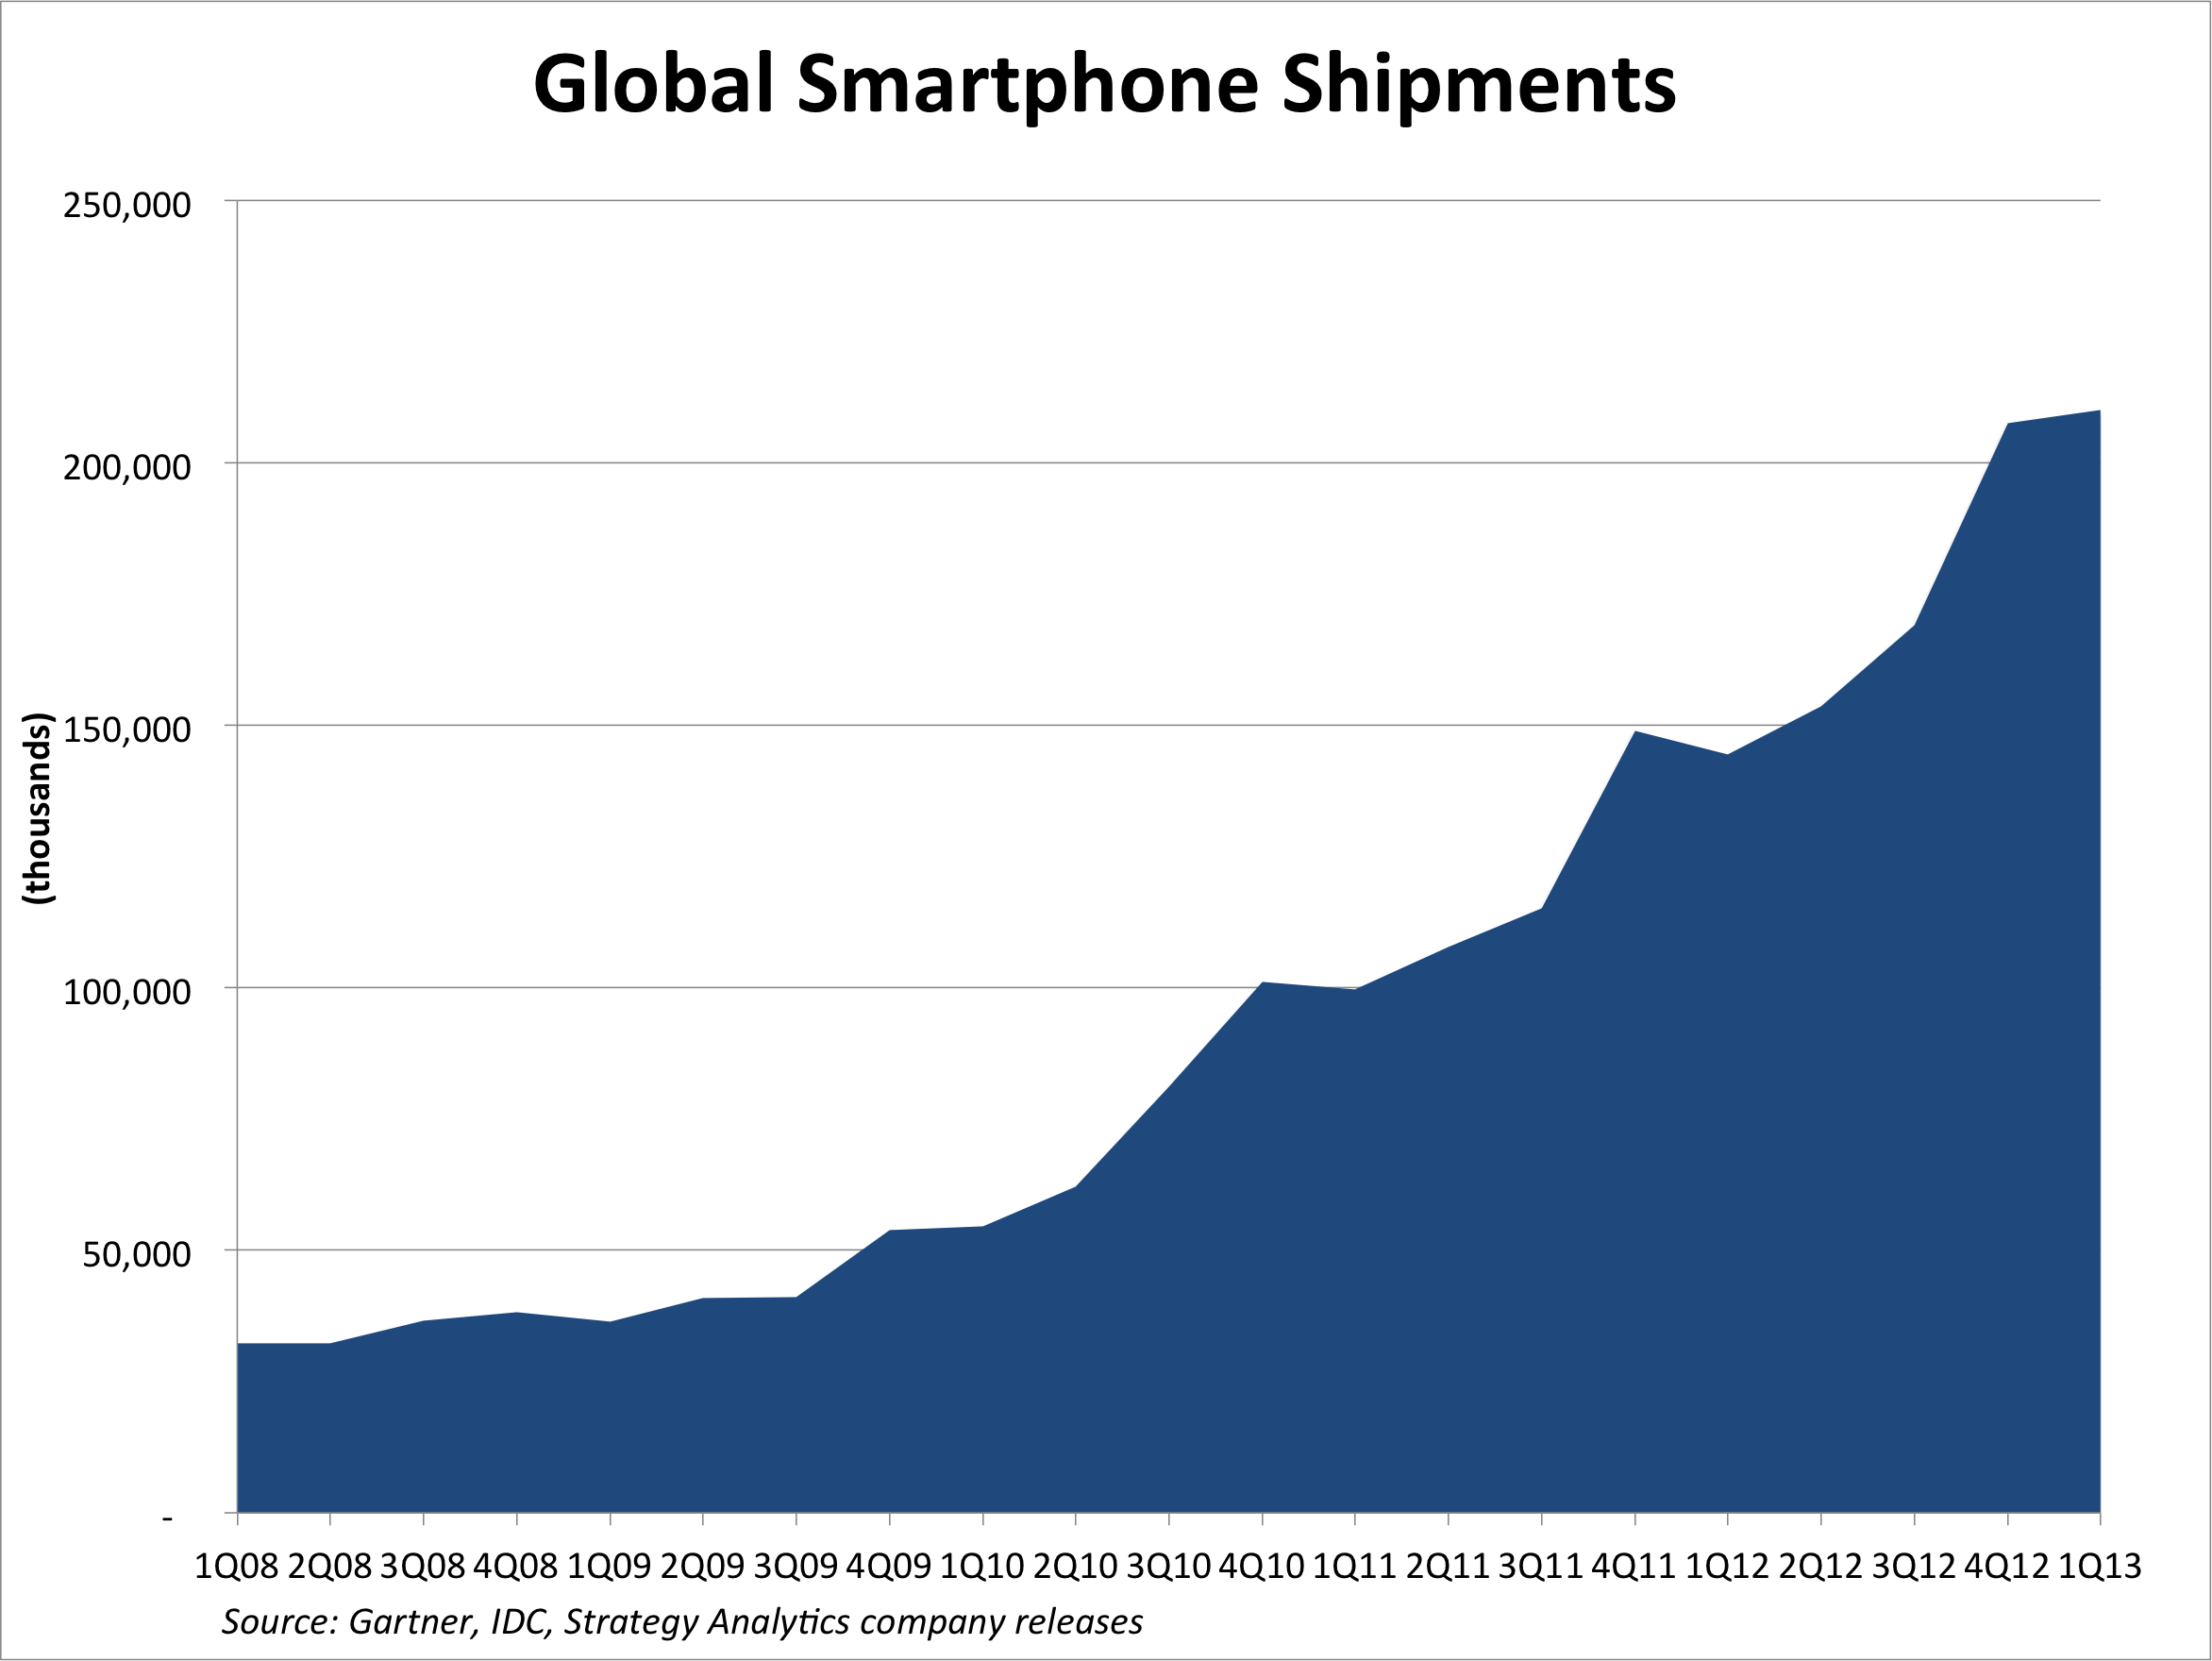
\includegraphics[height=46mm]{imagenes/capitulo1/img1.png}
	}
	\subfloat[Distribución mundial]{
	          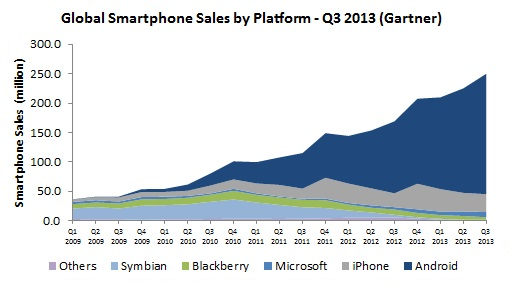
\includegraphics[height=46mm]{imagenes/capitulo1/img3.jpg}
	}

	\subfloat[Distribución en EEUU]{
	          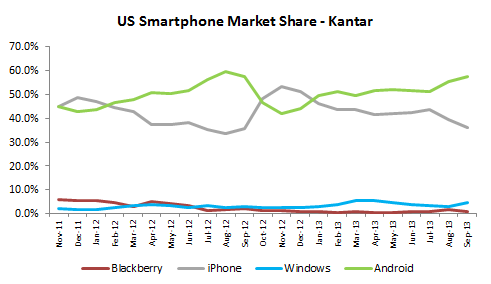
\includegraphics[height=42mm]{imagenes/capitulo1/img4.png}
	}
	\subfloat[Distribución en España]{
	          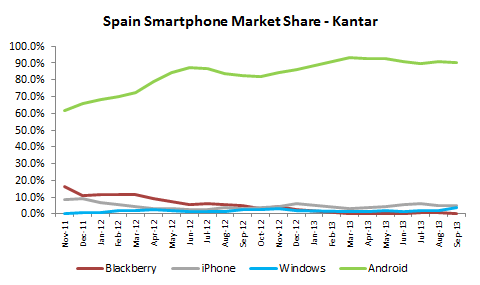
\includegraphics[height=42mm]{imagenes/capitulo1/img2.png}
	}
	\caption{Situación actual de los smartphones}
\end{figure}

Al observar en la gráfica ``a'' de la figura 1.1, podemos ver que el número de ventas de móviles se incrementan año tras año. Debido a su alto coste, la estrategia de mercado se está centrando en desarrollar este tipo de dispositivo low-cost, con un menor coste, para que estén al alcance de todos los bolsillos. El objetivo de esta estrategia es doblar la venta de smartphones de bajo presupuesto de forma anual hasta 2016, pasando de 4 millones de unidades en el año 2010 a unas 311 millones 6 años después.
\newline

En el resto de los gráficos de la figura 1.1 se muestra la distribución de las principales plataformas ejecutadas en los smartphones a nivel mundial, en Estados Unidos y en España. Cabe destacar que la plataforma Symbian, de Nokia, ha desaparecido casi por completo. A nivel mundial es un mercado dominado por Android. Ocurre lo mismo en España pero en Estados Unidos comparte el mercado junto con iPhone.
\newline

Tras realizar un pequeño análisis de las dos plataformas dominantes, se ha llegado a las siguientes conclusiones:
\begin{itemize}
\item Tanto Android como iPhone ofrecen un marco de trabajo en una primera fase estable y suficientemente evolucionado para el desarrollo de un proyecto de fin de carrera.
El desarrollo sobre IPhone implica unos gastos superiores respecto a Android debido a temas de licencias, coste del dispositivos y software necesario.
\item El tiempo requerido en el desarrollo sobre un IPhone es menor que en Android. Esta diferencia radica en que IPhone esta soportado en un pequeño conjunto de dispositivos muy reducido, tan sólo los productos ofrecido por la compañía Apple, mientras que en Android existen una gran variedad de  dispositivos con características dispares.
Por este motivo, un programa desarrollado en Android ha de ser probado en un mayor número de dispositivos móviles, lo que conlleva un mayor tiempo de pruebas.
\item El precio de un dispositivo móvil con un sistema Android y las características de aceleración gráfica 3D por hardware, están dentro del presupuesto personal  del proyecto.
\end{itemize}

\begin{figure}[h]
	\centering
        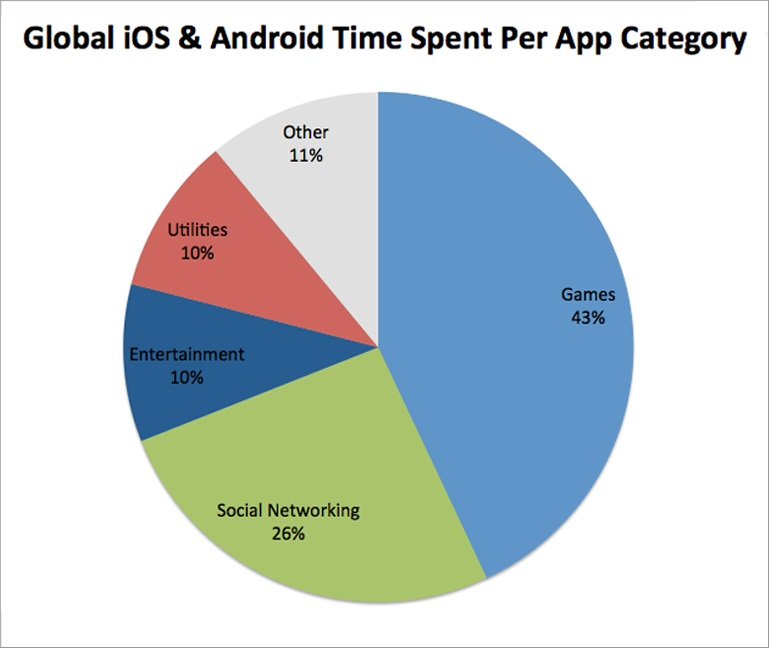
\includegraphics[height=55mm]{imagenes/capitulo1/img5.jpg}
	\caption{¿Para qué usamos los smartphones?}
\end{figure}

La situación descrita suscita un interés especial en adquirir un mayor conocimiento en el desarrollo de aplicaciones para smartphones Android. En la figura 1.2 se muestran un diagrama con las facetas en las que más tiempo empleamos cuando manejamos un smarthpone, lo que nos da una idea de las aplicaciones típicas en un dispositivo de estas características. 
\newline

Hemos de destacar el gran porcentaje de tiempo que dedicamos jugando con el smartphone, lo que justifica que el desarrollo de videojuegos se está convirtiendo en un nuevo nicho de mercado para las empresas. Actualmente existen varios framework de desarrollo de videojuegos con aspecto gráfico tridimensional para Android, el más famoso es Unity 3D. Sin embargo, esta situación era muy distinta cuando comenzó el proyecto, ya que no existía ningún framework o los que existían era muy precarios.
\newline 

Debido a la situación del mercado de los smartphone respecto a la creación de videojuegos con gráficos en 3D, surge en forma de proyecto de fin de carrera, la idea de dar respuesta a la pregunta que hizo que estudiara ingeniería informática años atrás, esa pregunta es:
\begin{center}
\texttt{¿Cómo se hace un videojuego?}
\end{center}

El juego elegido es Pacmania, una versión que simula las tres dimensiones y que la empresa Nanco desarrolló en 1988 basándose en una versión anterior en 2D llamada Pacman, conocida popularmente como comecocos. Se ha decidido implementar este videojuego ya que no existe ninguna versión parecida en Android, tan sólo una versión en 2D. En los siguientes gráficos podemos ver la versión actual para Android del juego Pacman junto con la versión de PC del juego Pacmania.

\begin{figure}[h]
		\centering
		\subfloat[Pacmania (PC)]{
		          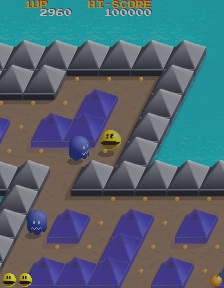
\includegraphics[height=6.5cm]{imagenes/capitulo1/PacmanPC.jpg}
		}
		\subfloat[Pacman (Android)]{
		          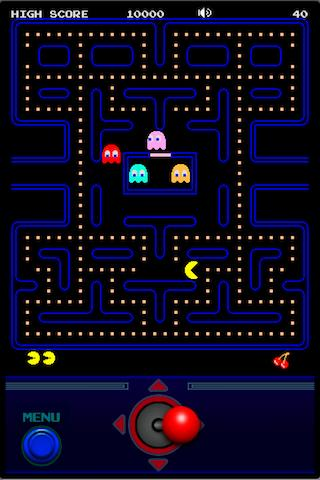
\includegraphics[height=6.5cm]{imagenes/capitulo1/PacmanAndroid.jpg}
		}
\end{figure}
	

\section{Evolución de los videojuegos}

La evolución de los videojuegos puede ser vista desde dos prismas bien diferenciados. Podemos hablar de cómo se han ido adaptando los formatos con los cuales se presentan al mercado, por ejemplo en máquinas recreativas, consolas\ldots\ Otra forma de ver esta evolución es centrándonos en las características de los videojuegos como por ejemplo el aspecto visual, conectividad\ldots\ 
\newline

A continuación vamos a detallar la evolución desde ambos puntos de vista, no sin antes mencionar un aspecto a tener en cuenta. Un cambio de formato puede tener implicaciones directas sobre las características del videojuego, por ejemplo, la diferencia de capacidad de procesamiento entre consolas y dispositivos móviles conlleva una perdida de calidad gráfica.
\newline

\subsection{Evolución de los formatos}

Actualmente el concepto de videojuego ha sido asimilado por la sociedad, cualquiera sabe qué es un videojuego, incluso han dejado de ser un producto exclusivo para adolescentes. Si nos remontamos a la década de los 40, la palabra videojuego aún no existía. En esta década se crean las primeras computadoras de la historia como Zuse, Colossus y ENIAC\ldots\ pero fue en 1949 cuando el laboratorio de Matemáticas de la Universidad de Cambridge presenta EDSAC, una computadora que no sólo se utilizó para realizar cálculos matemáticos. En 1952 Alexander S. Douglas construye sobre ella el videojuego Nought and Crosses, también llamado OXO. En España dicho juego es conocido como las tres en raya y permitía enfrentar a un jugador humano contra la máquina, visualizando el tablero sobre una pantalla de tubo de rayos catódicos.
\newline

\begin{figure}[!h]
	\centering	
	\subfloat[OXO]{
	          
\includegraphics[height=45mm]{imagenes/capitulo1/oxo.jpg}
	}
	\subfloat[Tennis for two]{
	          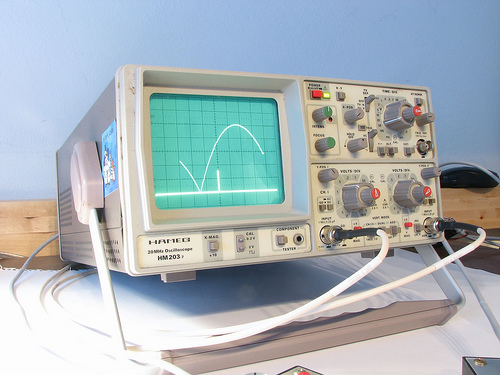
\includegraphics[height=45mm]{imagenes/capitulo1/tennis4two.jpg}
	}
	\caption{Los primeros videojuegos caseros que se crearon}
\end{figure}

En 1958, Will Higinbothamen en el laboratorio nacional de Brookhaven, simuló en un osciloscopio un partido de tenis. No estaba dotada de ningún tipo de inteligencia por lo que no se podía jugar contra la máquina y se necesitaban dos jugadores. Cada uno de ellos manejaba una especie de mando que tenía una pequeña rueda para indicar el ángulo de golpeo y un botón para golpear la pelota con una raqueta invisible. 
\newline

En 1961 unos estudiantes del Instituto de Tecnológico de Massachusetts (MIT), Steve Russell entre ellos, construye SpaceWar, un videojuego donde dos naves espaciales y armadas tenían que destruirse mientras evitaban la fuerza gravitatoria de una estrella. Tras pasarse horas jugando a SpaceWar, en 1971 Rusell finalmente decidió comercializarlo con el nombre ``Computer Space'', lo que dio origen a la primera máquina recreativa. 
\newline

Sin embargo, la difusión en el mercado de Computer Space fue mucho menor que PONG de Atari, la cual simulaba el juego del ping-pong. Esta segunda máquina recreativa salió al mercado un año más tarde, pero debido a que su difusión fue mucho mayor es considerada como la primera máquina recreativa. 
\newline

\begin{figure}[h]
	\centering	
	\subfloat[Pong]{
	          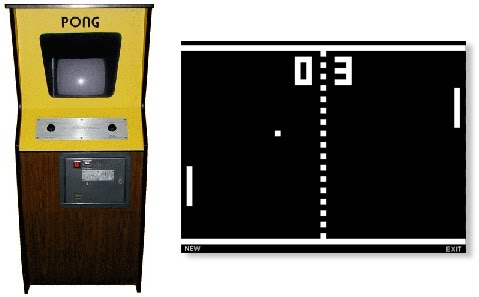
\includegraphics[height=45mm]{imagenes/capitulo1/Pong.jpg}
	}
	\subfloat[Computer Space]{
	          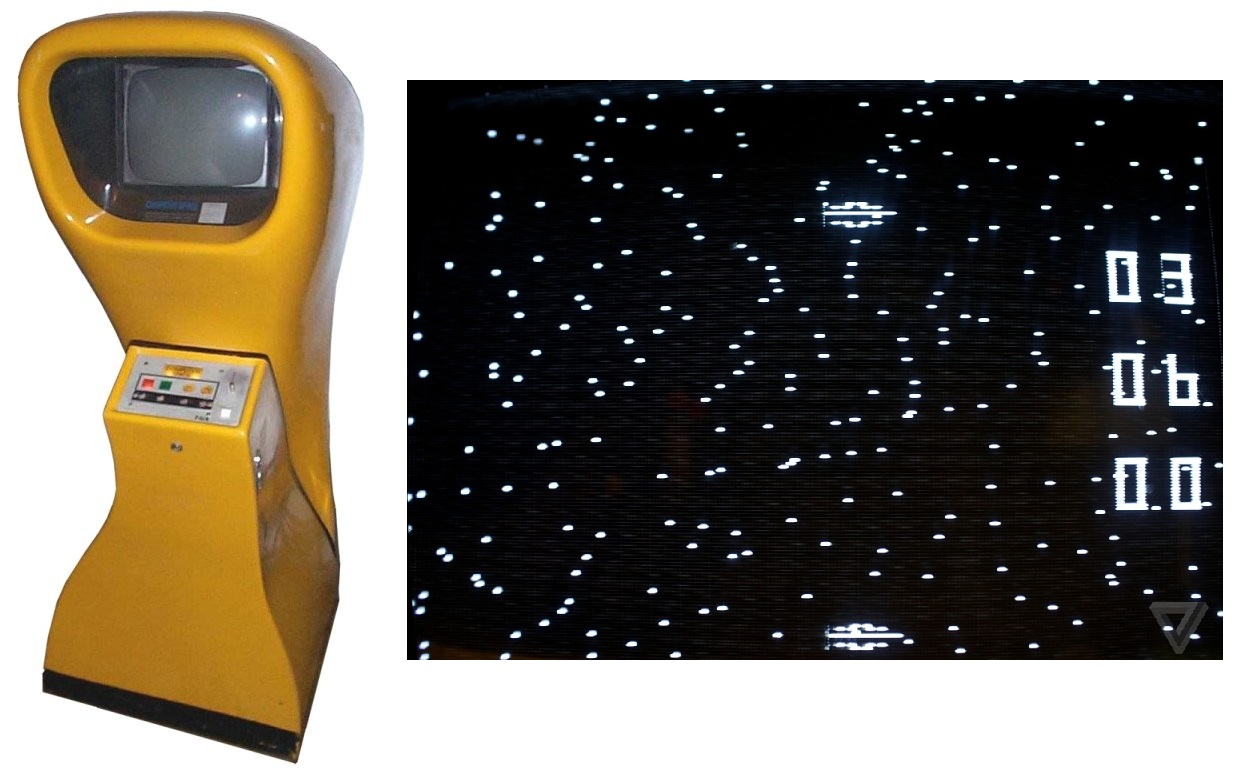
\includegraphics[height=45mm]{imagenes/capitulo1/ComputerSpace.jpg}
	}
	\caption{Los primeras máquinas recreativas}
\end{figure}

Pronto surgieron nuevas máquinas recreativas, algunas de ellas son King Kong, Pacman, Tetris, Super Mario Bros\ldots\ Los adolescentes acudían a un nuevo tipo de negocio, los salones recreativos, donde insertando una moneda podían jugar una partida al videojuego deseado. Este fue el comienzo de la industria de los videojuegos. 
\newline 

Con el trascurso de los años, fueron evolucionando en las temáticas, el aspecto visual y se hicieron más interactivos con la inclusión de nuevos periféricos como volantes, guitarras, cámaras que detectan el movimiento, etc. 
\newline 

En 1972 la industria de los videojuegos daba sus primeros pasos en los hogares con la creación de las primera generación de consolas. Un gran salto que  trasladaba la diversión de los salones recreativos al salón de casa. 
\newline
A continuación se muestra una tabla con las principales consolas que han salido al mercado y a que generación pertenecen.

\begin{figure}[h]
	\centering
         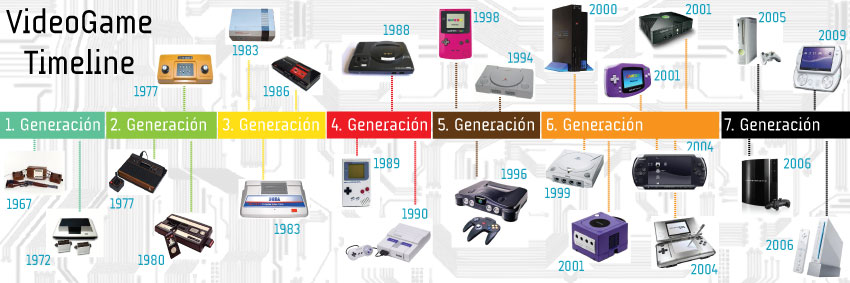
\includegraphics[width=14cm]{imagenes/capitulo1/consolas.jpg}
\end{figure}

Durante las distintas generaciones de consolas han existido intentos, con mayor o menor acierto, de hacerlas portátiles, ejemplo de ello son la GameBoy y la Nintendo DS, pero han sido los dispositivos móviles los que han logrado llevar los videojuegos a cualquier lugar en el que nos encontremos.
\newline

Google, con su plataforma Android, y Apple, con IPhone, son las firmas que lideran esta revolución tecnológica hacia un mundo móvil. Ambas por políticas empresariales bien distintas y exitosas. Google está más interesado en desarrollar sistemas abiertos y Apple genera productos cerrados. 

\subsection{Evolución de los características}

¿Qué es lo primero que nos llama la atención de un videojuego? El primer contacto que tenemos con un videojuego es su \textbf{aspecto visual} o gráficos. Apreciamos el nivel de detalle con el que son representados los paisajes, personajes y objetos. Inicialmente los gráficos eran minimalistas debido a la falta de procesamiento de los soportes, lo que conllevaba representar todo mediante cuadrados de escasos colores. Por este motivo podemos decir que existe una relación directamente proporcional entre capacidad de procesamiento y el aspecto visual. Al aumentar el número de cálculos matemáticos que se pueden realizar por segundo, podemos mejorar el nivel de detalle de lo representado en pantalla.
\newline

 El cambio más significativo ha sido la capacidad de poder reproducir modelos tridimensionales, dando la posibilidad de crear efectos visuales que simulan el movimiento de una cámara en un escenario.
\newline 

\begin{figure}[h]
	\centerfloat	 
	\subfloat[Internation Soccer]{
	          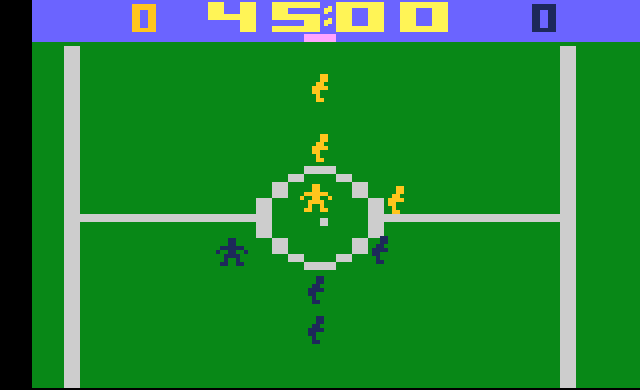
\includegraphics[height=40mm]{imagenes/capitulo1/evofutbol1.png}
	}
	\subfloat[Gol! '92]{
	          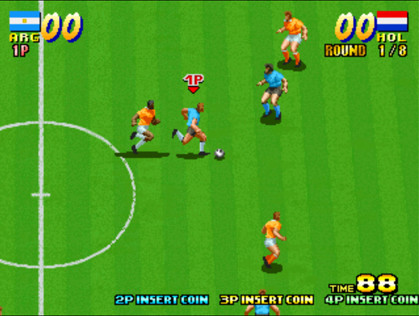
\includegraphics[height=40mm]{imagenes/capitulo1/evofutbol2.jpg}
	}
	\newline
	\subfloat[PES 2012]{
	          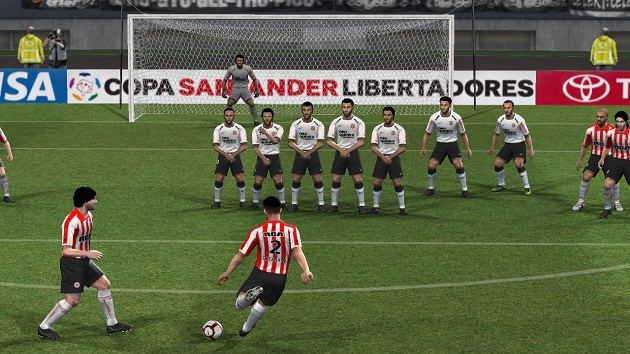
\includegraphics[height=45mm]{imagenes/capitulo1/evofutbol3.jpg}
	}
	\caption{Evolución gráfica en los videojuegos de fútbol}
\end{figure}

Ahora que el videojuego ha captado nuestra atención gráficamente, prestamos atención a la trama que se va entrelazando según avanzamos en él. En los primeros videojuegos la \textbf{historia} desarrollada era nimia pero, poco a poco, éste factor ha ganado importancia, hasta el punto en el cual podemos decir que los costes de desarrollo de un videojuego son equiparables al de una película.
\newline

Existe una característica que pasa desapercibida por el jugador al interiorizarla como algo natural. Estamos hablando de las  \textbf{propiedades físicas} del escenario en el cual nos movemos. El jugador no se para a pensar porqué el personaje que está manejando puede saltar, puede coger otros objetos pero no puede atravesar las paredes. Sin embargo, cuando la física del videojuego no funciona a la perfección, como por ejemplo cuando se atraviesan ligeramente ciertos objetos, no ve el agua de un rio fluir o las llamas del fuego no se mueven, son captadas por el usuario como fallos de importancia. Al igual que el aspecto gráfico de un videojuego, la física esta relacionada con la capacidad de procesamiento. Hoy en día podemos ver juegos que aplican algoritmos para calcular cómo han de moverse los elementos sólidos y fluidos, dando un gran realismo a los juegos.
\newline 

En el transcurso del videojuego podemos encontramos frente a otros personajes, que se relacionan en el escenario, como si fueran manejados por terceras personas. Es la \textbf{inteligencia artificial} la responsable de este comportamiento, que maneja personajes dotándoles de un comportamiento natural, como por ejemplo que un perro persiga y ladre a un extraño o que la gente de tu alrededor te mire si rompes algo. 
\newline

Es sorprendente la evolución de la inteligencia artificial, al principio los movimientos de los personajes podrían catalogarse de burdos y hoy en día nos hace dudar si tras un personaje se encuentra una persona o no.
\newline

Una de las preguntas habituales que todos nos hacemos de forma natural es cómo compartir las experiencias. Existen videojuegos en los cuales no es posible, en otros puede haber varios jugadores simultáneos. Al principio para que se pudiera dar esta situación, había que estar en la misma sala, sin embargo esta limitación desapareció debido a la \textbf{conectividad} de los soportes a través de Internet. Esta característica ha llevado a los videojuegos a un nuevo nivel convirtiéndolos en un acto social.

\subsection{Videojuegos en dispositivos móviles}

Una vez descrita la evolución de los videojuegos, tanto a niveles de formatos como características, se van a describir las implicaciones en el ámbito de los smartphone. 

\begin{figure}[h]
	\centerfloat	 
	\subfloat[Apalabrados]{
	          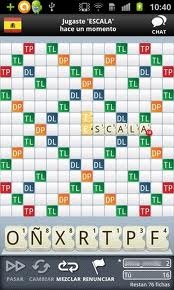
\includegraphics[height=60mm]{imagenes/capitulo1/apalabrados.jpg}
	}
	\subfloat[Angry Birds]{
	          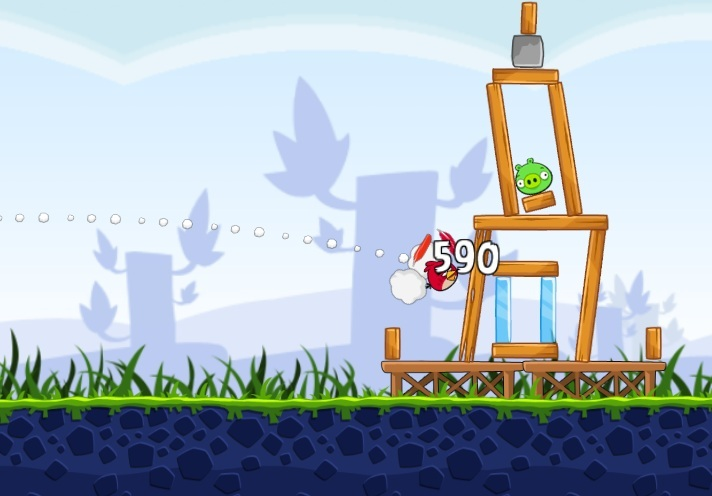
\includegraphics[height=50mm]{imagenes/capitulo1/angrybirds.jpg}
	}
	\subfloat[Candy Crush Saga]{
	          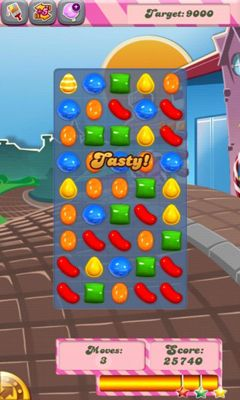
\includegraphics[height=60mm]{imagenes/capitulo1/candycrush.jpg}
	}
	\caption{Top éxitos en Android}
\end{figure}

A pesar de la gran evolución de los móviles, su capacidad de procesamiento no es, ni de lejos, comparable con las computadoras de sobremesa ni consolas. A esta situación se le suma un mercado emergente y que no dispone de frameworks especializados para el desarrollo de videojuegos, lo que ha provocado una involución en casi todas sus características.
Este hecho puede constatarse al consultar los videojuegos más descargados para Android. Predominan los juegos sin una historia desarrollada y con un aspecto visual simplista. Alguno de ellos son Apalabrados, Candy Crush Saga y Angry Bird, de los cuales se muestran capturas de pantalla en la figura 1.6.
\newline

Un ejemplo de un videojuego que aprovecha el potencial de los smarthones actuales es el Grand Theft Auto, a pesar de ello, existe una gran diferencia en su aspecto gráfico en comparación con la versión de consola, tal y como muestran las siguientes capturas de pantallas.

\begin{figure}[h]
	\centerfloat	 
	\subfloat[Android/iPhone]{
	          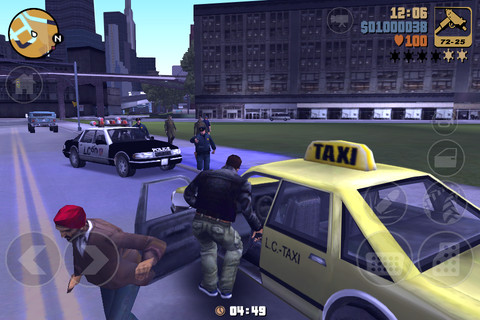
\includegraphics[height=45mm]{imagenes/capitulo1/GTA3.jpg}
	}
	\subfloat[Play Station 3]{
	          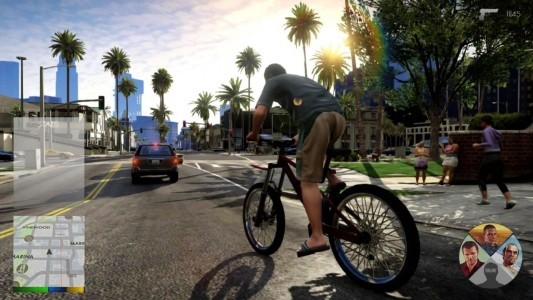
\includegraphics[height=45mm]{imagenes/capitulo1/GTAV.jpg}
	}
	\caption{Grand Theft Auto}
\end{figure}

Una dificultad añadida consiste en la desaparición del teclado y mandos con los que controlar el videojuego, siendo sustituida en la mayoría de los casos por la pantalla táctil o lo sensores de movimiento del dispositivo. 
\newline

Hay que destacar que un smartphone ofrece un serie de características adicionales propias de ellos, la más destacables son el GPS y la cámara. De estas cualidades han surgido dos conceptos nuevos:
\begin{itemize}
\item La \textbf{movilidad} permite a las aplicaciones mejorar su funcionamiento al poder incluir la posición en la que nos encontramos. Por ejemplo, nos permite saber cúal es la estación de metro más cercana o hacer campañas publicitarias por proximidad.
\item La \textbf{realidad aumentada} permite mezclar el mundo real y el digital a través del uso de la cámara. Por ejemplo, podríamos ver como nos queda un mueble en un salón a través de la cámara.
\end{itemize}

\begin{figure}[h]
	\centerfloat	 
        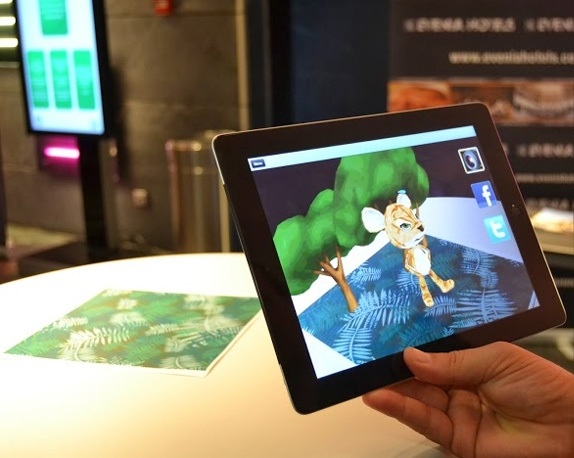
\includegraphics[height=45mm]{imagenes/capitulo1/realidadaumentada.jpg}
	\caption{Ejemplo de realidad aumentada}
\end{figure}

Éstas particularidades están estimulando la creación de otros tipos de videojuegos, como por ejemplo Ingress, de Google. Este videojuego consiste en salir a la calle con el móvil, abrir la aplicación y buscar  \emph{fuentes de esta misteriosa energía} ocultas en nuestra ciudad, transformando el mundo real en el escenario del videojuego mediante el uso de las la cámara, las redes de telefonía y el GPS. 
%\newline
%
%Visto desde perspectivas comerciales, este tipo de videojuegos pueden ser utilizados para recoger una cantidad ingente de información de %geoposicionamiento, la cúal puede ser utilizada para mejorar Google Maps con la ayuda de todos.

\section{Objetivos del proyecto}

Una vez explicadas las motivaciones que han dado lugar al proyecto de fin de carrera, la evolución de los videojuegos y la implicaciones que existentes en smartphone, se van a definir los objetivos del proyecto.

\begin{enumerate}
\item Adquirir los conocimientos específicos necesarios para poder desarrollar videojuegos con modelos en 3D.
\item Aprender a realizar diseños gráficos con Blender para generar el aspecto gráfico de los elementos de un videojuego.
\item Aprender el lenguaje de programación específico para tarjetas gráficas llamado GLSL (OpenGL Shading Language).
\item Conseguir los conocimientos del desarrollo de aplicaciones en Android.
\item Comprar un smarthpone adecuado para el desarrollo del proyecto que cuente con el hardware que permita aceleración gráfica mediante OpenGL ES 2.0 y la versión Gingerbread de Android. Estos conceptos son desarrollos en la primera parte del proyecto. Tras realizar un estudio de mercado de los smarthpone que cubrían esta características, el móvil elegido fue el HTC Desire.
\item Desarrollar una librería genérica que facilite el desarrollo de videojuegos para Android. La llamaremos TfcGameEngine y contendrá diversas funcionalidades:
	\begin{itemize}
	\item Bucle principal del videojuego en el cual se van secuenciando imágenes como si de una película se tratase.
	\item Soporte para OpenGL ES 2.0 (Este concepto que se explicará en el capítulo 3 del proyecto).
	\item Utilidades para el cálculo de movimiento en función del tiempo, velocidad y aceleración, es decir, cinemática.
	\item Detección de colisiones entre elementos del juego.
	\item Algoritmos que permitan desplazar los personajes de videojuego sobre la escena de forma manual, aleatoria o entre dos puntos.
	\item Procesamiento de los diseños gráficos realizados con Blender.
	\item Motor de música que permita reproducir melodías y efectos de sonido.
	\end{itemize}

	Un principio básico que ha primado en el diseño de la librería es que tiene que ser fácilmente extensible por terceros, permitiendo de esta forma, añadir nuevas funcionalidades. 

\item Realizar una prueba de concepto de dicha librería programando un videojuego de un comecocos en 3D, llamado Pacmania. Este juego consiste en controlar al Pacman, un personaje que ha de recoger las pastillas de un escenario custodiado por fantasmas. Para ello será necesario:
	\begin{itemize}
	\item Realizar los diseños gráficos de los escenarios y personajes del videojuego, que son dos escenarios, un fantasma y un pacman.
	\item Realizar un proceso de carga de los ficheros contenidos en un directorio de configuración. Este directorio contiene los escenarios, personajes, efectos especiales, melodías, vídeos, etc.
	\item Ampliación de la librería TfcGameEngine para incluir la lógica especifica del videojuego como por ejemplo, controlar la puntuación y número de vidas de la partida.
	\item Creación de animaciones con la cámara cuándo comienza un nivel o el Pacman es capturado por un fantasma.
	\item Reproducción de efectos especiales y melodías.
	\item Pantalla de configuración que permita indicar si el sonido esta activo y donde se encuentra el directorio de configuración.
	\item Registro de las mejores puntuaciones en una base de datos SqlLite.
	\end{itemize}
\item Testar el videojuego en otros smartphone como Galaxy S2 y Nexus 5.
\end{enumerate}

Para mas información sobre la librería TfcGameEngine y el juego Pacmania, consultar los catálogo de requisitos del capítulo 5. 

\part{Conocimientos previos}
 \chapter{Android}

Una vez enmarcado el proyecto sobre la plataforma Android, en este capítulo se pretende dar una vista más especifica de las funcionalidades que nos ofrece en cada una de sus versiones. Se explicará cómo surgió esta plataforma y los conceptos básicos de cómo están compuestas sus  aplicaciones y el entorno de desarrollo necesario para crearlas y distribuirlas.
\newpage

\section{El origen}

El germen de Android nace en el proyecto Paradigm, de la empresa General Magic, en el año 1990. Esta empresa surgió de Apple y su objetivo fue crear un sistema operativo para teléfonos móviles al que llamarían Magic Cup. El proyecto fracasó pero uno de sus arquitectos continuó su carrera profesional en Artemis Reseach, que posteriormente comprada por Microsoft. Más tarde fundó Danger Inc, también comprada por Microsoft y que abandonó para formar una  nueva empresa llamada Android Inc, que fue vendida a Google en el año 2005. El arquitecto del que estamos hablando es Andy Rubin, actual vicepresidente de Google. 
\newline

En 5 de Noviembre del 2007, se funda la Open Handset Alliance, dirigida por Google junto con unos 34 miembros más, entre los que se incluían fabricantes de dispositivos móviles, desarrolladores de aplicaciones, algunos operadores de comunicaciones, fabricantes de chips\ldots\ anunciando la creación de una plataforma de código libre para teléfonos móviles. 
\newline

El 23 de septiembre de 2008, nace la primera versión de lo que hoy se conoce como Android y un mes más tarde sale al mercado HTC Dream (T-Mobile G1) el primer móvil con Android. 

\begin{figure}[ht]
\centering
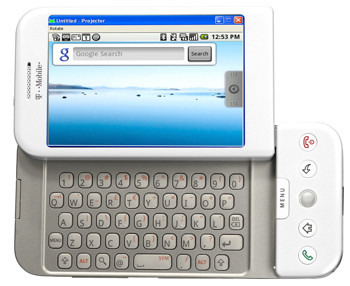
\includegraphics[height=8cm]{imagenes/capitulo2/htc-dream.jpg}
\caption{HTC Dream}
\end{figure} 


\section{Arquitectura}

Android es una plataforma para smartphones, pero ha evolucionado hacia otro tipo de dispositivos móviles como las tabletas. En el siguiente gráfico se muestra la estructura general de esta plataforma:
\begin{figure}[ht]
\centering
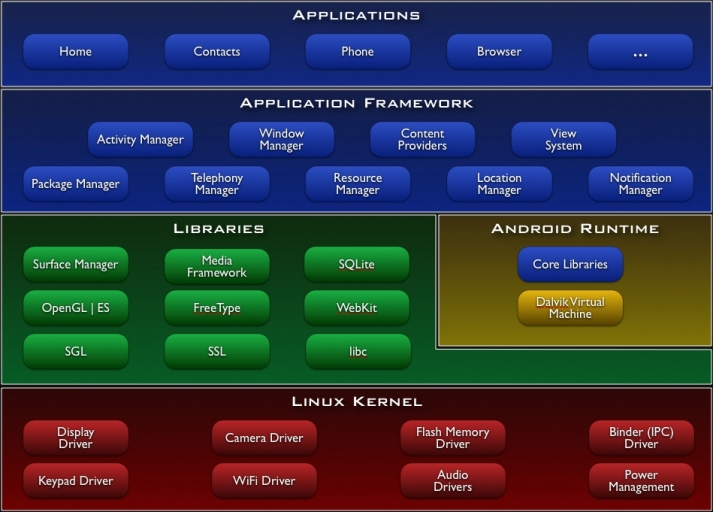
\includegraphics[height=9cm]{imagenes/capitulo2/androidArchitecture.jpg}
\caption{Arquiectura Android}
\end{figure} 

\begin{description}
\item [Un sistema operativo Linux,] responsable de gestionar los recursos ofrecidos por el hardware como memoria, batería, pantalla\ldots\ Cada fabricante ofrece distintos drivers para comunicarse con su hardware y es el sistema operativo quien nos independiza de tener que conocer cada una de ellas, 
ofreciéndonos una interfaz común. También es el responsable de gestionar los distintos recursos que ofrece el dispositivo como son:
\begin{multicols}{2}
\begin{itemize}
\item Pantalla
\item Teclado
\item Cámara de fotos
\item Wifi
\end{itemize}
\begin{itemize}
\item Memorias flash
\item Audio 
\item Batería
\item etc
\end{itemize}
\end{multicols}

\item [Librerías en C y C++] que permiten acceder al hardware del dispositivo móviles u otros componentes que estén integrados. Las librerías principales se listan a continuación:
\begin{itemize}
\item Surface Manager: gestiona los gráficos mostrados en pantalla.
\item Media Framework: permite reproducir imágenes, audio y vídeo. 
\item SQLite: gestiona el acceso a bases de datos relacionales. 
\item WebKit: navegador web optimizado.  
\item SGL: permite realizar gráficos en 2D.  
\item OpenGL ES: permite realizar gráficos en 3D.
\item FreeType: procesamiento de imágenes vectoriales.
\end{itemize}

\item [Entorno de ejecución,] con la máquina virtual basada en Java llamada \textbf{Dalvik}, que ha sido modificada para optimizar entornos con restricciones de procesamiento, memoria y espacio, como son los dispositivos móviles. 

Dalvik permite independizar las aplicaciones del hardware mediante ficheros con un formato con extensión \textbf{dex}, que significa Dalvik executable. 

El programador utilizará la sintaxis Java y dispondrá de un amplio conjunto de JME\footnote{Java Micro Edition: Librería Java para el desarrollo de aplicaciones móviles}, optimizado para Dalvik. Al compilar el código se generarán bytecode de java, que posteriormente es optimizado mediante la herramienta dx, para que optimice el código y genere el fichero dex. 

La comunicación del entorno de ejecución con las librerías en C y C++ se realiza mediante JNI\footnote{Java native interface: Interfaz nativo de java}.

\item [Framework de aplicaciones,] ofrece la funcionalidad básica de Android, siendo las más destacables:
\begin{itemize}
\item Activity Manager: gestiona las actividades que se están ejecutando en el smarthpone. Toda aplicación en Android está compuesta por actividades y se define como un componente gráfico con su propio ciclo de vida. En la siguiente sección veremos en detalle la composición las aplicaciones en Android.
\item Windows Manager: gestiona qué es lo que se visualiza por pantalla. Cuando una actividad necesita ser visualizada por el usuario, ha de invocar a este componente.
\item Contents Provider:  gestiona grupos de información que son utilizados por varias aplicaciones. Los principales contenidos de Android son la agenda de contactos y el calendario.
\item Telephony Manager: permite acceder a las funcionalidades de telefonía del dispositivo, protocolos de comunicación permitidos, los datos de la SIM, estado de la conexión\ldots
\item Resource Manager: permite acceder al contenido estático de la aplicación, como ficheros de audio, XML de configuración\ldots
\item Location Manager: permite acceder a la información de localización del dispositivo por GSP, WIFI y las torretas de telefonía.
\item Notification Manager: permite acceder al componente de notificaciones de Android, un panel donde se registran avisos de distinta índole, por ejemplo, nuevos mensajes, llamadas perdidas, actualizaciones\ldots
\end{itemize}

\item [Otras aplicaciones] son instaladas en el dispositivo por las compañías u los usuarios de los dispositivos móviles. La forma más común en la que estás aplicaciones pueden ser instaladas es desde la web de Google. Inicialmente surgió con el nombre de Google Market y posteriormente fue renombrado como Google Play. \begin{center}\texttt{https://play.google.com}\end{center}
\end{description}


\section{Entorno de desarrollo}

El siguiente paso, tras haber tomado conciencia sobre qué es Android, es explicar las herramientas principales que nos ofrece la plataforma para facilitar el desarrollo de aplicaciones:

\begin{description}
\item [Eclipse,] un IDE\footnote{Integrated developement Environment: aplicación compuesta por un conjunto de herramienta para el desarrollo de aplicaciones} desarrollado por la comunidad OpenSource, que se caracteriza por permitir ser configurado por terceros. 
\item [Android Developer Tools (ADT),] plugin que configura Eclipse para poder desarrollar aplicaciones en Android.
\item [Android Debug Bridge (ADB)] es una herramienta que permite conectarse vía USB con dispoistivos Android y realizar un conjunto de acciones sobre él. Las más utilizadas son instalar aplicaciones, mover ficheros o crear una sesión mediante el protocolo de telnet, accediendo directamente con el sistema operativo Unix del dispositivo móvil.
\item [Un emulador] que cubre gran parte de las características soportadas en dispositivos móviles con Android. Permite ejecutar aplicaciones sin necesidad de tener un dispositivo físico. 
\item [Android Virutal Device (ADV),] ficheros que definen la configuración hardware de un dispositivo móvil y son cargados en el emulador. Son generados mediante una herramienta llamada Android, integrada dentro de su entorno de desarrollo.
\item [Mksdcard,] herramienta que permite simular una tarjeta de memoria virtual sobre un fichero, la cual podrá cargarse dentro del emulador.
\item [Logcat,] herramienta que nos permite ver las trazas de información que van dejando todas las aplicaciones que se ejecutan en el dispositivo móvil.
\item [Otras herramientas] que permiten diversas funcionalidades para generar copias de seguridad, analizadores y ofuscadores de código\ldots\ 
\end{description}


\section{Estructura de una aplicación}

Una vez que tenemos montado nuestro entorno de desarrollo con las herramientas mencionadas en el apartado anterior, se explicará la estructura de una aplicación en Android. Al crear un proyecto, se generará la siguiente estructura de ficheros:
\begin{itemize}
\item \textbf{AndroidManifest.xml,} fichero principal de la aplicación donde se indican las características principales de la aplicación. Es obligatorio definir cuales son las actividades que componen la aplicación, cuál de ellas es la principal, la versión de la aplicación y versión requerida del SDK. Además se han de definir cuáles son los permisos necesarios para el correcto funcionamiento de la aplicación, por ejemplo envío automático de mensajes, acceso al GPS, contactos, cámara,  etc. Al instalar la aplicación, se indicará al usuario los permisos que requiere y ha de aceptarlos si desea instalarla.
\item Directorio  \textbf{src} donde se ubican las fuentes java. El proyecto creado con el plugin ADT, genera una clase llamada como el proyecto que extiende de Activity y será el punto inicial que se ejecutará en la aplicación.
\item Directorio \textbf{res} donde se ubican distintos recursos en una jerarquía de directorios en función de las características de los mismos:
\begin{itemize}
\item drawable-hdpi: contiene las imágenes de alta densidad.
\item drawable-mdpi: contiene las imágenes de media densidad
\item drawable-ldpi: contiene las imágenes de baja densidad.
\item layout: contiene ficheros xml con la definición de las interfaces gráficas que se cargarán en la actividad.
\item values: contiene ficheros xml donde se definen propiedades utilizadas por la aplicación como colores, cadenas de texto\ldots
\end{itemize}
\end{itemize}

Una aplicación Android puede estar compuesta por varias actividades, consideradas como unidades atómicas, buscando en ellas una alta cohesión y bajo acoplamiento. 
\newline 

Debido a las limitaciones del dispositivo móvil, las actividades son gestionadas por Android atendiendo a su estado y gestionarlas de la forma más eficiente posible.
\newline

Para comprender mejor el concepto de actividad, recurriremos al ejemplo principal de la página de desarrolladores de Android\footnote{http://developer.android.com}. El ejemplo \emph{Hello World} está compuesto por dos actividades, en la primera de ellas se solicita una cadena de texto y en la segunda se muestra la cadena con una letra mayor.  De forma coloquial, podemos entender las actividades como las distintas pantallas que componen una aplicación.

\begin{figure}[!h]
\centering
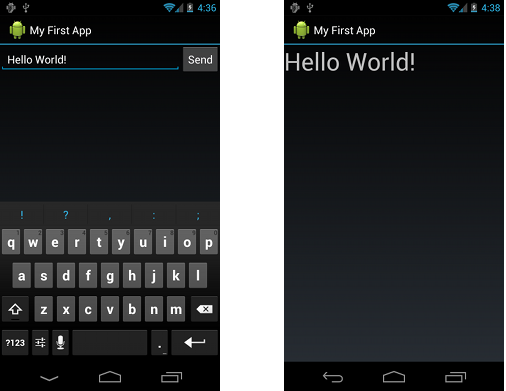
\includegraphics[height=8cm]{imagenes/capitulo2/firstapp.png}
\caption{Actividades del ejemplo Hello World}
\end{figure}

Toda actividad sigue un ciclo de vida, se van produciendo eventos que provocan una transición a un nuevo estado. Los eventos principales de este ciclo de vida son los siguientes:

\begin{itemize}
\item \textbf{onCreate:} Ocurre cuando la aplicación se crea. En este punto se ha de crear la interfaz gráfica e inicializar las estructuras de datos pertinentes.
\item \textbf{onStart:} Ocurre cuando la actividad se va a mostrar en pantalla por primera vez.
\item \textbf{onRestart:} Ocurre cuando la actividad parada va a mostrarse de nuevo.
\item \textbf{onResume:} La actividad comienza a visualizarse en pantalla, interactuando con el usuario.
\item \textbf{onPause:} La aplicación se ha pausado. Y deja de interaccionar con el usuario. En ese momento, todos los datos serán almacenados en la memoria secundaria, ya que el sistema puede terminar esta actividad pausada si se ve baja de recursos. Si se reactivara, pasaría al estado \texttt{onResume}.
\item \textbf{onStop:} Cuando una segunda actividad, nueva o reactivada, ha de mostrarse en pantalla. La actividad mostrada en esos momentos recibe este evento, pasando a un segundo plano, un estado candidato a ser destruido en caso de falta de memoria. Si la actividad pasase de nuevo al primer plano, cambiaría a estado \texttt{onRestart}.
\item \textbf{onDestroy:} La aplicación acaba y se destruye, bien porque acaba ella mima o el sistema la termina.
\end{itemize}

\begin{figure}[!h]
\centering
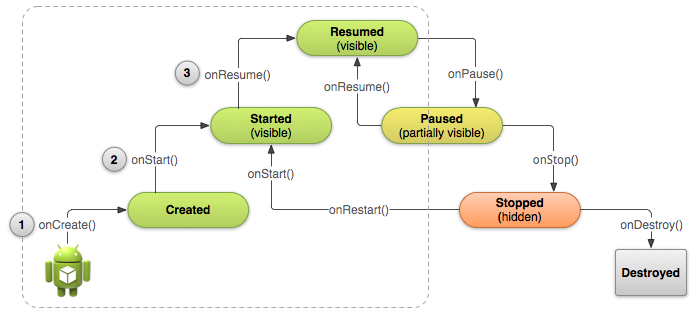
\includegraphics[height=5.8cm]{imagenes/capitulo2/activity_lifecycle2.png}
\caption{Ciclo de vida de una actividad}
\end{figure}

\section{Evolución}

Actualmente existen varias versiones de Android que van incorporando nuevas funcionalidades. La primera versión, llamada \textbf{Apple Pie} (Pastel de manzana), sólo se incorporo al modelo HTC-Dream\footnote{Para más información sobre las especificaciones hardware consulte los apéndices}.
\newline

Su característica más importante consistía en poder sincronizar los datos del móvil y la cuenta de Google. Otras  características a destacar son:
\begin{multicols}{2}
\begin{itemize}
\item HSDPA/850/900/1800/1900.
\item GPRS.
\item SMS y MMS.
\item Cámara de fotos.
\item Wifi (Cifrado WEP).
\item Bluetooth
\item USB 1.0
\item Navegador HTML 
\item Aplicación YouTube
\end{itemize}
\begin{itemize}
\item Aplicación música
\item Aplicación Android Market\footnote{Centro de descarga de aplicaciones para el móvil}
\item Aplicación de bloqueo táctil
\item Aplicación GMail
\item Aplicación Google Calendar
\item Aplicación Google Contacts
\item Aplicación Google Talk\footnote{Aplicación de intercambio de mensajes de texto}
\item Aplicación Google Maps

\end{itemize}
\end{multicols}

\begin{figure}[!h]
\centering
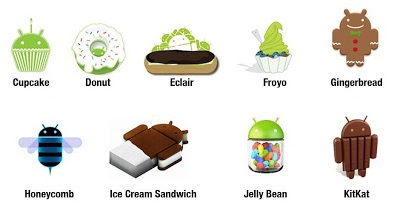
\includegraphics[width=13cm]{imagenes/capitulo2/android-versiones.jpg}
\caption{Logotipos de las versiones de Android}
\end{figure}
\subsection{Cupcake} 

El 30 de abril del 2009 se presenta la versión 1.5 de Android, conocida como Cupcake. Esta versión se caracteriza por:

\begin{itemize}
\item Estar basada en el kernel Linux 2.6.27.
\item Tener un teclado virtual, innecesario en la versión anterior ya que el HTC Dream tenía un teclado físico. 
\item Se mejora la velocidad de la cámara de fotos y se permite grabar vídeos.
\item Permite subir video y fotos a YouTube y Picassa.
\item Se mejorar el soporte bluetooth estéreo.
\item Se permite insertar nuevos widget desarrollados por terceros.
\item Transiciones de pantallas animadas.
\item Mejoras de tiempo de respuesta en el acceso GPS al utilizar A-GPS.
\item Mejorar el rendimiento en WebKit con el interprete de javascript \emph{SquirelFish}.
\item Posibilidad de cortar y pegar texto seleccionado.
\item Gestor de aplicaciones instaladas.
\end{itemize} 

\begin{figure}[!h]
	\centering	
	\subfloat[Teclado virtual]{
	          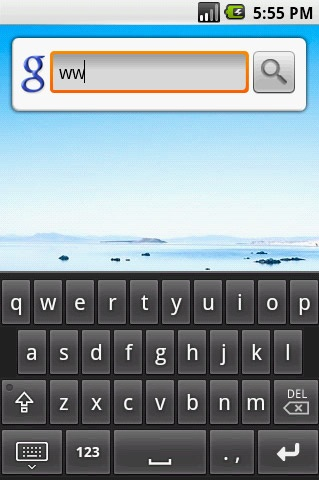
\includegraphics[height=7cm]{imagenes/capitulo2/cupcake-keyboard.jpg}
	}
	\hspace{0.8cm}
	\subfloat[Gestor de aplicaciones]{
	          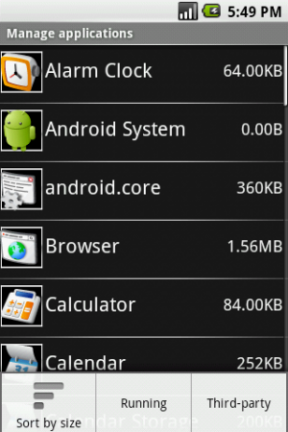
\includegraphics[height=7cm]{imagenes/capitulo2/cupcake-appmanager.png}
	}
	\caption{Novedades de la versión Cupcake}
\end{figure}


\subsection{Donut}

El 15 de Septiembre de 2009 se presenta la versión 1.6, conocida como Donut. Esta versión se caracteriza por:

\begin{itemize}
\item Soporte para telefonía de datos mediante CDMA.
\item Creación de redes virtuales mediante VPN.
\item Cifrado WAP en conexiones WiFi.
\item Motor de texto por voz que permite traducir un texto y escucharlo.
\item Nuevo applet de búsqueda que consulta tanto en Internet cómo en los datos del dispositivo.
\item Gestures que permite realizar acciones en el móvil al realizar una trazada con el dedo sobre la pantalla.
\item Soporte para pantallas de distintos tamaños y densidades.
\item Aplicación de gestión de batería por aplicación.
\end{itemize}

\begin{figure}[!h]
	\centering	
	\subfloat[Applet búsqueda]{
	          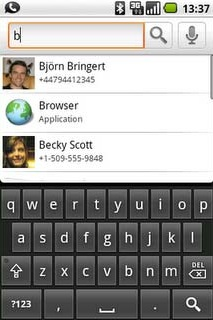
\includegraphics[height=7cm]{imagenes/capitulo2/donut-quicksearch.jpg}
	}
	\subfloat[Gestoures]{
	          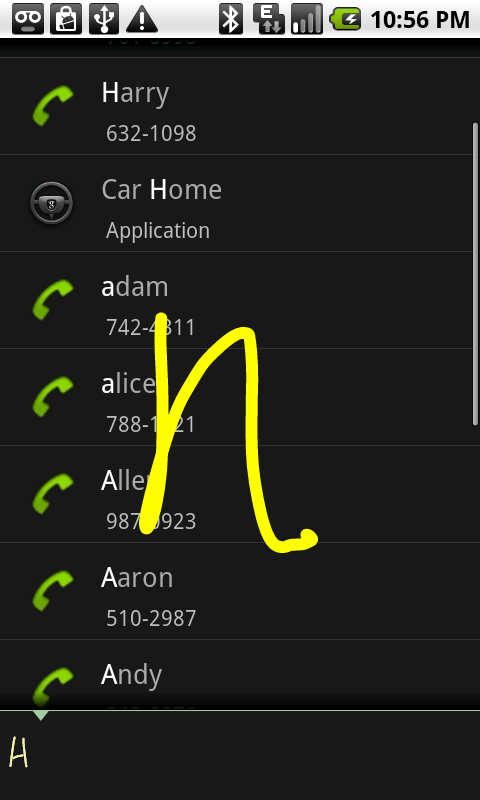
\includegraphics[height=7cm]{imagenes/capitulo2/donut-gestoures.png}
	}
	\subfloat[Gestor batería]{
	          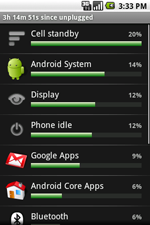
\includegraphics[height=7cm]{imagenes/capitulo2/donut-battery.png}
	}
	\caption{Novedades de la versión Donut}
\end{figure}

\subsection{Eclair} 

El 26 de octubre del 2009 se presenta la versión 2.0 de Android, conocida como Eclair. Esta versión se caracteriza por:

\begin{itemize}
\item Sincronización con Exchange.
\item Sincronización con multiples cuentas.
\item Soporte HTML 5.
\item Novedades en el uso de cámara que incluye flash, zoom digital\ldots
\end{itemize}

\subsection{Froyo} 

El 20 de mayo del 2010 se presenta la versión 2.2 de Android, conocida como Froyo. Esta versión se caracteriza por:
\begin{itemize}
\item Optimizaciones en velocidad,memoria y rendimiento.
\item Soporte Flash.
\item Instalación de aplicaciones en la SD en el almacenamiento interno de algunos dispositivos móviles.
\item Anclaje por USB, permitiendo al dispositivo al que se conecte el móvil usar la red de datos.
\item Soporte C2DM (Cloud to device Messaging) que permite sincronizar datos de una forma más efectiva. En vez de pooling es el servidor quien notifica al cliente que los datos han sido modificados.
\item Soporte OpenGL ES 2.0 para generación de gráficos tridimensionales.
\end{itemize}

\subsection{Gingerbread}

El 6 de diciembre del 2010 se presenta la versión 2.3 de Android, conocida como Gingerbread. Esta versión se caracteriza por:
\begin{itemize}
\item Aplicación Google Wallet para realizar pagos mediante móvil.
\item Soporte NFC (Near Field Communication). Esta tecnología permite comunicar de forma inalámbrica de corto alcance y alta frecuencia entre dispositivos para el intercambio de datos.
\item Soporte VoIP para realizar telefonía IP (Llamadas por Internet).
\item Mejora de rendimiento en el recolector de basura de Davilk.
\item Soporte nativos para sensores como el giroscopio y barómetro.
\end{itemize}

\begin{figure}[!h]
\centering
         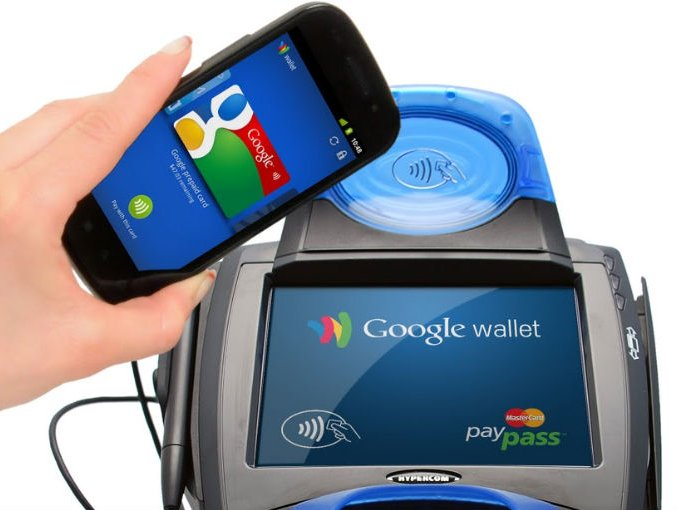
\includegraphics[height=6cm]{imagenes/capitulo2/gingerbreak-wallet.jpg}
	\caption{Google Wallet}
\end{figure}

\subsection{Honeycomb}

El 22 de febrero del 2011 se presenta la versión 3.0, conocida como Honeycomb. Esta versión consiste en una adaptación de la interfaz gráfica para tabletas. También se incluye un mayor soporte USB para conectar dispositivos a la tableta.

\begin{figure}[!h]
\centering
         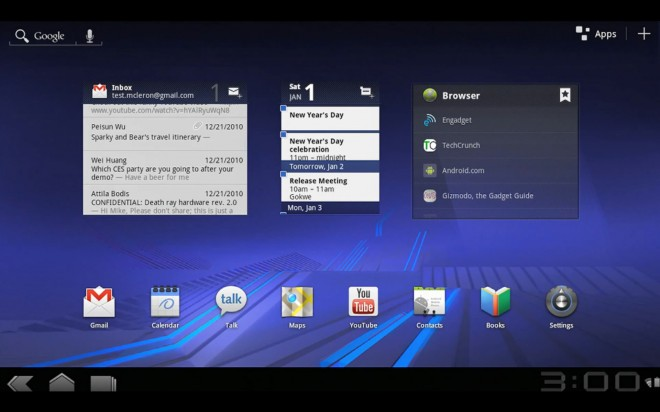
\includegraphics[width=10cm]{imagenes/capitulo2/honeycomb-screen.jpg}
	\caption{Nueva interfaz gráfica}
\end{figure}

\subsection{Ice Cream Sandwich}

El 19 de octubre del 2011 se presenta la versión 4.0 de Android, conocida como Ice Cream Sandwich. Esta versión unifica las dos anteriores, siendo tanto para móviles como para tabletas. Esta versión se caracteriza por:
\begin{itemize}
\item Se basa en el kernel 3.0.1 de Linux.
\item Soporte WiFi direct, que permite conectar dispositivos por WiFi sin necesidad de puntos de acceso.
\item Grabación de vídeos en FullHD.
\item Interfaz gráfica de usuario acelerada mediante hardware.
\item Aplicación Android Beam para intercambio de ficheros mediante NFC.
\item Desbloqueo facial.
\item Soporte para fotos panorámicas.
\item Barra multitarea que permite ver todas las aplicaciones activas.
\end{itemize}

\begin{figure}[!h]
	\centering	
	\subfloat[Nueva interfaz]{
	          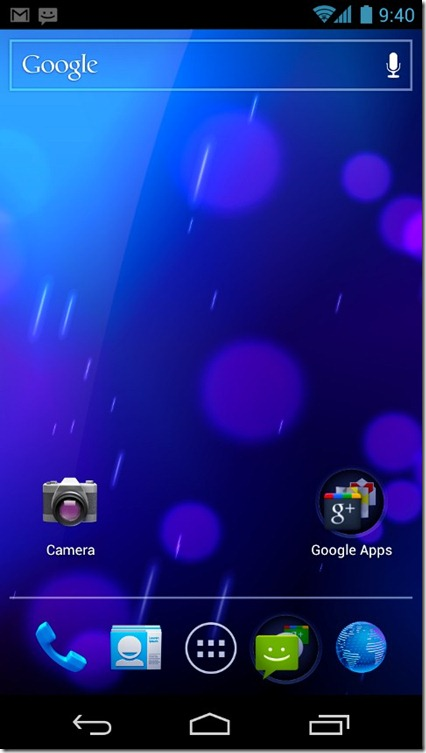
\includegraphics[height=7cm]{imagenes/capitulo2/ics-homescreen.jpg}
	}
	\hspace{0.8cm}
	\subfloat[Teclado deslizante]{
	          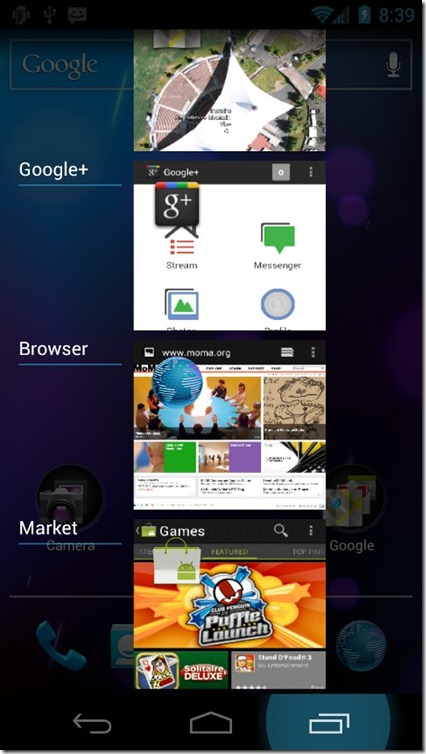
\includegraphics[height=7cm]{imagenes/capitulo2/ics-multitasking.jpg}
	}	
	\caption{Novedades de la versión Ice Cream Sandwich}
\end{figure}


\subsection{Jelly Bean}

El 9 de julio del 2012 se presenta la versión 4.1 de Android, conocida como Jelly Bean. Esta versión se caracteriza por:
\begin{itemize}
\item Mejora la interfaz, integrando el proyecto Butter, ofreciendo una sensación de fluidez mayor al manejar el dispositivo.
\item Agrega nuevas funcionalidades a la aplicación de la cámara. Las posibilidad de crear imágenes panorámicas en 360 grados es la más destacable.
\item Soporte multi-usuario.
\item Aplicación de inteligencia artificial, Google Now, la cúal responderá a algunas preguntas típicas relacionadas con el tiempo, eventos, vuelos, lugares, tráfico, resultados deportivos\ldots
\item Teclado predictivo deslizante.
\end{itemize}

\begin{figure}[!h]
	\centering	
	\subfloat[Nueva interfaz]{
	          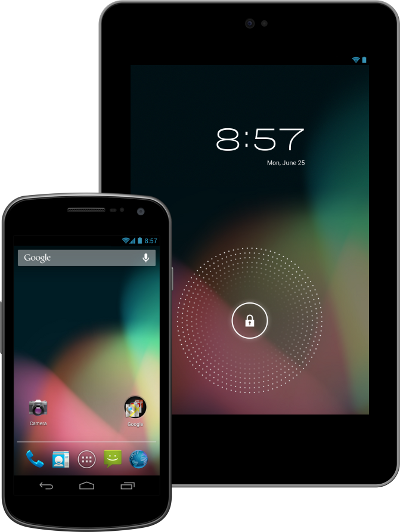
\includegraphics[height=6cm]{imagenes/capitulo2/jb-screenshot.png}
	}
	\hspace{0.8cm}
	\subfloat[Google Now]{
	          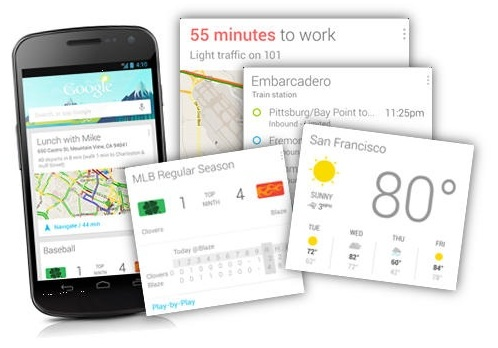
\includegraphics[height=6cm]{imagenes/capitulo2/jb-googlenow.jpg}
	}
	\caption{Novedades de la versión Jelly Bean}
\end{figure}


\subsection{Kit Kat}

Junto con el nuevo móvil de Google, el Nexus 5, el 31 de octubre de 2013 se presenta la versión 4.4 de Android, conocida como Kit Kat.  El objetivo principal de esta versión es resolver el problema de fragmetación de la plataforma, en la cual existe muchas versiones de Android. Para cubrir esta meta, se ha optimizado el uso de batería y la RAM, pudiendo ejecutarse en la mayoría de los móviles actuales.


\chapter{Computación gráfica}

El objetivo de este capítulo es explicar los conceptos técnicos necesarios parar poder comprender cómo se crean y representan animaciones en la pantalla del smartphone o cualquier otro dispositivo.
\newline

Comenzaremos explicando cúales son los datos necesarios para definir animaciones y las operaciones necesarias para poder representarlas en la pantalla, teniendo en cuenta propiedades de la luz como son la reflexión, refraccion y absorción.
\newline

Para finalizar, hablaremos de OpenGL, una librería para el tratamiento de gráficos en tres dimensiones, que será utilizada en el proyecto.  
\newpage


\section{¿Qué es la computación gráfica?}

La computación gráfica es el arte de producir imágenes con una computadora, proyectándolas sobre una superficie digital, como un televisor, un móvil  o de un cine.
\newline

La información necesaria, procesada por un algoritmo, para generar cada imagen es almacenada en un formato gráfico. Una clasificación que podemos realizar respecto a los formatos es si representan la información en dos o tres dimensiones, es decir, formatos bidimensionales o tridimensionales.
\newline 

La rasterización consiste en el algoritmo que procesa los datos almacenados en un formato gráfico, para generar una imagen, atendiendo al tamaño y  resolución correspondiente a la superficie de pantalla donde se va a visualizar.
\newline

No hemos de confundir formatos tridimensionales con las pantallas 3D. El proceso de rasterización para pantallas 3D crea imágenes manipuladas de tal forma que nuestro celebro las procesa como tridimensionales directamente o a través de algún tipo de periférico como gafas polarizadas. 

\section{Formatos bidimensionales (2D)}

Cuando hablamos de formatos bidimensionales, nos referimos directamente a las imágenes. A su vez, este formato puede ser representado de dos formas:

\begin{itemize}
\item \textbf{Mapa de bit} (jpg y bmp): La imagen es almacenada como una cuadricula, en la que se indica qué color tiene cada celda. Lo más común es representar los datos usando métodos de compresión que reducen significativamente su tamaño. La resolución\footnote{Tamaño de la imagen expresado en pixeles de alto por ancho} de la imagen esta directamente relacionada con el número de celdas capaz de representar. 
\item \textbf{Vectoriales} (ps y svg): La imagen es guardada utilizando fórmulas matemáticas básicas como son círculos, cuadrados, elipses\ldots\ por lo que no está definida su resolución. Su tamaño viene determinado por la complejidad de la imagen y no por su resolución.
\end{itemize}

\begin{figure}[h]
	\centering	
	\subfloat[Mapa de bit]{
	          
\includegraphics[height=2.5cm]{img/bitmap.jpg}
	}
	\subfloat[Vectorial]{
	          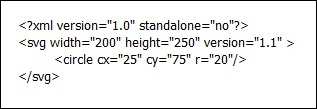
\includegraphics[height=2.5cm]{img/vectorial.jpg}
	}
	\caption{Representación de un circulo}
\end{figure}

Existe formatos tan comunes como pdf que son híbridos, es decir, algunas regiones del documento son representadas de forma vectorial y otras como mapas de bit.
\newpage

Si nos centramos en el proceso de rasterización, los formatos en mapa de bits son mucho más ligeros que los vectoriales, esto se debe a que existe una relación casi directa entre las celdas del mapa de bit y los píxeles de pantalla. 
\newline 

Sin embargo, como la resolución de una mapa de bit esta implícito en el formato, en algunos casos pueden provocarse errores en la rasterización conocidos como aliasing. Estos errores se producen cuando se adapta a la resolución de la pantalla donde se va a visualizar. Para corregir esta problemática, existen distintos tipos de filtros conocidos como \textbf{antialiasing}, los cuales son capaces de detectar aquellos píxeles conflictivos  y cambiar su color a uno más apropiado. 

	\begin{figure}[h]
	\centering	
	\subfloat[Aliasing I]{
	          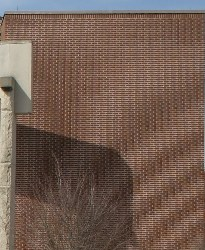
\includegraphics[width=4cm]{img/AliasedBrick0.jpg}
	}
	\subfloat[Anti-Aliasing]{
	          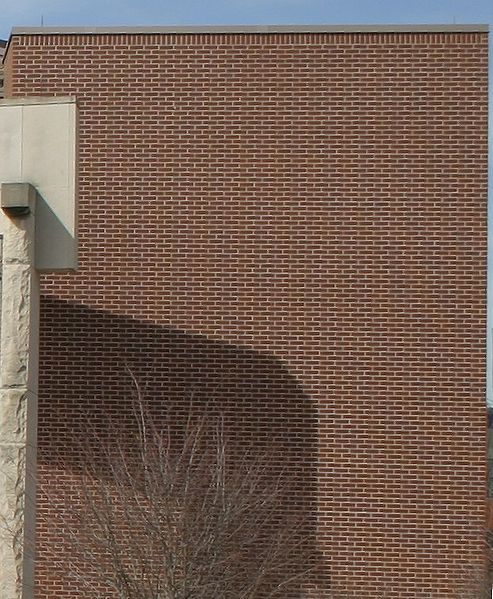
\includegraphics[width=4cm]{img/AliasedBricks1.jpg}
	}
	\caption{Efectos del aliasing y antialiasing sobre una pared de ladrillos}
	\end{figure}


La computación gráfica también abarca las animaciones o secuencias de imágenes. Como hemos visto, existe una relación directa entre un formato bidimensional y una imagen, por este motivo, para crear animaciones necesitaremos tener secuencias de formatos bidimensionales.
\newpage

	\begin{figure}[!h]
	\centering	
          
\includegraphics[height=1.5cm]{img/animacion.jpg}
	\caption{Animación de una persona corriendo}
	\end{figure}


Los videojuegos intentan crear animaciones cercanas a la realidad, proyectando los elementos en la pantalla de la forma más realista posible. Lo que implica tener en cuenta desde dónde se proyecta la imagen que estamos capturando y la iluminación existente. La única forma de poder recrear esta situación con formatos en 2D sería tener un numero infinito de imágenes, por este motivo se usan los formatos en 3D.

	\begin{figure}[h]
	\centering	
	\subfloat[Pacman (1980)]{
	          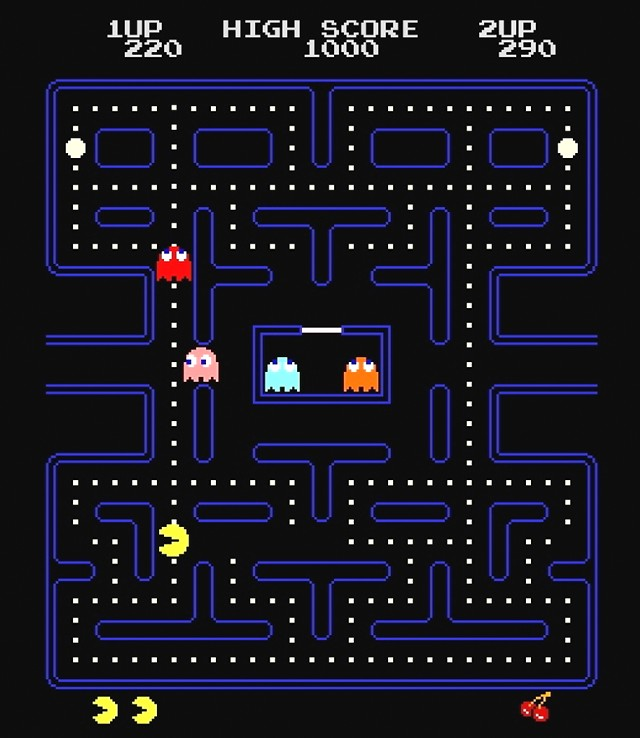
\includegraphics[height=5cm]{img/pac-man.jpg}
	}
	\subfloat[Super Mario Bros (1985)]{
	          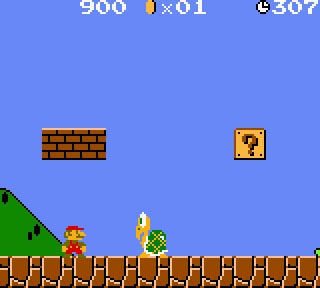
\includegraphics[height=5cm]{img/super-mario-bros.jpg}
	}

	\subfloat[Prince of persia (1989)]{
	          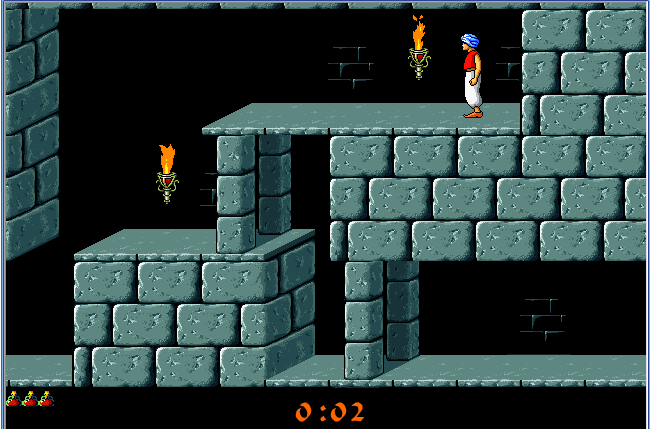
\includegraphics[width=7cm]{img/prince_of_persia.png}
	}
	\caption{Evolución de videojuegos con formato 2D}
	\end{figure}


\section{Formatos tridimensionales (3D)}

Los complejidad de los formatos 3D es muy superior comparada con los formatos 2D. Para representar una escena se ha de indicar cada uno de los elementos existentes, la iluminación y qué parte de esa escena va a ser proyectada en la pantalla. Al pensar en una escena cualquiera, por ejemplo una casa, los elementos que lo componen serían las distintas habitaciones, armarios\ldots\ La iluminación variará en función de las luces que estén encendidas y la luz que entre por las ventanas. La proyección de la escena sobre la pantalla no sólo dependerá de los elementos y la iluminación, también será influida por la posición en el que se sitúe el espectador. No vemos lo mismo si estamos sentados en el sillón o tumbados en la cama.

\subsection{Mallas}

Cada elemento de una escena es representado mediante polígonos. El conjunto de los polígonos que componen un elemento se conoce como malla o en ingles, \texttt{mesh}. En computación gráfica estos polígonos se reducen a cuadriláteros o triángulos\footnote{Actualmente los dispositivos móviles tan sólo tratan con mallas definidas por triángulos}. Cada polígono, conocido por cara o face, está formado a su vez  por tres o cuatro vértices para formar un triángulo o un cuadrado respectivamente.

\begin{figure}[h]
	\centering
	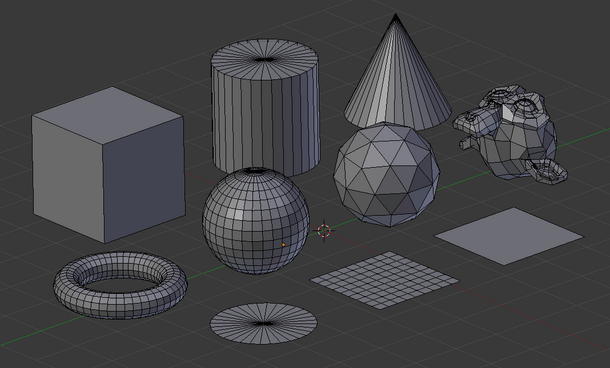
\includegraphics[width=12cm]{img/mallas.png}
	\caption{Ejemplos básicos de mallas}
\end{figure}

Ahora ya sabemos que el contorno de cada una de los elementos de la escena se realiza mediante mallas, pero desconocemos el color de la misma. Para dar color a cada una de las caras de una malla, se ha de indicar el color de cada uno de los vértices que lo componen. 


Indicar el color de los distintos vértices no es suficiente, también se han de indicar otras propiedades como son el sombreado y si aplican o no texturas, conceptos, que explicamos a continuación.

\begin{description} 

\item [Sombreado:] es un algoritmo mediante el cual se indica cómo se va a calcular el color de los píxeles intermedios dentro de cada polígono. Los principales algoritmos son:

\begin{itemize}
\item \textbf{Flat:} todos los píxeles del polígono tendrán un único color, por lo que todos los vértices también han de tener ese mismo color. Debido a su simplicidad su coste computacional es muy bajo pero los resultados son muy pixelados y por tanto de peor calidad gráfica.
\item \textbf{Gouraud:} de mayor detalle que el anterior, se centra en los vértices de cada polígono, calculando el color de cada punto de la superficie interpolando los colores de cada vértice.
\item \textbf{Phong:} es el  algoritmo más preciso para calcular el color por cada píxel, en el cual se interpolan los vectores normales de sus vértices. Por contra su coste es bastante más elevado que Gouraud. Cuando los polígonos de los elementos de la escena son más pequeños que un píxel, los algoritmos Gouraud y Phong tienen el mismo resultado.
\end{itemize}

\begin{figure}[h]
	\centering
	\subfloat[Flat]{
	          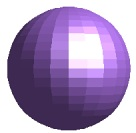
\includegraphics[height=3.3cm]{img/flat.jpg}
	}	
	\subfloat[Gouraud]{
	          \includegraphics[height=3.3cm]{img/gourad.jpg}
	}
	\subfloat[Phong]{
	          \includegraphics[height=3.3cm]{img/pong2.jpg}
	}
	\caption{Esfera con los tres tipos de sombreado}
\end{figure}


\item [Texturas:] son imágenes que se aplican sobre la malla dándole un mayor realismo. Al aplicar una textura se ha de indicar su mapeo, es decir, cómo se traslada la imagen sobre la malla. Para ello se usan las siguientes propiedades:

\begin{itemize}
\item \textbf{Repeating:} indica si la imagen se ha de repetir sobre los ejes.
\item \textbf{Clamping:} indica si se ha de extender el último píxel de la imagen sobre los ejes.

\begin{figure}[h!]
\centering	  
\includegraphics[width=12cm]{img/ClampingRepeatMapping.jpg}
\caption{Efectos de clamping y repeating}
\end{figure}

\item \textbf{UV Mapping:} indica la correspondencia entre los vértices de la malla y los píxeles de la imagen. En función de si la malla es un plano, cubo, tubo o esfera se conocen como flat, cube, tube o sphere mapping.
\begin{figure}[h]
	\centering	  
	\subfloat[Cube mapping]{
	          \includegraphics[height=2.8cm]{img/CubeMapping.jpg}
	}
	\subfloat[UV mapping]{
	          \includegraphics[height=2.8cm]{img/textura_uvMapping.jpg}
	}
	\caption{Ejemplos de mapeos}
\end{figure}
\label{funcionesMapeo}
\item \textbf{Función de mapeo:} determina cómo afecta la textura sobre el objeto. Entre las funciones más conocidas podemos destacar:


\begin{itemize}
\item \textbf{Dispacement mapping:} técnica utilizada para deformar una malla mediante una textura. Consiste en desplazar cada vértice de la malla una distancia determinada por la imagen asociada a la textura. 

\begin{figure}[h]
\centering	  
\includegraphics[height=4.5cm]{img/Displacement.jpg}
\caption{Ejemplo de displacement mapping}
\end{figure}

\item \textbf{Normal mapping:} técnica que consiste en modificar las normales\footnote{Las normales o vector normal es el vector perpendicular al plano formado por los vértices.} de una malla, aplicando un desplazamiento definido por una textura, de esta forma se consigue un mayor detalle con menos vértices. Hay que tener en cuenta que al no modificar la geometría del objeto tampoco lo harán sus sombras.\begin{figure}[ht]
\centering	  
\includegraphics[height=4cm]{img/NormalMapping.jpg}
\caption{Ejemplo de normal mapping}
\end{figure}
 

\end{itemize}
\end{itemize}

\end{description}

Otras de las ventajas que nos ofrece los modelos 3D es la posibilidad de articular las mallas mediante un nuevo concepto, la armadura. 
\newline

\label{sec:armadura}
La armadura es una especie de esqueleto, compuesto por varias articulaciones, que al moverse, se traslada dicho movimiento sobre los vértices cercanos que la componen. En las películas de animación estas armaduras son creadas a partir de unos trajes que contienen multitud de sensores, los cuales transmiten información sobre cualquier movimiento que realizan.
\begin{figure}[h]
	\centering	  
	\subfloat[Armadura]{
	          \includegraphics[height=5cm]{img/armadura1.png}
	}
	\subfloat[Pose 1]{
	          \includegraphics[height=5cm]{img/armadura2.png}
	}
	\subfloat[Pose 2]{
	          \includegraphics[height=5cm]{img/armadura3.png}
	}
	\caption{Armadura sobre un guerrero}
\end{figure}




\subsection{Cámaras}

Mediante el concepto de cámara se indica el lugar desde el cual, la escena va a ser proyectada sobre la pantalla. De cada una de las cámaras de una escena hemos de conocer su posición y orientación mediante los siguientes parámetros:
\begin{itemize}
	\item  \textbf{Eye:} define la posición de la cámara en el espacio.
         \item  \textbf{Center:} define el punto al cual estamos mirando.
         \item  \textbf{Up:} define el vector vertical a la cámara.
	\begin{figure}[!h]
		\centering
	         	 \includegraphics[width=7.5cm]{img/glulookat.jpg}
		\caption{Posición y orientación de una cámara}
	\end{figure}
\end{itemize}

También hemos de establecer los siguientes parámetros de la cámara, a través de los cuales se determinará el área visible de la escena. 
\begin{itemize}
\item  \textbf{Fovt:} define el ángulo de apertura de la cámara 
\item  \textbf{Aspect:} define la proporción entre ancho y alto de la imagen (16:9, panorámico, 4:3, etc)
\item \textbf{ Near:} define la distancia al plano de corte cercano a la cámara
\item  \textbf{Far:} define la distancia al plano de corte más alejado de la cámara.
\end{itemize}
\begin{figure}[!h]
	\centering
	          \includegraphics[width=7cm]{img/gluperspective.png}
	\caption{Frustrum de una cámara}
\end{figure}

\subsection{Luces}

En cada escena hay que indicar los distintos focos de luz existentes, por cada uno de ellos se han de especificar las siguientes propiedades:

\begin{itemize}
	\item \textbf{Color:}  de la luz que emite el foco.
	\item \textbf{Intensidad:} con la que la luz es emitida y cómo se va atenuando con la distancia.
	\item \textbf{Tipo de luz:}
	\begin{itemize}
		\item Directional light: es un tipo de luz ubicada en el infinito, por ejemplo el Sol.
		\item Point light: es un tipo de luz posicionada en un punto que emite luz en todas las direcciones, por ejemplo, una bombilla.
		\item Spot light: es un tipo de luz similar al Point Light pero sólo emite protones bajo una superficie conoidal, determinada por un vector direccional y el angulo de corte. Un ejemplo claro de este tipo de luz es un linterna.
	\end{itemize}
	
	\begin{figure}[!h]
	\centering
	\subfloat[Tipos de luces]{
	          \includegraphics[width=7cm]{img/typeoflight.jpg}
	}

	\subfloat[Iluminación aplicada a un plano]{
	          \includegraphics[width=7cm]{img/typeoflight2.jpg}
	}
	\caption{Tipos de luces y el efecto sobre un plano}
	\end{figure}
\end{itemize}


\section{Modelos de iluminación}\label{modeloIluminacion}

En puntos anteriores se han determinado distintos elementos que forman una escena, hemos identificado el color de las mallas, pero el color real en la escena depende de muchos factores. Si observamos un objeto de color blanco a plena luz del día, lo veremos blanco, pero si ese mismo objeto lo encontramos en una habitación con una luz roja, diremos que es rojo, por lo tanto, el color de los focos de luz existentes es un factor a tener en cuenta en la iluminación de una escena. También hay que tener en cuenta que la luz emitida por los focos puede estar siendo bloqueada por otras mallas de la escena, provocando sombras. Los modelos de iluminación son los responsables de determinar el color real del objeto en función de estos factores y muchos otros.
\newline

Para poder entender los modelos de iluminación se exponen a continuación una serie de conceptos de óptica básicos y cómo son trasladados a una computadora.

\subsection{Conceptos ópticos básicos}

La óptica puede ser estudiada pensando en su geométrica, física o cuántica, nos centraremos en la geométrica que es la utilizada en las computadoras para simular el comportamiento de la luz.
\newline

\begin{figure}[h]
	\centering
	          \includegraphics[width=14cm]{img/espectroElectromagnetico.png}
	\caption{Espectro electromagnético de la luz}
\end{figure}

La óptica geométrica está fundamentada en la teoría de los rayos de luz. Esta teoría considera que todo objeto visible emite rayos rectos de luz en todas direcciones a su alrededor. Cuando estos rayos inciden sobre otros cuerpos, se presentan los siguientes fenómenos ópticos:

\begin{description}
\item [Reflexión:] el rayo de luz es proyectado en sentido contrario al que incide sobre el objeto. Dependiendo del material del objeto existen dos tipos de reflexión:
\begin{itemize}
	\item \textbf{Difusa:} el rayo incidente es reflejado en un amplio abanico de direcciones con intensidades equivalentes, debido a rugosidades en el material. 
	\item \textbf{Especular:} el rayo incidente es reflejado en una única dirección y con el mismo ángulo con el que incide en el objeto.  
\end{itemize}

La reflexión lleva asociada una pérdida de intensidad lumínica en función de las características del objeto con el que haya colisionado el rayo de luz.  Cuanta más luz retenga el objeto, menor será la intensidad del rayo reflejado.

\begin{figure}[h]
	\centering
	\subfloat[Difusión]{
	          \includegraphics[width=5cm]{img/reflexion_difusa.jpg}
	}
	\subfloat[Especular]{
	          \includegraphics[width=5cm]{img/reflexion_especular.jpg}
	}
	\caption{Fenómenos de reflexiones difusa y especular}
\end{figure}
\item [Refracción:] es el cambio de dirección que experimenta un rayo de luz al pasar de un medio a otro. Este cambio de dirección es lo que provoca que veamos torcido un lápiz al ser sumergido en el agua.
\begin{figure}[h]
	\centering
	          \includegraphics[width=4cm]{img/refraction.jpg}
	\caption{Fenómeno refracción sobre el agua}
\end{figure}
\item [Absorción:] cuando un rayo luminoso se propaga, va disminuyendo paulatinamente su intensidad, siendo absorbida poco a poco por el entorno, dotándole de color.  Si un objeto absorbe todos los colores de la luz menos el verde, el ojo humano percibirá dicho objeto de color verde.
\end{description}


\subsection{Aproximación a un modelo computacional}

Hasta el momento hemos hablado del color de las luces y las mallas, lo cual es una simplificación. En un modelo computacional hemos de hablar de la cantidad de luz que absorben las mallas o emiten las luces. El espectro luminoso de la luz se representa por el modelo RGB, es decir, los niveles de rojo, verde y azul. 
\begin{figure}[h!]
	\centering	  
	\subfloat[Cubo de luz]{
	          \includegraphics[height=4cm]{img/RGBCube.jpg}
	}
	\subfloat[Colores principales]{
	          \includegraphics[height=4cm]{img/RGBCube2.jpg}
	}
	\caption{Visualización del espectro de luz sobre un cubo RGB}
\end{figure}

La luz es descompuesta en los siguientes tipos de luces:
\begin{itemize}
\item \textbf{Luz ambiental:} es aquella que proviene de una fuente que ha sido tan disipada por el entorno que es imposible determinar su dirección.
\item \textbf{Luz de difusión:} es aquella sobre la que será aplicado el fenómeno de difusión generando objetos con un contorno suavizado y pudiendo observar su forma tridimensional.
\item \textbf{Luz especular:} es aquella sobre la que será aplicado el fenómeno de reflexión especular, generando brillos en los objetos.
\item \textbf{Luz de emisión:} se corresponde con la luz que emite un objeto. Por motivos de simplificación, suele tratarse como un incremento de la luz ambiental específica para dicho objeto.
\end{itemize}

Aplicando este modelo a una luz en nuestro escenario, hemos de establecer el nivel de luz ambiental, de difusión y especular sobre cada uno de los focos de luz y sobre cada objeto. Además deberemos saber cúal será su comportamiento ante el fenómeno de absorción de la luz, es decir, cuáles son los niveles de luz ambiental, difusión y especular que absorberá, además de la luz de que emite el objeto por si mismo. 

\subsection{Clasificación de modelos de iluminación}

Ahora que conocemos las propiedades ópticas básicas, podemos centrarnos en el concepto de modelo de iluminación, a través del cual, se va a determinar cómo se va a simular en la computadora el comportamiento de la luz sobre los objetos. 
\newline 

Los modelos se clasifican principalmente por el tipo de iluminación. En el modelo de \textbf{iluminación directa} únicamente están implicados los rayos de luz procedentes de una fuente de luz y que colisionan con un objeto. Ahora sabemos que este rayo de luz puede sufrir el fenómeno de reflexión, modificando las propiedades del rayo, el cual puede volver a colisionar con otros objetos. Los rayos procedentes de la reflexión son descartados en modelos de iluminación directa, pero en los que se fundamentan los modelos de \textbf{iluminación global}.
\newline

Los métodos de iluminación global generan escenas difícilmente distinguible de la realidad, es lo que se conoce como foto-realismo pero no son aplicables al mundo de los videojuegos debido a su elevado coste computacional. Están surgiendo nuevos modelos de iluminación híbridos, dando origen al término de  foto-realismo animado. 

\begin{figure}[h]
	\centering
	          \includegraphics[width=11cm]{img/fotorealismo.jpg}
	\caption{Imágenes del juego Crysis 2 comparadas con la realidad}
\end{figure}

A continuación se muestra un listado de modelos de iluminación más populares, entre los cuales nos centraremos en Phong y Radiosity:

\begin{itemize}
\item \textbf{Lambert:} modelo de iluminación directa, ideal para superficies plásticas ya que esta basado en superficies difusas perfectas, por lo tanto, sobre el modelo de reflexión especular.
\item \textbf{Oren-Nayar:} modelo de iluminación directa, ideal para superficies fibrosa como ropa, madera y pelo. Está basado en superficies difusas borrosas, es decir, un modelo de reflexión de difusión.
\item \textbf{Phong:} modelo de iluminación directa basado en superficies especulares, ideal para elementos con superficies parecidas a un espejo sin llegar a serlo, como pinturas con brillo y metales.
\item \textbf{Radiosity:} modelo de iluminación global basado en el nivel de calor absorbido por los elementos puramente difusos.
\item \textbf{Ray-tracing:} modelo de iluminación global que simula el trazado de rayos de luz desde el observador. Por cada uno de los rayos simulados se tiene en cuenta los fenómenos de reflexión y refracción.
\end{itemize}

\subsection{Modelo de iluminación de Phong}

Es un modelo de iluminación directa, desarrollado en 1973 por Bui Tuong Phong en la universidad de Utah, basándose en la combinación de reflexión especular y difusión, nivel de brillo de la superficies, iluminación ambiental y atenuación de la luz. 
\newline 

En el modelo de iluminación de Phong, el color en un punto $P$ en una superficie cuyo material está definido por $K$, donde 
      $$ K = \{ K_{ambiental}, K_{difusión}, K_{especular} \}$$ 
Y sobre el que se aplica una luz con una intensidad definida por $ L $ donde 
$$ L = \{ L_{ambiental}, L_{difusión}, L_{especular}\} $$ 
Se determina por la suma de las intensidades de luz reflejadas, es decir: 
$$ Color = Color_{ambiental} + Color_{diffusión} + Color_{especular} $$ 

\begin{figure}[h]
	\centering
	          \includegraphics[width=11cm]{img/PhongComponent.png}
	\caption{Modelo de iluminación de Phong}
\end{figure}


Para el calculo del color final del objeto se tendrán en cuenta los vectores formados por la posición de la luz, el observador y el punto de colisión entre el rayo de luz y el objeto, a este punto lo llamaremos $P$. A partir de estos tres puntos se han de calcular:
\begin{itemize}
\item El vector normal de la superficie en $ P $ se define como $  \vec{n} $.
\item El vector entre el punto donde se ubica la cámara y el punto $P$ se define como   $ \vec{v}$.
\item El vector entre el origen de la luz y el punto $ P $ se define como  $  \vec{l} $ y forma un angulo $\theta$ con respecto a la normal.
\item El vector de la luz reflejado en el mismo angulo $\theta$ respecto a la normal se define como $ \vec{r}$.
\end{itemize}

\begin{figure}[h!]
	\centering
	          \includegraphics[width=7cm]{img/phongVector.jpg}
	\caption{Vectores utilizados en el modelo Phong}
\end{figure}

\begin{description}
\item [El componente ambiental] se corresponde con el producto de la intensidad de la luz ambiental sobre los materiales de emisión y ambiental, es decir: 
	$$ Color_{ambiental} = ( K_{ambiental} + K_{emision} ) * L_{ambiental} $$

\item [El componente de difusión] se calcula con la intensidad de la luz de difusión, aplicada al material correspondiente, pero teniendo en cuenta el ángulo existente entre la normal y el vector de la luz. Cuanto más pequeño sea el ángulo entre los vectores, mayor será su producto escalar, por lo que recibirá más luz. Si el punto de luz está muy alejado, el producto vectorial puede resultar negativo, por lo que no llegará luz y el valor se redondeará a cero. 
	$$ Color_{difusión} = K_{difusión} * L_{difusión} *max(\vec{n} \cdot \vec{l}, 0)$$

\item [El componente especular] depende del punto de vista del observador sobre el rayo reflejado. El producto escalar entre ambos vectores es tratado de igual forma que en el componente de difusión.
	$$ Color_{especular} = K_{especular} * L_{especular} *max( \vec{r} \cdot \vec{v}, 0)$$

\end{description}

\subsection{Modelo de iluminación por radiosidad}

La radiosidad se fundamenta en el estudio térmico de la luz debido a la vibración de los fotones, determinando que una superficie estará más iluminada cuanto más fotones choquen contra ella o lo que es lo mismo, tenga un mayor nivel de radiosidad. 
\newline 

Nos encontramos con un modelo de iluminación global y con un comportamiento de los objetos puramente difuso. Todos los rayos de luz son reflejados de forma homogénea y con la misma intensidad en todas direcciones, restándole parte de su calor o intensidad limúnica inicial, debido al fenómeno de absorción.
\newline 

\begin{figure}[h!]
	\centering
	          \includegraphics[width=7cm]{img/radiositymodel.jpg}
	\caption{Modelo de radiosidad donde podemos observar en rojo una luz directa que es reflejada y sus rayos indirectos que se muestran en verde}
\end{figure}

La radiosidad en un determinado punto, $ B_i $ se define cómo la energía por unidad de área que emite una superficie por unidad de tiempo, que no es más que la suma de la luz emitida por la superficie y la energía reflejada proveniente de otras superficies:
	$$ B_I = E_i + R_i \sum B_jF_{ij} $$ 
Donde:
\begin{itemize}
\item $E_i$: energía emitida por la superficie $i$.
\item $R_i$: capacidad de reflexión de la superficie $i$.
\item $B_j$: energía transmitida de la superficie $j$ sobre $i$.
\item $F_{ji}$: factor de forma entre $i$ y $j$ que mide la cantidad de energía que emitida por $j$ llega a $i$.
\end{itemize}

Finalmente, en cada punto de la escena, se calcularán los componentes ambiental, especular y de difusión del escenario, basándose en la intensidad de luz, calculada previamente en el modelo de radiosidad.
\newline

\begin{figure}[h!]
	\centering
	          \includegraphics[width=10cm]{img/radiosity_comparison.jpg}
	\caption{Comparativa de una escena procesada con radiosidad y phong}
\end{figure}

Las ventajas y desventajas de este modelo de iluminación son las siguientes:
\begin{itemize}
\item La calidad de la imagen es cercana a la realidad.
\item El tiempo de procesamiento es elevado.
\item Se puede generar un procesamiento progresivo, es decir, en cada paso se puede ver la escena, incrementando su realismo cuantos más pasos se realicen. Cada paso  consiste en calcular los nuevos rayos generados por la reflexión.
\item La radiosidad de la escena no cambia ante cambios de cámara por lo que no ha de ser recalculada por los movimientos de la cámara.
\item La radiosidad de la escena cambia al cambiar la posición de cualquier elemento de la escena, pudiendo cambiar la trayectoria de algunas rayos y por lo tanto, la radiosaidad de las superficies. Este es el motivo por el cual no resulta útil en el desarrollo de videojuegos.
\item Para calcular la radiosidad de la escena no se usan los polígonos que componen las distintas mallas debido a su elevado número, para acelerar este cálculo se utilizan unas superficies más amplias. Debido a esta simplificación se pueden ocasionar algunos errores en el calculo de la radiosidad.
\end{itemize}

\section{Librerías de computación gráfica}

Debido a la complejidad de las escenas en tres dimensiones, surgen unas librerías de uso común para simplificar estas tareas al desarrollar aplicaciones. Las librerías más conocidas en el mercado son:
\begin{itemize}
\item La desarrolla por Microsoft, \textbf{DirectX}, que está limitada para entornos con un sistema operativo Windows.
\item Las basadas en el API de \textbf{OpenGL}, implementadas para sistemas operativos Unix, Linux, Windows, etc.
\end{itemize}
\begin{figure}[h!]
	\centering	  
	\subfloat[DirectX]{
	          \includegraphics[height=2.5cm]{img/DirectX-Logo.jpg}
	}
	 \hspace*{1cm}
	\subfloat[OpenGL]{
	          \includegraphics[height=2.5cm]{img/OpenGL_logo.png}
	}
	\caption{Logotipos de las librerías}
\end{figure}

DirectX no está soportada en Android, por lo que nos centraremos en OpenGL, para ser más exactos, sobre \textbf{OpenGL ES}, una versión más optimizada para los sistemas con un bajo nivel de procesamiento. En esta versión se han simplificado sus operaciones pero sin alterar su funcionalidad. Existen tres versiones:
\begin{description}
\item [OpenGL ES 1.0:] procede de OpenGL 1.3 e implementa un modelo de iluminación de Phong en el pipeline fijo del microprocesador de la tarjeta gráfica.
\item [OpenGL ES 1.1:] es una evolución de la 1.0 añadiendo ciertas mejoras de OpenGL 1.5. 
\item [OpenGL ES 2.0:] procede de OpenGL 2.0, que da un gran salto al incluir un pipeline dinámico, al que poder incorporar en algunos de sus pasos los shaders, a partir de los cuales se puede crear un modelo de iluminación acorde a las necesidades de cada proyecto.
\end{description}

 Los shaders son códigos fuente compilados e interpretados por los microprocesadores de las tarjetas gráficas en tiempo de ejecución. Están escritos en un nuevo lenguaje llamado GLSL (Graphics Library Shaders Languaje). Para entender cómo funcionan hemos de conocer la estructura de OpenGL 2.0.

\subsection{OpenGL 2.0}

Toda tarjeta gráfica que soporte OpenGL 2.0 estará compuesta por un pipeline con una estructura similar al mostrado en el siguiente gráfico. Se han identificado con cajas sombreadas aquellas fases en las que es posible insertar shaders.
\newline

\begin{figure}[h!]
\centering
\includegraphics[width=11.5cm]{img/OpenGL_Pipeline2.jpg}
\caption{Pipeline en OpenGL ES 2.0}
\end{figure}

La primera fase \texttt{Vertex Array/Buffer Object} se corresponde a la adaptación de los datos definidos en el API a la estructura hardware dependiente de la tarjeta, por este motivo no haremos hincapié en ella.

\subsubsection{Vertex Shader}

En esta segunda fase se realizan operaciones sobre los vértices de cada malla, de uno en uno, por lo que se desconoce la forma de la malla. Las operaciones más frecuentes son transformaciones afines, proyecciones, transformaciones de color, coordenadas de textura e iluminación. La entrada de esta fase está constituida por:
\begin{itemize}
\item \textbf{Atributos:} propiedades inherentes a los vértices (coordenadas de textura, vector normal\ldots) que pueden ser definidas o creadas por la aplicación de OpenGL para cada vértice. 
\item \textbf{Uniforms:} propiedades generales a todos los vértices que pueden ser definidas por la aplicación de OpenGL como una constante.
\item \textbf{Samplers:} se corresponden con las texturas, siendo opcionales en esta fase.
\end{itemize}

Es obligatorio definir el \textbf{GL\_Position}, que se corresponde con la posición final del vértice. Las variables GL\_PointSize y GL\_FrontFacing son opcionales. Indican el tamaño en píxeles del vértice y la ecuación del plano de corte respectivamente. Para comunicarse con otras fases del pipeline se utilizan variables de tipo varying.
\newline

A modo de ejemplo, a partir de un vertex shaders, podríamos ser capaces de modificar los vértices de una malla junto con una textura, aplicando la técnica de dispacement mapping, descrita en la página 39, cuando se definía el concepto de malla.

\begin{figure}[H]
\centering
\includegraphics[width=11cm]{img/VertexShader.jpg}
\caption{OpenGL ES 2.0 Vertex Shaders}
\end{figure}

\subsubsection{Primitive Asemmbly y rasterización}

La tercera fase consisten en agrupar los vértices formando puntos, lineas o polígonos para después ejecutar la rasterización y obtener los fragmentos que van a componer la imagen. 

\begin{figure}[!h]
\centering
\includegraphics[width=4.5cm]{img/rasterization.png}
\caption{Ejemplo de rasterización}
\end{figure}

\subsubsection{Fragment Shader}

En la cuarta fase, programable mediante un shader, recibe los fragmentos obtenidos en la fase anterior. Sobre estos segmentos se pueden aplicar operaciones de mapeo de texturas, mezcla de colores, efecto de niebla\ldots
\newline

El objetivo del fragment shaders es conseguir el color del fragmento, almacenado en la variable \textbf{GL\_FragColor}, utilizando un modelo de iluminación con los siguientes datos y las variables de tipo uniform y varying, definidas previamente:
\begin{itemize}
\item \textbf{GL\_FragCoord:} indica las coordenadas del fragmento.
\item \textbf{GL\_FontFacing:} indica si el fragmento está oculto por otro fragmento.
\item \textbf{ GL\_PointCoord:} coordenadas de dispersión aplicado sobre las partículas\footnote{El concepto de partículas esta fuera del alcance del proyecto y es usado para simular objetos muy dinámicos como son fuegos artificiales.}.
\end{itemize}

\begin{figure}[H]
\centering
\includegraphics[width=11.5cm]{img/FragmentShader.jpg}
\caption{OpenGL ES 2.0 Fragmen Shaders}
\end{figure}

Algunas de las características que pueden ser implementadas en el fragment shader son la aplicación de mapeos usando texturas, simulación de efectos de niebla, etc.

\subsubsection{Per-Fragment}

En esta última fase se genera el buffer final, equivalente a los píxeles de la pantalla. Sobre cada uno de los fragmentos se ejecutan los siguientes test, aunque inicialmente están todos deshabilitados:
\begin{itemize}
\item \textbf{Scissor box testing:} elimina todos los píxeles fuera del área de visualización, el cual se determina con las propiedades de la cámara.
\item \textbf{Stencil buffer testing:} genera una máscara de la imagen a partir de una función \texttt{glStencilFunc}. La aplicación más conocida de este stencil buffer consiste en la generación de sombras.
\item \textbf{Depth buffer testing:} elimina todos aquellos fragmentos que no están visibles al ser ocultados por otros.
\item \textbf{Blending:} fusiona el color de los segmentos que se solapen en pantalla. A través de esta técnica se puede generar el efecto de transparencia de elementos como el cristal.
\item \textbf{Dithering:} ajusta los colores disponibles que no se adaptan a los colores que han sido calculados con él modelo de iluminación. Éste tipo de técnica consiste en intercalar los píxeles para que visualmente ofrezca un color similar al que deseamos.
\end{itemize}


\begin{figure}[H]
\centering
\includegraphics[width=11.5cm]{img/dithering.jpg}
\caption{Ejemplo de dithering sobre escala de grises}
\end{figure}

\chapter{Leyes físicas en computadoras}

En este capítulo se explicará la relación existente entre la física y los videojuegos. Las dos líneas a tratar serán:
\begin{itemize}
\item Conocer la nueva posición de un objeto en movimiento transcurrido un tiempo determinado.
\item Saber cómo detectar cuando dos objetos han colisionado.
\end{itemize}

Estos conocimientos son necesarios para poder comprender las decisiones de diseño tomadas en la implementación del TfcGameEngine.

\newpage

%%%%%%%%%%%%%%%%%%%%%
%%%         INTRODUCCION              %%%
%%%%%%%%%%%%%%%%%%%%%

\section{Aplicación de la física en un videojuego}

A la hora de desarrollar un videojuego, nos encontraremos con la necesidad de simular el comportamiento de un mundo real. Esto implica incluir los efectos físicos existentes en nuestro entorno como son la velocidad, aceleración, gravedad\ldots
\newline 

Desde el punto de vista de desarrollo de un videojuego nos podríamos preguntar lo siguiente:
\begin{itemize}
\item ¿Cuál será la posición de un elemento, trascurridos 3 segundos, que viaja a una velocidad y dirección determinada?
\item ¿Cómo sabemos si dos objetos han chocado?
\item ¿Qué ocurre cuando choca una bola de billar contra otra en un determinado ángulo y fuerza?
\item ¿Cómo se mueve el líquido de un vaso situado en un objeto que está acelerando? 
\end{itemize}

En una computadora no existen leyes físicas, por lo tanto, han de ser recreados matemáticamente simulando las leyes físicas. De no ser así, podrían ocurrir cosas extrañas en la realidad, como que dos objetos ocuparan el mismo espacio.
\newline

En las siguientes secciones, para poder responder a las preguntas formuladas, se va a realizar un acercamiento sobre el origen del movimiento y para finalizar se estudiará el cálculo de las colisiones entre objetos.

%%%%%%%%%%%%%%%%%%%%%
%%%       MECÁNICA FÍSICA            %%%
%%%%%%%%%%%%%%%%%%%%%

\section{Origen del movimiento}

El movimiento es un fenómeno físico, el cual se puede definir como cualquier cambio de posición, en el espacio, que experimentan los cuerpos de un sistema con respecto a ellos mismos o a otro cuerpo, que se toma como referencia, definiendo una trayectoria.
\newline

En física, la rama que estudia y analiza el movimiento de los cuerpos es la mecánica, la cual se divide en 4 grandes ramas:
\begin{itemize}
\item Mecánica clásica (no relativista)
\item Mecánica clásica relativista
\item Mecánica cuántica 
\item Mecánica cuántica de campos
\end{itemize}

Pondremos nuestra atención sobre la mecánica clásica, la cual se ajusta más al mundo físico de un videojuego, el resto de ramas se centran en el estudio del movimiento a nivel atómico o de objetos cercanos a la velocidad de la luz.
\newline

Un subconjunto de la mecánica clásica es la física Newtoniana, que nos permite realizar un estudio de objetos sólido-rígidos, es decir, objetos que no se pueden deformar, por otro lado, la física de medios continuos nos permite el estudio de los objetos son fluidos o sólidos deformables.
\newline

En del ámbito del proyecto nos centraremos en la física de objetos sólidos, aunque en los juegos de última generación incluyen física de fluidos y objetos deformables. Debido a la complejidad de éste tipo de cálculo y con el objetivo de optimizar al máximo los recursos, existen implementaciones directamente en el hardware de las tarjetas gráficas, como es el caso de PhysX de la compañia Nvidia. 
\newline

El siguiente diagrama muestra un árbol con las distintas ramas en las que se divide la física mecánica. En color verde y naranja se han identificado las ramas que han sido aplicadas totalmente o parcialmente en el proyecto, sobre las cuales se profundizará en las siguientes secciones. En color amarillo se indican aquellas ramas que ya forman parte de los motores de juegos profesionales.

\begin{figure}[h]
	\centering	
         \includegraphics[width=12cm]{img/FisicaMecanica.jpg}
	\caption{Disciplinas de la física mecánica}
\end{figure}


\subsection{Cinemática} 

La cinemática se centra en las trayectorias de los objetos sin tener en cuenta las causas que producen el movimiento. Utiliza un sistema de coordenadas para describir las trayectorias, denominado sistema de referencia. La velocidad y la aceleración son las dos principales cantidades que describen cómo cambia su posición en función del tiempo.

\begin{itemize} 
\item \textbf{Posición ($\vec{x}$): } situación del objeto respecto al sistema de referencia.
\item \textbf{Velocidad ($\vec{v}$):}  ritmo con que cambia la posición un cuerpo.
\item \textbf{Aceleración ($\vec{a}$):} La aceleración es el ritmo con que cambia su velocidad
\item \textbf{Tiempo (t)} 
\end{itemize}

A continuación se muestran las trayectorias típicas en la cinemática y cómo se calcula la posición final '$x$' trascurrido un tiempo '$t$'.

\begin{description}
\item [Movimiento rectilíneo uniforme:] describe una trayectoria recta a una velocidad constante '$v$', sin aceleración y desde una posición inicial $\vec{x_0}$.
$$ \vec{x} = \vec{x_0} + \vec{v}t $$

\begin{figure}[!h]
	\centering	
         \includegraphics[height=3.7cm]{img/Cinematica_MRU.png}
	\caption{Evolución del movimiento respecto al tiempo}
\end{figure}

\item [Movimiento rectilíneo uniformemente acelerado:] describe una trayectoria recta desde un punto $\vec{x_0}$, una velocidad inicial $\vec{v}$ y una aceleración constante $\vec{a}$.

$$ \vec{x} = \vec{x_0} + \vec{v} t + \frac{1}{2} \vec{a}  t^2 $$

\begin{figure}[!h]
	\centering	
        \includegraphics[height=8cm]{img/Cinematica_MRUA.png}
	\caption{Evolución del movimiento respecto al tiempo}
\end{figure}

\item [Movimiento parabólico:]  es la unión de un avance horizontal rectilíneo uniforme y un lanzamiento vertical hacia arriba, que es un movimiento rectilíneo uniformemente acelerado hacia abajo por la acción de la gravedad. Este movimiento parte de una posición inicial definida por '$x$' e '$y$' y un ángulo $\theta$.

\parbox{7cm} {
$$    x = v_{inicial} * \cos{ \theta } * t  $$
$$    y = v_{inicial} * \sin{ \theta } * t  + 1/2 a t^2  $$
}
\parbox{5cm}{\includegraphics[width=5cm]{img/cinematica_MP.png}}

\end{description}

Existe otros tipos de movimientos como son los circulares, helicoidales y armónicos simples (muelles), pero están fuera del alcance del proyecto.

\subsection{Dinámica}

La dinámica se fundamenta en el estudio de las fuerzas que se aplican sobre objetos, siendo una fuerza un cambio de aceleración. Las leyes de Newton que fundamentan esta parte de la física son las siguientes:
\begin{itemize}
\item Todo cuerpo permanece en su estado de reposo o de movimiento rectilíneo uniforme a menos que otros cuerpos actúen sobre él.
\item $\vec{F} = m \vec{a} $ La fuerza que actúa sobre un cuerpo es directamente proporcional a producto de su masa y aceleración.
\item Cuando un cuerpo ejerce una fuerza sobre otro, éste ejerce sobre el primero una fuerza igual y de sentido opuesto.
\end{itemize}

El objetivo principal que buscamos en la dinámica es conocer la implicación que tiene un choque entre dos objetos. Como podemos observar, por la segunda ley de Newton, debemos conocer el tiempo que es aplicada una fuerza sobre un objeto, para poder obtener su aceleración y con ella, aplicar los conocimientos vistos en el apartado de cinemática. Conocer el tiempo que se está aplicando una fuerza sobre un objeto implica conocer la duración de un impacto, lo cual es sumamente complejo, es por ello que surge el concepto de momento.
\newline

El momento es la magnitud física, de tipo vectorial, que mide la capacidad de ejercer una fuerza de un objeto sobre otro en función de su movimiento.
\newline

El momento lineal obedece a una ley de conservación, lo cual significa que en todo sistema cerrado (o sea uno que no es afectado por fuerzas exteriores, y cuyas fuerzas internas no son disipadoras) no puede ser cambiada y permanece constante en el tiempo.
\newline

En el mundo de los videojuegos existe un alto interés en el choque de dos objetos y la repercusión en la trayectoria del objeto. Además puede que los objetos estén conectados por una visagra o cualquier otro tipo de unión, llamada junta, implicando restricciones de movimiento, que se sumarían a las implicaciones en el movimiento de los objetos.
\newline

\begin{figure}[h]
	\centering	
	\includegraphics[width=12cm]{img/Joints.jpg}
	\caption{Ejemplos de tipos de juntas}
\end{figure}

\subsubsection{Cálculo de un choque plástico}
Aunque el juego a desarrollar en el proyecto no ha de calcular las implicaciones del choque entre dos elementos, se considera de especial interés el cálculo de choques plásticos, lo que permitirían desarrollar juegos tan famosos como Angry Birds.
\newline

En un choque plástico, los objetos involucrados no se deforman, de lo contrario, seria un choque elástico. La deformación de un objeto implicaría cálculos adicionales debido a una absorción del impacto por la estructura del objeto, implicando un cambio del momento lineal.
\newline

Dados dos objetos $o_1$ y $o_2$ plásticos que se mueven a velocidades $\vec{v_1}$ y $\vec{v_2}$ y con masas $m_1$ y $m_2$ respectivamente, como resulado de la ley de conservación del momento lineal tenemos que:

$$ m_1 \vec{v_1} + m_2 \vec{v_2} = \vec{v} ( m_1 + m_2 ) $$
Por lo que la variación de velocidad $\vec{v}$ debido al choque será:
$$  \vec{v} = \frac{ m_1 \vec{v_1} + m_2 \vec{v_2}}{ m_1 + m_2 } =$$

Aplicando la variación de velocidad a ambos objetos, las velocidades finales $\vec{v_{1_{final}}}$ y $\vec{v_{2_{final}}}$ se corresponderán con las siguientes fórmulas:
$$ \vec{v_{1_{final}}} = \vec{v_1} + \vec{v} $$
$$ \vec{v_{2_{final}}} = \vec{v_2} + \vec{v} $$
	
\begin{figure}[!h]
	\centering	
	\subfloat[Juego de billar]{
		\includegraphics[height=3cm]{img/billar.jpg}
	}
	 \hspace*{1cm}
	\subfloat[Angry Birds]{
		\includegraphics[height=3.2cm]{img/angrybirds.jpg}
	}
	\caption{Ejemplos de choque plástico}
\end{figure}
%%%%%%%%%%%%%%%%%%%%%
%%%  DETECCIÓN DE COLISIONES   %%%
%%%%%%%%%%%%%%%%%%%%%

\section{Detección de colisiones}

Ya podemos calcular la posición de los objetos según transcurre el tiempo, creando en el videojuego la ilusión de movimiento. Este desplazamiento puede provocar que dos objetos choquen entre sí debido a la composición atómica de los elementos. La física atómica impide que ambos objetos ocupen el mismo espacio, pero en los videojuegos no existen estas restricciones atómicas, por lo que han de ser calculadas matemáticamente.
\newline

En un juego en dos dimensiones el calculo de colisiones consiste en detectar si un píxel está siendo ocupado por dos elementos. Cuando usamos tres dimensiones el cálculo de colisiones se complica. Lo primero que se ha de tener en cuenta es la forma del objeto, definida mediante una malla y que en la terminología asociada a las colisiones, se define como la \textbf{forma explícita} del objeto. 
\newline

Debido a la complejidad inherente de las mallas surge un problema de eficiencia en el cálculo de colisiones, por ese motivo, las mallas de los elementos son simplificadas, creando lo que se define como la \textbf{forma implícita} del objeto.

\subsection{Forma implícita de un objeto}

La forma implícita está compuesta por figuras básicas que permiten simplificar los cálculos para detectar las colisiones. Dependiendo de cómo se ajuste la forma implícita a la explícita, el cálculo de colisiones será más preciso, pero posiblemente más costoso.
\newline

Las figuras básicas se componen la forma implícita, llamadas \textbf{superficies de contorno} \texttt(Bounding Volumenes), son volúmenes geométricos cuyo tamaño requerido para ser representados en memoria es mínimo y es fácil verificar si existe o no colisión entre ellos. A continuación se muestran las superficies de contorno más comunes.

\begin{figure}[h]
	\centering	
         \includegraphics[height=3.8cm]{img/BoundingVolumes.jpg}
	\caption{Volúmenes de contorno: Esferas, AABB (axis-aligned bounding box):  cajas alineadas con los ejes y OBB (oriented bounding box): cajas orientadas respecto a los ejes.}
\end{figure}

En un videojuego, los objetos no son estáticos, sobre ellos se pueden aplicar distintas transformaciones como traslaciones, rotaciones o movimientos derivados de una armadura\footnote{El concepto de armadura se definió en el capítulo 3 sobre computación gráfica.}. Todos estos cambios implican volver a calcular las forma implícita del objeto. A continuación se puede ver cómo afectaría una rotación sobre un avión cuyas formas implícitas se han generado con esferas o AABB.
\newline

\begin{figure}[!h]
	\centering	
         \includegraphics[width=12.5cm]{img/volumenesRotacion.jpg}
	\caption{Formas implícitas transformadasd tras una rotación}
\end{figure}

Aunque estén fuera del alcance dle proyecto, hay que mencionar la existencia de distintos algoritmos mediante los cuales es posible convertir mallas en formas implícitas. El siguiente gráfico muestra un ejemplo del resultado obtenido al aplicar uno de ellos.
\newline

\begin{figure}[h]
	\centering	
         \includegraphics[width=10cm]{img/BoundingVolumesSphereBunny.jpg}
	\caption{Simplificación de una malla de un conejo mediante esferas}
\end{figure}


\subsection{Fases en la detección de colisiones}

A pesar de esta simplificación, un objeto puede colisionar con cualquier otro de la escena, por lo tanto, el cálculo de colisiones para una escena con $n$ objetos requeriría comprobar $(n-1)+(n-2)+\ldots+1 = \frac{n(n-1)}{2}$ posibles colisiones, es decir, existe una complejidad de $O(n^2)$. 
\newline

Para simplificar esta situación el cálculo de colisiones se divide en en dos fases:
\begin{description}
\item [Broad phase:] es la fase preliminar en la que se crea una división espacial de la escena en áreas que permitan descartar colisiones entre objetos de la escena rápidamente. Las técnicas de división más habituales son:
\begin{itemize}
\item \texttt{BSP} (Binary Space Partitioning): se divide la escena recursivamente en dos particiones, generando un árbol binario, donde cada nodo está compuesto por dos hijos. 
\end{itemize}

Un objeto podría ubicarse entre dos particiones, como es el caso del objeto $E$ del gráfico. En vez de modificar la forma de la partición, se indica que el objeto esté en ambos nodos.
\begin{figure}[!h]
	\centering	
        \includegraphics[height=4cm]{img/bsp.png}
	\caption{BSP}
\end{figure}


\begin{itemize}
\item \texttt{QuadTree:} es un árbol similar al BSP donde cada nodo contiene cuatro hijos en vez de dos.
\begin{figure}[!h]
	\centering	
        \includegraphics[height=4cm]{img/quadtreecolour1.png}
	\caption{QuadTree}
\end{figure}

\item \texttt{OcTree:} es un árbol donde cada nodo contiene 8 hijos.
\begin{figure}[!h]
	\centering	
	\includegraphics[height=4cm]{img/octree.png}
	\caption{OcTree}
\end{figure}
\end{itemize}


\item [Narrow phase:] en esta segunda fase se determina si dos objetos, que están ubicados en la misma partición, están colisionando. Se aplicará un test de colisión que dependerá de la superficie de contorno elegida para crear las formas implícitas de los objetos. En la siguientes secciones se detallarán cómo se detecta si existe o no colisión para esferas y AABB.
\end{description}

\subsection{Colisiones entre esferas}

Una esfera es un cuerpo geométrico, limitado por una superficie curva cerrada, cuyos puntos equidistan de otro interior llamado centro de la esfera. Para representarla, tan sólo necesitamos en  punto $\vec{c}$ que representa el centro y la distancia $r$ de la que equidistan los puntos que definen la superficie.
\newline 

\begin{figure}[h]
	\centering	
         \includegraphics[width=3.5cm]{img/esfera.png}
	\caption{Representación de una esfera}
\end{figure}

Para determinar si dos esferas colisionan tan sólo hemos de verificar, como se indica a continuación, que la distancia entre sus centros es menor que la suma de sus radios.
\newline

Dadas dos esferas, $e_1$ y $e_2$ con radios $\vec{r_1}$ y $\vec{r_2}$ y centros $\vec{c_1}$ y $\vec{c_2}$ respectivamente, están colisionarán si:
$$ distancia ( e_1, e_2 ) > r_1 + r_2 $$

$$ distancia ( e_1, e_2 ) =  \sqrt{ (c_{1_x} - c_{2_x} )^2  + (c_{1_y} - c_{2_y})^2  + (c_{1_z} - c_{2_z} )^2  } $$

\begin{figure}[h]
	\centering	
         \includegraphics[width=4cm]{img/SphereSphereCollision.jpg}
	\caption{Colisión de esferas}
\end{figure}

\subsection{Colisiones AABB}

Las \concept{AABB}{Axis-aligned bounding box} son cajas alineadas con los ejes. Debido a ésta característica es posible definir su geometría definiendo únicamente dos puntos $\vec{p_{max}}$ y $\vec{p_{min}}$ donde: 

\parbox{7cm} {
$$ \vec{p_{max}} = \{x_{max}, y_{max}, z_{max}\} $$
$$ \vec{p_{min}} = \{x_{min}, y_{min}, z_{min}\} $$
}
\parbox{6cm}{\includegraphics[width=6cm]{img/aabb.jpg}}
\newline

Para comprobar si dos objetos $a$ y $b$, con formas implícitas de tipo AABB, colisionarán hay que verificar que no se dan estas condiciones: 
\begin{enumerate}
\item $a_{max_x} < b_{min_x}$ o $a_{min_x}> b_{max_x}$ 
\item $a_{max_y} < b_{min_y}$ o $a_{min_y}> b_{max_y}$ 
\item $a_{max_z} < b_{min_z}$ o $a_{min_z}> b_{max_z}$ 
\end{enumerate}

\subsection{Errores en el cálculo de colisiones}

Una vez implementado un detector de colisiones es posible que nos encontremos con dos posibles errores. El primero de ellos viene derivado de la simplificación realizada al usar las formas implícitas como una aproximación a la forma explicita. Es posible que la formas implícitas de los elementos colisionen, pero no lo harían si lo hiciéramos el cálculo con su forma explícita. 
\newline

En el siguiente gráfico muestra de forma más clara este tipo de error. Está formado por varios elementos delimitados por una línea en negro, sus forma implícita por una lineas rojas, en verde un error al detectar una colisión inexistente.
\newline

\begin{figure}[!h]
	\centering	

	\subfloat[Detección incorrecta]{
	         \includegraphics[height=2.5cm]{img/collisionError.png}	
	}
	\subfloat[Detección correcta]{
        	 \includegraphics[height=2.5cm]{img/collisionError2.png}
	}
	\caption{Ejemplo de error de colisión}
\end{figure}

Para evitar este tipo de error se ha de elegir una forma implícita más parecida a la forma explícita. Si en el ejemplo, en vez usar un cuadrado para componer la forma implícita, usamos varios, ajustándolo más a su forma explícita, el error desaparecerá. Por contra, al ser la forma implícita más compleja, se requerirán más operaciones matemáticas para detectar la colisión. Por lo tanto, es aconsejable llegar a un punto intermedio.
\newline

Otro posible error en la detección de colisiones es conocido como el efecto túnel. Se debe a que los objetos están en movimiento y las colisiones se calculan por intervalos de tiempo, cuanto más rápida sea la computadora menor será el tiempo trascurrido entre detecciones y menor será la probabilidad de percibir un error. 
\newline

Si este cálculo se realiza en los instantes $t_0$ y $t_2$, puede existir un instante $t_1$, entre ambas iteraciones, donde estemos pasando por alto una colisión, tal y como ocurre en el siguiente gráfico.

\begin{figure}[!h]
	\centering	
	\subfloat[Detección correcta]{
	          \includegraphics[height=4.5cm]{img/CollisionEngine_Tunneling1.jpg}
	}
	\hspace*{1cm}
	\subfloat[Efecto de tunneling]{
	          \includegraphics[height=4.5cm]{img/CollisionEngine_Tunneling2.jpg}
	}
	\caption{Ejemplo de posible error de tunneling mostrada en 2D}
\end{figure}

Para evitar el efecto túnel de forma efectiva se realizan unos test de colisiones más sofisticados, que quedan fuera del alcance del proyecto. Son los llamados algoritmos continuos que calculan los volúmenes de colisión que son generados por los objetos en movimiento, por ejemplo, una esfera generará una especie de cilindro.  

\part{Desarrollo del proyecto}
\chapter{Requisitos del proyecto}

El objetivo que persigue este capítulo es definir todos los requisitos que ha de cumplir el proyecto. Se establecerá la nomenclatura utilizada para nombrar  cada requisito de forma inequivoca. Después, para cada una de las partes en las que ha sido dividido el proyecto, la librería y el videojuego, se detallarán uno a uno dichos requisitos.

\newpage

%%%%%%%%%%%%%%%%%%%%
%              PACMAN GAME                   %
%%%%%%%%%%%%%%%%%%%%

\section{Nomezclatura}

Cada requisito del proyecto vendrá identificado mediante la siguiente notación:
$$Nombre del proyecto : Módulo : Índice$$
\begin{itemize}
\item El nombre del proyecto se corresponderá con `TFC', las siglas de `Trabajo Fin de Carrera'.
\item El módulo se corresponde con `PACMAN' si es un requisito del videojuego o con 'LIB' si es un requisito de la librería.
\item Por último, el índice será un valor número autoincremental.
\end{itemize}

Tras haber definido cómo se van a identificar los requisitos, en las siguientes secciones  se irán describiendo uno a uno. El objetivo que se persigue con estos requisitos es fijar el alcance final de proyecto con la mayor exactitud posible.

\section{Requisitos del videojuego}
\begin{description}
\req {TFC:PACMAN:001} {El flujo de pantallas de la aplicación se define en el gráfico de la figura 5.1 que se muestra en la página siguiente.

	\begin{figure}[p]
	\centering	
         \includegraphics[width=15cm]{img/EstructuraGeneralPacmania.jpg}
	\caption{Estructura general de la aplicación}
	\end{figure}
}

\req{TFC:PACMAN:002} {Al iniciar la aplicación se mostrará la pantalla de 'Inicialización' en la cual, se irá indicando las acciones realizadas por la aplicación, entre ellas, lecturas de ficheros, cargas de imágenes\ldots
}

\req{TFC:PACMAN:003} {Al finalizar en proceso de carga de la aplicación, se cambiará automáticamente de la pantalla de 'Inicialización' a la pantalla de 'Menú principal'. Sobre el menú principal se podrán realizar las siguientes acciones:
\begin{multicols}{2}
\begin{itemize}
\item Acerca de                  
\item Configuración             
\item Iniciar partida         
\end{itemize}
\begin{itemize}
\item Marcadores               
\item Salir del programa
\item []
\end{itemize}
\end{multicols}

Cada una de las acciones tiene asociado un cambio de pantalla, que se describirá en posteriores requisitos. El flujo de estas acciones está descrito en el gráfico primer requisito funcional TFC:PACMAN:001.
}

\req {TFC:PACMAN:004} {La opción 'Acerca De', ubicada en el menú principal, abrirá una ventana emergente que mostrará la siguiente información.
\begin{multicols}{2}
	\begin{itemize}
	\item Autor del proyecto
	\item Tutor del proyecto
	\item Universidad
	\end{itemize}
	\begin{itemize}
	\item Facultad
	\item Año de realización
	\item []
	\end{itemize}
\end{multicols}
}

\req {TFC:PACMAN:005} {La opción 'Marcadores', ubicada en el menú principal, mostrará una nueva ventana con las diez mejores partidas realizadas en el videojuego y en el smartphone donde ha sido instalada la aplicación. 

Cuanto mejor ha sido una partida mayor puntuación habrá obtenido, por lo tanto, se ordenaran de mayor a menor puntuación. 

En cada posición se indicará un texto con el nombre de la persona que consiguió el récord, y la puntuación lograda.
}

\req{TFC:PACMAN:006} {La opción 'Configuración', ubicada en el menú principal, mostrará una nueva ventana en la cual se permitirá establecer los siguientes criterios:
\begin{itemize}
\item Sonido: indica si el sonido del juego está encendido o apagado.
\item Path: directorio donde se encuentran los ficheros de configuración.
\item Módulo: listado de escenarios que compondrán el videojuego. Los posibles módulos a cargar están ubicados en el directorio de configuración.
\end{itemize} 
}

\req{TFC:PACMAN:007} {La opción 'Iniciar Partida', ubicada en el menú principal, mostrará una nueva ventana, en la cual se mostrarán los distintos escenarios que contiene el modulo cargado. 
El usuario podrá seleccionar cualquiera de ellos, al hacerlo, se cargará el escenario seleccionado.
}

\req{TFC:PACMAN:008} {Al finalizar el escenario el sistema comprobará si se ha realizado con éxito, si es así, se cargará el siguiente escenario definido en el módulo. 

En el caso de no haber completado con éxito el escenario actual o de no existir más escenarios se volverá al menú principal. 

Si la puntuación obtenida está entre las diez mejores, antes de volver al menú principal, aparecerá una ventana para indicar el nombre asociado a ese nuevo récord. 
}

\req{TFC:PACMAN:009} {Cada escenario contendrá los siguientes elementos: 
	\begin{itemize}
	\item Pacman: elemento dinámico que será manejado por el usuario.
	\item Fantasmas: elementos dinámicos gestionados por la computadora cuyo objetivo es capturar al Pacman.
	\item Pastillas: elementos estáticos que han de ser recogidos por el Pacman.
	\end{itemize}
}

\req{TFC:PACMAN:010} {El Pacman puede realizar dos tipos de movimientos, los cuales se pueden simultanear:
	\begin{itemize}
	\item Desplazamientos sobre el plano XY, es decir, sobre una cuadrícula, por lo tanto siempre son horizontales o verticales.		
	\item Desplazamientos sobre el plano Z que se corresponden con saltos y junto con un desplazamiento en el eje X o Y implicará un tiro parabólico.
	\end{itemize}
}

\req{TFC:PACMAN:011} {En cualquier momento el Pacman podrá cambiar el sentido del movimiento, incluso cuando se este produciendo un salto. }

\req{TFC:PACMAN:012} {La dirección de un elemento sólo podrá cambiar en los cruces de la cuadrícula.}

\req{TFC:PACMAN:013} {Ninguno de los elementos del juego podrán atravesar las paredes del escenario.}

\req{TFC:PACMAN:014} {Los fantasmas únicamente tendrán la posibilidad de realizar movimientos sobre el eje XY, por lo tanto no saltarán.}

\req{TFC:PACMAN:015} {Los posibles algoritmos asociados al comportamiento automático de un fantasma son los siguientes:
	\begin{itemize}
	\item Aleatorio: se elegirá una dirección al azar en la que se moverá el fantasma en el siguiente cruce.
	\item Persecución: seguirá el camino mínimo existente en el escenario entre su posición y la del Pacman.
	\end{itemize}
}

\req{TFC:PACMAN:016} {Los fantasmas podrán cruzarse entre sí, por lo que no se realizará ninguna acción cuando colisionen.} 

\req{TFC:PACMAN:017} {Al iniciar una partida el usuario tiene cero puntos y tres vidas u oportunidades para superar todos los escenarios.}

\req{TFC:PACMAN:018} {Cuando el Pacman choca contra una pastilla, ésta desaparece del escenario y se incrementa la puntuación en el marcador en 10 unidades.}

\req{TFC:PACMAN:19} {Cuando el Pacman choca contra una fantasma se pierde una vida.  } 

\req{TFC:PACMAN:20} {El escenario se dará por finalizado cuando el Paman haya recogido todas las pastillas contenidas en él.}

\req{TFC:PACMAN:21} {La partida finaliza bajo dos situaciones:
	\begin{itemize}
	\item El usuario pierde todas las vidas. 
	\item El usuario completa todos los escenarios del módulo.
	\end{itemize}
}

\req{TFC:PACMAN:22} {La partida podrá pausarse en cualquier momento.}

\req{TFC:PACMAN:23} {Se permitirá pausar el videojuego en el trascurso de un escenario. Si el videojuego está en pausa, el escenario cambiará su color a escala de sepias.}

\req{TFC:PACMAN:024} {Ha de crearse un módulo llamado "Pacmania", compuesto por los siguientes niveles: 
	\begin{figure}[!h]
		\centering	
		\subfloat[Primer nivel del módulo]{
			\includegraphics[height =6.5cm]{img/Esquema_BlockTown.jpg}
		}
		\subfloat[Segundo nivel del módulo]{
			\includegraphics[height =6.5cm]{img/Esquema_SandboxLand.png}
		}
	\end{figure}

	Sobre cada uno de los escenarios se identifica:
	\begin{itemize}
		\item El cuadrado amarillo identifica la posición inicial de Pacman.
		\item Los cuadrados azules son las paredes del escenario
		\item Los cuadrados verdes son las posiciones iniciales de los fantasmas.
	\end{itemize}
}

\req{TFC:PACMAN:025} {Al finalizar todos los niveles del módulo se mostrará un vídeo de fin de partida completada.}

\req{TFC:PACMAN:026} {Al perder todas las vidas se mostrará un vídeo distinto de fin de partida no completada.}

\req{TFC:PACMAN:027} {Antes de mostrar cada escenario se procederá a mostrar un vídeo introductorio.}

\req{TFC:PACMAN:028} {Cada escenario tendrá asociada una melodía que se escuchara de fondo, durante el transcurso de la partida, en dicho escenario.}

\req{TFC:PACMAN:029} {Cada módulo ha de tener una melodía que se escuchará desde el principio del juego hasta seleccionar un escenario. 
A partir de ese momento será sustituida por la melodía del escenarios seleccionado.}

\req{TFC:PACMAN:030} {Al chocar con una pastilla se realizara un sonido.}

\req{TFC:PACMAN:031} {Al perder una vida se reproducirá un sonido.}

\req{TFC:PACMAN:032} {Durante la partida, la cámara irá siguiendo los movimientos del Pacman.}

\req{TFC:PACMAN:033} {Al empezar cada escenario se realizará un efecto de acercamiento con la cámara hacia el Pacman.}

\req{TFC:PACMAN:034} {Al perder una vida se realiza una animación girando la cámara 720 grados.}
\end{description}

%%%%%%%%%%%%%%%%%%%%
%                  LIBRERIA                       %
%%%%%%%%%%%%%%%%%%%%

\section{Requisitos de la librería}
\begin{description}

\req{TFC:LIB:001}{Se adaptará el componente gráfico de OpenGL para Android, llamado GLSurfaceView, dotándole de funciones especificas de un videojuego. Cuando el sistema operativo refresque la pantalla se realizarán las siguientes acciones.
	\begin{itemize}
	\item Calcular el tiempo transcurrido desde la última actualización.
	\item Obtener nuevas posiciones de los distintos elementos del escenario. Se han de tener en cuenta las propiedades de los distintos elementos y el tiempo transcurrido.
	\item Ejecutar un pre-render que permita al programador ampliar con nuevas funcionalidades el componente gráfico.
	\item Actualizar el escenario en pantalla con la nueva información calculada.
	\end{itemize}
  }

\req{TFC:LIB:002}{La estructura de datos a partir de la cual se definirá el escenario estará compuesta por:
	\begin{itemize}
	\item Nombre y descripción de la escena.
	\item Una cámara.
	\item Malla del escenario.
	\item Listado de elementos que componen la escena.
	\end{itemize}
}

\req {TFC:LIB:003}{Los comportamientos posibles de una cámara son:
	\begin{itemize}
	\item \textbf{Estático:} La cámara no se mueve.
	\item \textbf{Programada:} La cámara sigue una trayectoria previamente configurada mediante rotaciones sobre los ejes y los puntos inicial y final. Para dicho comportamiento también se han de indicar la velocidad lineal y angular.
	\item \textbf{Persecutoria:} La cámara sigue a un elemento del juego desde una distancia predeterminada.
	\item \textbf{Compuesta:} La cámara realiza una composición de los comportamientos mencionados.
	\end{itemize}
}


\req {TFC:LIB:004}{La estructura de datos que determina la información de un elemento de la escena esta compuesta por:
	\begin{itemize}
	\item Las coordenadas de su posición en el escenario.
	\item Propiedades físicas de cinemática para creación de movimiento rectilíneos uniformes en un espacio tridimensional.
	\item Aspecto gráfico del elemento.
	\item Forma implícita.
	\item Comportamiento del elemento, en el cual se determina si es gestionado de forma manual o bajo inteligencia artificial.
	\item Deteccción de colisiones automáticas habilitado.
	\end{itemize}
}

\req{TFC:LIB:005}{La algoritmos de inteligencia artificial disponibles, determinando el comportamiento de un elemento, son los siguientes:
	\begin{itemize}
	\item \textbf{Manual:} el usuario interactúa con el juego describiendo trayectorias sobre la pantalla, las cuales indican hacia donde debe moverse el elemento.
	\item \textbf{Aleatorio:} el elemento se mueve sobre el escenario cambiando su dirección y sentido de forma aleatoria.
	\item \textbf{Dijkstra:} el elemento se mueve por la ruta mas corta hacia un determinado punto.
	\end{itemize}

	Todos estos comportamientos se basan en movimientos sobre una cuadrícula.
}

\req {TFC:LIB:006}{Las formas implícitas de los elementos del juego se definen mediante superficies de contorno de tipo AABB o la composición de las mismas.}

\req{TFC:LIB:007}{El comportamiento ante colisiones de un elemento puede ser \textbf{Fuerte} o \textbf{Débil}. El comportamiento fuerte sólo ha de asociarse a elementos que, cuando existas una colisión con ellos, no tengan acciones asociadas en el videojuego, pudiendo ser delegadas directamente a la libreria. El ejemplo más claro son las paredes de un escenario, cuando un elemento choque con ellas, la única acción a realizar es resolver la colisión.
} 

\req{TFC:LIB:008}{El motor del videojuego calculará las colisiones existentes cada vez que se actualice el componente gráfico de Android. Las colisiones que tengan un elemento cuyo comportamiento sea fuerte, se resolverán situando el elemento con comportamiento débil, justo antes de que se produjera la colisión. }

\req{TFC:LIB:009}{El aspecto gráfico de cada elemento ha de estar determinado por uno de los siguientes tipos de mallas:
	\begin{itemize}
	\item \textbf{TextureShaderMesh:} se corresponde con elementos cuyo apariencia está representada por una malla, teniendo en cuenta los vértices, las caras, los vértices de la textura y las texturas.
	\item \textbf{ParticleShaderMesh:} se corresponde con un elemento que esta compuesto por partículas\footnote{Todas las pastillas del juego son representadas por un único elemento de tipo ParticleShaderMesh. Cada pastilla se corresponde con un vértice o partícula de este tipo de mallas, permitiendo, con una sola invocación a la tarjeta gráfica, dibujar todas las pastillas del escenario de forma óptima.}, cada una de ellas equivale a un vértice de la malla que se representará con un punto.
	\item \textbf{AnimatedShaderMesh:} se corresponde con elementos cuya apariencia se asocia con una secuencia de mallas, de esta forma es posible la creación de animaciones sin necesidad de usar esqueletos.
	\end{itemize}
}

\req {TFC:LIB:010}{La librería tendrá una utilidad que permitirá leer ficheros Wavefront (.obj y .mtl) para generar mallas de tipo TextureShadersMesh. 

Este tipo de fichero son generados a partir del la aplicaciones de diseño 3D como Blender y 3D Studio, las cuales son usadas a nivel profesional para crear  películas de animación y videojuegos.}

\req{TFC:LIB:011}{El motor de juegos no implementará ningún modelo de iluminación. Los efectos provocados por las luces sobre los elementos del videojuego, serán procesados previamente en sus texturas, a partir de las aplicaciones de diseño 3D.

La generación de texturas que incluyen la iluminación de la escena se conoce como `cocinar las texturas' (\texttt{Texture Bake}).
}

\req{TFC:LIB:012}{La librería permitirá reproducir dos tipos de sonidos:
	\begin{itemize}
	\item Una única melodía, que se corresponder con la música de fondo de una pantalla.
	\item Los efectos especiales que se corresponden con los distintos sonidos que se producen en el videojuego, como por ejemplo colisiones entre los distintos elementos, alcanzar ciertas puntuaciones\ldots
	\end{itemize}
}

\end{description}
\include{Parte3_Diseno_TtcGameEngine}
\chapter{Diseño de Pacmania}

En éste último capítulo de proyecto, se da una visión general de las actividades que componen el videojuego para tener una visión global de su diseño. Después se explica en profundidad el contenido del directorio que contiene los ficheros de configuración necesarios en el videojuego, especificando su formato y cómo han sido creados. Por último, se comentarán cada una de las actividades de la aplicación, completado de ésta forma la explicación del diseño del videojuego.

\newpage

\section{Visión General}

Toda aplicación realizada en Android está compuesta por las actividades, por lo que la forma más coherente de explicar cómo se ha desarrollado, es explicando las actividades que lo componen y la relación existente entre las mismas. Una forma de verlo de forma esquemática es mediante el diagrama de navegación entre actividades, junto con una breve descripción de cada una de ellas.
\newline

\begin{figure}[h!]
	\centering
          \includegraphics[width=14cm]{img/screenshot/workflow.jpg}
	\caption{Navegación entre Actividades}
\end{figure}

\begin{itemize}
\item \textbf{Boot:} primera actividad de la aplicación donde se carga la información común a todas las actividades en el contexto.
\item \textbf{Pacman:} comienza una vez finalizada la carga del contexto y contempla el menú general de la aplicación.
\item \textbf{Preferences:} muestra un listado con los distintos parámetros configurables en el videojuego.
\item \textbf{Scores:} muestra un listado con las diez mejores puntuaciones que los jugadores han obtenido en el videojuego.
\item \textbf{StartGame:} accesible desde la actividad principal y permite iniciar una nueva partida, mostrando inicialmente los distintos niveles disponibles.
\item \textbf{StarLevel:} se corresponde con un escenario del juego. Esta actividad es iniciada tras seleccionar en la actividad StartGame el nivel en el cual se desea jugar.
\item \textbf{VideoPresentantion:} muestra un video correspondiente a un escenario.
\end{itemize}

El nombre de la primera actividad al iniciar la aplicación es Boot. Su objetivo es cargar la información del contexto de la aplicación, mostrando mensajes e informando si todo funciona correctamente o no. Para poder explicar el comportamiento interno de esta actividad, se hará hincapié en la estructura de directorios del videojuego, llamada  \textbf{PacmanConfig},  donde se guarda la información necesaria para el proceso de carga de la aplicación.

\section{PacmanConfig}

Durante la ejecución del videojuego existe una gran cantidad de datos que han de ser recuperados del sistema de ficheros, algunos de estos ejemplos son las vídeos, sonidos, melodías,  texturas\ldots
El nombre por defecto de este directorio es PacmanConfig y se encuentra ubicado, por defecto, en el directorio principal de la tarjeta SD. La estructura de directorios de la que está compuesta es la siguiente:

\begin{figure}[h]
\centering
\includegraphics[width=14cm]{img/EstructuraPacmanConfig.jpg}	
\caption{Estructura del directorio de configuración del Pacman}
\end{figure}

\begin{itemize}
\item \textbf{meshes:} contiene las distintas mallas de los elementos comunes como son los fantasmas y el pacman. Cada una de las mallas estará en su directorio con todos los ficheros necesarios en función del tipo de malla. Un ejemplo del gráfico es la malla de blueghost, que se corresponde con una TextureShaderMesh.

El fichero principal es texture.mesh y se corresponde con un fichero de tipo .obj de Wavefront. Este fichero, como vimos en el capítulo anterior, hace a su vez referencia a los materiales del objeto ubicados en el fichero blueghost.mtl. Este último enlaza con las distintas texturas, aunque en este caso sólo hay una y se corresponde con el fichero blueghost.png.
\item \textbf{modules:} contiene los distintos módulos que pueden ser cargados en el juego, entendiendo por módulo una secuencia de escenarios.
\item \textbf{music:} contiene la música utilizada por cada uno de los módulos. Por ejemplo, el fichero Intro.mp3 es la melodía que suena al iniciar el juego.
\item \textbf{videos:} contiene los vídeos utilizados por cada uno de los módulos. Por ejemplo, GameComplete.mp4 y GameOver.mp4 se corresponden con los vídeos que se muestran al finalizar todo el juego o perder todas las vidas.
\end{itemize}
\newpage

\subsection{Módulo}

Cada módulo está compuesto por un fichero \textbf{module.xml} que describe el módulo, un fichero \textbf{music.mp3} que contiene la melodía del módulo y un listado de directorios, correspondientes a las escenas referenciadas en el fichero module.xml.

\begin{figure}[h]
\centering
\includegraphics[width=10cm]{img/EsquemaXmlModulo.jpg}	
\caption{Esquema Xml del fichero module.xml}
\end{figure}

\lstinputlisting[title=Ejemplo de module.xml]{source/module.xml}

La etiqueta principal del fichero module.xml es Module. El atributo name indica el nombre del módulo y por cada sub-etiqueta Level, se está referenciado a un escenario del videojuego. El atributo name de la etiqueta Level, hace referencia al nombre del directorio que contiene su configuración.

\subsection{Niveles}

Hasta el momento se ha definido un módulo como una agrupación de escenarios, siendo éste, un concepto definido por la librería desarrollada. En el ámbito del videojuego es necesario ampliar las características del escenario, dando origen a un nuevo concepto, el de nivel, implementado por la clase \textbf{Level} y que extiende a la clase Scene.
\newline

Un nivel contiene nueva información como capturas de pantalla del escenario, referencias a ciertos elementos del juego como el pacman y los fantasmas, listado de cámaras utilizadas en distintos momentos del videojuego, etc.
\newline

La información del nivel es almacenada en un directorio, especificado en el fichero module.xml, que contiene los siguientes ficheros:
\begin{itemize}
\item \textbf{Image1.jpg}, una captura de pantalla del nivel con una resolución 64x64.
\item \textbf{Image2.jpg}, una captura de pantalla del nivel con una resolución 256x256.
\item \textbf{Texture.mesh} que contiene la información de la malla con todo el escenario.
\item \textbf{Music.mp3} con la melodía del escenario.
\item \textbf{video.mp4} con el vídeo de introducción del escenario.
\item\textbf{Level.xml:} que contiene la información asociada al nivel:
	\begin{itemize}
	\item Atributo name: nombre del nivel.
	\item Atributo description: descripción del nivel.
	\item Etiqueta Pacman\_Start: posición inicial del Pac-man.
	\item Etiqueta Ghost: información de los fantasmas  sobre su posición inicial en el escenario, la velocidad, su algoritmo y su malla.
	\item Etiqueta Small\_Pill: posición de cada pastilla del escenario.
	\item Etiqueta Wall: posición de cada bloque de pared del escenario.
	\end{itemize}
\end{itemize}

Es posible encontrarnos otros ficheros en el directorio, consecuencia de la definición de la malla. Estos ficheros pueden ser de tipo mtl e imágenes, los cuales  representan los materiales y texturas definidos en el escenario.

\begin{figure}[!h]
	\centering	
          \includegraphics[width=14cm]{img/EsquemaXML_Nivel.jpg}
	\caption{Esquema xsd de level.xml}
\end{figure}

\lstinputlisting[title=Ejemplo de fichero level.xml]{source/level.xml}



\subsection{Lector de niveles}

Los ficheros level.xml son procesados por la aplicación para obtener instancias de la clase Level. El responsable de procesar estos ficheros es la clase \textbf{LevelReader}. Según se vayan procesando las etiquetas ocurrirán las siguientes acciones:
\begin{itemize}
\item Etiqueta \texttt{World}: se obtiene el nombre y descripción del nivel.
\item Etiqueta \texttt{Scene}: se crea la malla del escenario utilizando la clase MeshFileReader.
\item Etiqueta \texttt {Wall}: se crea una geometría AABB en función de las coordenadas X e Y de la etiqueta y se añade a la geometría del nivel.
\item Etiqueta \texttt{Small\_Pill}: se añade una nuevo vértice a la clase PathFinder ya que es un posible punto por el que los fantasmas y el Pacman pueden pasar y debe ser procesado en el algoritmo de Dijstra. También se añade una nueva pastilla al objeto PillsNetElement indicando su  posición.
\item Etiqueta \texttt{Pacman\_Start}: se añade una nuevo vértice a la clase PathFinder y se indica al elemento Pacman de la clase Level sus coordenadas y velocidad inicial.
\item Etiqueta \texttt{Ghost}: se añade un nuevo elemento al nivel de tipo GhostElement. En el constructor se indica su posición inicial en el escenario, su velocidad, si el comportamiento es aleatorio o de persecución y la referencia al Pacman, que es el elemento que ha de perseguir.
\end{itemize}

\begin{figure}[ch!]
\centering
\includegraphics[width=15cm]{img/uml/LevelReader.jpg}	
\caption{Diagrama de clases de LevelReader}
\end{figure}

\begin{figure}[h!]
\centering
\includegraphics[height=19.5cm]{img/uml/LevelReaderRead1.jpg}	
\caption{Diagrama de secuencia para procesar el fichero level.xml (Parte 1)}
\end{figure}

\begin{figure}[h!]
\centering
\includegraphics[height=19.5cm]{img/uml/LevelReaderRead2.jpg}	
\caption{Diagrama de secuencia para procesar el fichero level.xml (Parte 2)}
\end{figure}


\newpage




\subsection{Cámaras}

La clase Scene contiene una única cámara, a través de la cual se renderiza la escena. La clase Level contiene un listado de cámaras con distintos comportamientos. Según lo requiera el estado del videojuego se selecciona cuál de estas cámaras es la adecuada para renderizar la escena. 
En éste proyecto se han definido tres tipos de cámaras:

\begin{itemize}
\item \textbf{Cámara 1:} al comenzar la pantalla se realiza un zoom, acercándose al Pacman y a su vez inclinándose para percibir las tres dimensiones del escenario.

   \begin{minipage}{\linewidth}
         \centering
         \includegraphics[width=13.5cm]{img/camaraZoom.jpg}	
    \end{minipage}

\item \textbf{Cámara 2:} cuando el Pacman ha sido capturado se realiza un giro de 360 grados mientras se aleja.

   \begin{minipage}{\linewidth}
         \centering
         \includegraphics[width=13.5cm]{img/camaraRotate.jpg}	
    \end{minipage}

\item \textbf{Cámara 3:} es el habitual en la escena donde la cámara persigue al Pacman por el escenario desde una distancia fija.

\end{itemize}

\subsection{Pacman}

Dentro del directorio meshes se encuentra el directorio pacman, que contiene la malla del elemento Pacman. La característica a resaltar de este elemento radica en que es una animación, compuesta por dos mallas, una con la boca abierta y otra cerrada.

\begin{figure}[h]
\centering
\includegraphics[width=14.5cm]{img/EstructuraPacman.jpg}	
\caption{Estructura del directorio del elemento Pacman}
\end{figure}

El fichero \textbf{animated.mesh} indica la secuencia de mallas que componen la animación. En cada línea se expresa el directorio que contiene la malla junto con el tiempo que se tiene que mostrar en milisegundos. 

\lstinputlisting[title=Fichero animasted.mesh del elemento Pacman]{source/animated.mesh}

Como se puede apreciar en el contenido del fichero, ambos frames se muestran 500 milisegundos y los nombres de frame0 y frame1 se corresponden con los directorios que contienen la información de las mallas. Al igual que la malla de BlueGhost, estos directorios contienen el fichero texture.mesh junto con los ficheros de materiales e imágenes descritos en él.




\subsection{Generación de mallas con Blender}

Entre todos los ficheros que se encuentran en el directorio PacmanConfig, resaltan debido a su complejidad los ficheros asociados con las mallas, por ese motivo han sido creados con la herramienta Blender y posteriormente dichos ficheros se leerán mediante la librería desarrollada.
\newline

Blender es una herramienta para generación de animaciones 3D tan compleja que existe un mercado laboral en torno a ella. Hay profesionales específicos para ciertas funcionalidades de la aplicación, por ejemplo, algunos se dedican a crear las mallas  y otros se especializan en cómo aplicarles las texturas. Obviamente, en el ámbito del proyecto tan sólo ha sido posible utilizar de forma somera, el potencial de la herramienta.
\newline

En el siguiente ejemplo se va a explicar cuál es el proceso seguido para generar la malla correspondiente a un fantasma del juego. Este proceso ha sido definido tras múltiples pruebas. En cada una de ellas se observaba el fichero final resultante de las acciones realizadas en el programa.

\begin{enumerate}
\item El primer paso, tras arrancar la aplicación, es crear una esfera tal y como se muestra en el gráfico.

   \begin{minipage}{\linewidth}
         \centering
          \includegraphics[height=4.9cm]{img/blender/blender1.jpg} 
	 \includegraphics[height=4.9cm]{img/blender/blender2.jpg}
   \end{minipage}
 

\item Seleccionaremos sólo la mitad de la esfera. El resto de los vértices los borraremos, obteniendo media esfera.

   \begin{minipage}{\linewidth}
         \centering
          \includegraphics[height=4.9cm]{img/blender/blender3.jpg} 
	 \includegraphics[height=4.9cm]{img/blender/blender4.jpg}
    \end{minipage}

\item El siguiente paso consiste en seleccionar las aristas de la base de la media esfera y moverlas para crear la figura final del fantasma.

   \begin{minipage}{\linewidth}
         \centering
          \includegraphics[height=4.9cm]{img/blender/blender5.jpg} 
    \end{minipage}

\item Aplicamos un material sobre la figura creada indicando el color de especulación, difusión y ambiental.

   \begin{minipage}{\linewidth}
         \centering
          \includegraphics[height=4.9cm]{img/blender/blender6.jpg} 
    \end{minipage}

\item En la imagen aún se notan las cambios entre las distintas caras de la figura. Esto es debido a que el tipo de sombreado es Flat. Para que el salto sea homogéneo vamos a modificar el tipo de sombreado a Pong\footnote{El sombreado Phong es conocido por Smooth en las aplicaciones de diseño gráfico 3D}.

   \begin{minipage}{\linewidth}
         \centering
          \includegraphics[height=5.5cm]{img/blender/blender7.jpg} 
    \end{minipage}

\item El siguiente paso es generar las texturas. Unwrap es el comando encargado de trasladar cada uno de los vértices de la figura sobre una imagen de color negro. En función de la complejidad de la malla que queramos mapear, es posible que encontremos situaciones donde la aplicación realiza el mapeo directamente u otras en las que hay que indicárselo manualmente, vértice a vértice.

   \begin{minipage}{\linewidth}
         \centering
          \includegraphics[height=5.5cm]{img/blender/blender8.jpg} 
    \end{minipage}

\label{textureBake}\item La imagen actual es negra y no refleja la realidad representada en la aplicación, por tanto, hemos de 'cocinar la escena'. Este concepto es conocido como \textbf{Texture bake} y consiste en aplicar un modelo de iluminación sobre los elementos de la escena y determinar su color final, atendiendo a los materiales y luces que la componen. En la captura de pantalla se puede ver el resultado de la operación y cómo se corresponde la cara seleccionada con la imagen. Esta correspondencia se trasladará al fichero obj mediante los vértices de la textura.

   \begin{minipage}{\linewidth}
         \centering
          \includegraphics[height=6cm]{img/blender/blender9.jpg} 
    \end{minipage}

\item El último paso, consiste en exportar el trabajo realizado en Blender, al formato Wavefront. Es indispensable indicar las opciones de exportación correctas, de otro modo, la librería no sería capaz de renderizar correctamente la malla. Se ha de incluir las opciones de mapeo de texturas (Include UVs) y la exportación de las caras mediante triángulos (Triangule Faces).

   \begin{minipage}{\linewidth}
         \centering
         \includegraphics[height=5.8cm]{img/blender/blender10.jpg} 
         \includegraphics[height=5.8cm]{img/blender/blender11.jpg} 
    \end{minipage}

\item El resultado final es un fichero .obj que contendrá la información de la malla y hará referencia a un fichero .mtl con los materiales. En este caso, sólo existirá un material el cual hará referencia a la imagen cocinada.

   \begin{minipage}{\linewidth}
         \centering
          \includegraphics[height=3cm]{img/blender/blender12.jpg} 
    \end{minipage}

\end{enumerate}

\section{Actividad de arranque}

Una vez comprendida la estructura de directorio PacmanConfig, nos centramos en la actividad de arranque, implementada por la clase \texttt{Boot}. Esta actividad muestra las trazas de las comprobaciones realizadas al arrancar la aplicación. El primer mensaje indica que la aplicación se corresponde con un proyecto de fin de carrera y se muestra el nombre del alumno, el tutor, la universidad y facultad en la que se presenta. 
\newline

El segundo mensaje es el resultado de comprobar si existe el directorio donde está toda la configuración de la aplicación. Esta ubicación se establece en la propiedad \texttt{PacmanConfigPath}, cuyo valor por defecto es /sdcard/PacmanConfig. Por motivos de compatibilidad con otros dispositivos, es posible cambiar esta ruta en la actividad de preferencias del videojuego 
\newline

El siguiente paso es iniciar el gestor de música y cargar los sonidos que se van a utilizar durante el juego. En concreto los sonidos a cargar son \texttt{chomp} y \texttt{deatch}, los cuales se reproducen cuando existe una colisión entre el pacman-pastilla o pacman-fantasma respectivamente. Al cargar cada uno de los sonidos se mostrará una traza informativa.
\newline

A continuación se buscan las mallas comunes a todos los escenarios del juego, es decir, los correspondiente a los fantasmas y pacman. Todos ellos están contenidos en el subdirectorio meshes del PacmanConfig. Cada fichero que contiene una malla se procesará y cargará en la memoria utilizando la clase MeshFileReader, desarrollada en la librería del proyecto. Por cada fichero Wavefront que se vaya a procesar, ya sea obj o mtl, se mostrará un mensaje informativo.
\newline 

\begin{figure}[h!]
	\centering	  
	\subfloat{
	           \includegraphics[width=6.5cm]{img/screenshot/boot1.png}
	}
	 \hspace*{0.5cm}
	\subfloat{
	          \includegraphics[width=6.5cm]{img/screenshot/boot2.png}
	}
	\caption{Actividad de arranque (Boot)}
\end{figure}

En relación al módulo, la propiedad module de la aplicación indica cuál es el módulo que ha de ser cargado entre los disponibles en el directorio \texttt{PacmanConfig}. Mediante la clase \textbf{ModuleHandler} se va a procesar el fichero module.xml y por cada uno de las referencias a un nivel, se utilizará la clase LevelReader para procesarlo.
\newline

Una vez completadas todas estas acciones, el contexto del videojuego estará cargado, se finalizará la actividad de arranque y se cargará la actividad principal.

\section{Actividad principal}
La actividad, implementada con la clase Pacman, está compuesta únicamente por el menú principal de la aplicación que permite realizar las siguientes acciones:
\begin{itemize}
\item \textbf{Comenzar juego:} inicia una partida para lo cual carga la actividad \texttt{StartGame}.
\item \textbf{Configuración:} muestra el menú con las opciones del videojuego contenido en la actividad \texttt{Preferences}.
\item \textbf{Marcadores:} inicia la actividad \texttt{Score} para ver las diez mejores puntuaciones obtenidas por los jugadores.
\item \textbf{Acerca de:} muestra una ventana de información indicando que la aplicación se trata de un proyecto y su información relacionada (autor,  tutor, año\ldots).
\item \textbf{Salir:} finaliza la actividad.
\end{itemize}

De fondo, al iniciar la actividad, se inicia la melodía ubicada en la ruta \texttt{PacmanConfig/music/Intro.mp3}.

\begin{figure}[h]
	\centering	
	\subfloat[Actividad Pacman]{
	          \includegraphics[width=5.5cm]{img/screenshot/pacman.png}
	}
	 \hspace*{0.5cm}
	\subfloat[Acerda de:]{
	          \includegraphics[width=5.5cm]{img/screenshot/about.png}
	}
\end{figure}

\section{Preferencias}

Desde la actividad principal, tras pulsar la opción de Preferencias, accedemos a la actividad \textbf{Preferences} que extiende de la clase nativa de Android  \textbf{PreferenceActivity} e implementa la interfaz \textbf{OnSharedPreferenceChangeListener}.
\newline

La clase PreferenceActivity permite crear pantallas de configuración de propiedades fácilmente, cargando a partir de un fichero xml las propiedades que se desean configurar. Además estas propiedades serán almacenadas automáticamente y de forma persistente.
\newline

La interfaz  OnSharedPreferenceChangeListener permite detectar cualquier cambio en las propiedades de la aplicación y actuar en consecuencia. El ejemplo más claro se produce al deshabilitar el sonido, provocando una invocación a la clase SoundEngine para que deje de reproducir cualquier tipo de sonido.
\newline

Las opciones a configurar en la aplicación son:
\begin{itemize}
\item \textbf{Sonido:} indicando si el sonido debe estar o no activo en el juego.
\item \textbf{PacmanConfig Path:} ubicación en la tarjeta SD donde se encuentra el directorio PacmanConfig.
\item \textbf{Directorio del módulo:} donde se indica cuál será el módulo a cargar en el videojuego de los existentes en el directorio PacmanConfig. Los módulos disponibles no se pueden cargar en un xml ya que se encuentran definidos en la estructura de directorios, por lo que dicho menú se crea de forma dinámica.
\end{itemize}
\lstinputlisting[title=Fichero xml de configuración setting.xml]{source/setting.xml}
\vspace{2mm}

En el fichero xml de configuración, podemos observar que no se muestra la opción del directorio del módulo. Esto es debido a que esta propiedad no es estática, depende de la información contenida en el directorio PacmanConfig, por ese motivo es cargada en tiempo de ejecución.

\begin{figure}[h!]
	\centering	
	\subfloat[Preferencias ]{
		\includegraphics[width=5.5cm]{img/screenshot/preferences1.png}
	}
	 
	\subfloat[PacmanConfigPath]{
		\includegraphics[width=5.5cm]{img/screenshot/preferences2.png}
	}
	\hspace*{0.5cm}
	\subfloat[Módulos]{
		\includegraphics[width=5.5cm]{img/screenshot/preferences3.png}
	}	
\end{figure}


\section{Marcadores}

Al pulsar el botón \texttt{Marcadores} de la la actividad \texttt{Pacman}, se abre la actividad \textbf{Scores} que contiene un listado con las diez mejores puntuaciones. Por cada registro se indica, además de la puntuación, el nombre de la personas que lo consiguió, como se puede apreciar en la siguiente imagen.
\newline

Estas puntuaciones son almacenadas en una base de datos SQLite, sobre las cuales existe un soporte nativo en Android. Sus principales ventajas son la rapidez y bajo consumo de recursos. Por contra, no es posible realizar accesos de escritura de forma concurrente, debido a que almacena toda la información en un único fichero, que se bloquea al ser modificado.

\begin{figure}[h!]
	\centering	
	\subfloat[Marcadores]{
		\includegraphics[width=5.5cm]{img/screenshot/score.png}
	}
	 \hspace*{0.5cm}
	\subfloat[Nuevo record]{
		\includegraphics[width=5.5cm]{img/screenshot/toprecord.jpg}
	}
\end{figure}


\begin{figure}[!h]
	\centering	
	\includegraphics[width=15.5cm]{img/DiagramaClases_DAO.jpg}
	\caption{Diagrama de clases sobre SQLite}
\end{figure}

La clase \textbf{GenericDAO} extiende a la clase \textbf{SQLiteOpenHelper} y contiene el método \textbf{onCreate}. En este método se crea la base de datos, en el caso de que no exista,  en el espacio de disco reservada para la aplicación.
\newline

La clase \textbf{ScoreDAO} tiene la lógica requerida sobre la tabla \texttt{Score}. Permite el acceso de lectura para obtener las diez mejores puntuaciones y guardar puntuaciones nuevas. Estas funcionalidades son accedidas por la activididad Score y StartGame.

\lstinputlisting[title=Método OnCreate del GenericDAO]{source/genericdao.java}

\section{Actividad StarGame}

El objetivo inicial de esta actividad es seleccionar el escenario en el cual jugar, de los contenidos en el módulo cargado. Visualmente está compuesta en su parte superior con el componente \textbf{Gallery} de Android. Este componente gráfico permite mostrar un listado de imágenes, las cuales se corresponden con un escenario del videojuego. 
\newline

La parte inferior está compuesta por tres elementos gráficos que representan el nombre del escenario, una descripción del mismo y una imagen con mayor detalle del escenario. 
\newline

Al pulsar sobre cada imagen de la galería, la parte inferior cambia, mostrando los datos correspondientes al escenario seleccionado. También cabe destacar un cambió de música, el cual se corresponde con el nivel seleccionado.
\newline

La información relativa a cada nivel se encuentra almacenada en el contexto de la aplicación y ha sido cargada previamente en la actividad \texttt{Boot}.
\newline

Volviendo sobre el ejemplo del escenario SandBox, el nombre y la descripción del escenario estaría contenida en los atributos del fichero \texttt{level.xml}, las imágenes mostradas se corresponden con {Image1.png} e \texttt{Image2.png} y la música con el fichero \texttt{music.mp3}.
\newline
 
\begin{figure}[h!]
	\centering	
	\includegraphics[width=15cm]{img/Sandbox2.jpg}
	\caption{Configuración escenario SandBox}
\end{figure}

Una vez seleccionado un escenario, si pulsamos sobre la imagen central del escenario en el que queremos jugar, comienza el objetivo principal de esta actividad, que consiste en coordinar la sucesión de escenarios y vídeos.
\newline

\begin{figure}[h!]
	\centering	
	\subfloat{
		\includegraphics[width=5.5cm]{img/screenshot/game1.png}
	}
	 \hspace*{0.5cm}
	\subfloat{
			\includegraphics[width=5.5cm]{img/screenshot/game2.png}
	}
	\caption{Captura de pantalla de la actividad StartGame}
\end{figure}

Tras haber seleccionado el escenario en el cual queremos jugar, se mostrará el vídeo asociado a dicha pantalla, que está almacenado con el nombre \texttt{video.mp4} en el directorio raíz del mismo. Una vez concluido el vídeo, se creará una nueva actividad de tipo \textbf{StartLevel} que cargará el escenario seleccionado para jugar en él.
\newline

La actividad StartLevel puede concluir de dos formas, habiendo finalizado el escenario o cuando el usuario pierde todas las vidas. La actividad \texttt{StartGame} ha de identificar cuál es el motivo de cierre de la actividad \texttt{StartLevel} y actuar en consecuencia ya que:
\begin{itemize}
\item Si el usuario ha perdido todas las vidas de las que dispone, se ha de mostrar el vídeo \texttt{GameOver.mp4} ubicado en la carpeta \texttt{videos} del directorio principal.
\item Si el usuario ha finalizado con éxito la pantalla, en caso de no ser la última se ha de proceder a cargar el vídeo del siguiente escenario. Si no existen mas pantallas se ha de mostrar el vídeo \texttt{GameComplete.mp4} ubicado en el mismo lugar que \texttt{GameOver.mp3}.
\item Tras mostrarse el vídeo de un escenario, ha de crearse una actividad \texttt{StartLevel} correspondiente al vídeo mostrado en pantalla.
\item Tras finalizar el vídeo de \texttt{GameComplete.mp4} o \texttt{GameOver.mp4} se comprobará si la puntuación obtenida esta entre las diez mejores del juego. Si esto ocurre se solicitara al usuario introducir su nombre para grabarlo en el histórico.
\end{itemize}

\section{Actividad StartLevel}

A nivel visual, la actividad \textbf{StartLevel} está compuesta por dos componentes gráficos:
\begin{itemize} 
\item El primero de ellos ocupa toda la pantalla y se corresponde con el componente de Android \textbf{GLSurfaceView}. Es responsable de capturar los eventos producidos sobre la pantalla y contiene en su interior un render de OpenGL. El render a utilizar es el \textbf{PacmanRenderEngine}, el cuál extiende el desarrollado en la librería del proyecto. 

\item El segundo es un layout situado en la parte  inferior de la pantalla. Contiene el número de vidas del jugador y la puntuación actual.
\end{itemize}

\begin{figure}[h]
	\centering	
	\subfloat[BlockTown]{
		\includegraphics[width=5.5cm]{img/screenshot/level1.png}
	}
	\hspace*{0.5cm}
	\subfloat[Sandbox]{
		\includegraphics[width=5.5cm]{img/screenshot/level2.png}
	}
	\caption{Captura de pantalla de los escenarios desarrollados}
\end{figure}

La forma de interactuar con el componente GLSurfaceView se basa en la detección de movimientos del dedo sobre la pantalla. El método \textbf{onTouchEvent} es invocado al detectar un movimiento sobre la pantalla táctil, ofreciéndonos información sobre la posición que se está presionando y el tipo de evento entre los cuales están:
\begin{itemize}
\item ActionDown: ocurrido cuando el usuario presiona con el dedo la pantalla.
\item ActionUp: ocurrido cuando el usuario despega el dedo de la pantalla.
\end{itemize}

Al analizar la secuencia de eventos provocados por la pantalla táctil, se realizarán las siguientes acciones:
\begin{itemize}
\item Al desplazar el dedo de izquierda a derecha, estará indicando que el Pacman ha de desplazarse hacia la derecha, en cuanto sea posible. 
\item Al desplazar el dedo de derecha a izquierda, estará indicando que el Pacman ha de desplazarse hacia la izquierda, en cuanto sea posible.
\item Al desplazar el dedo de arriba a abajo, estará indicando que el Pacman ha de desplazarse hacia abajo, en cuanto sea posible.
\item Al desplazar el dedo de abajo a arriba, estará indicando que el Pacman ha de desplazarse hacia arriba, en cuanto sea posible.
\item Si se presiona la pantalla con el dedo y seguidamente, sin desplazarlo, se levanta, el Pacman saltará.
\end{itemize}

El elemento Pacman, cuyo comportamiento se basa en la clase PacmanBehaviour, intentará moverse en la dirección indicada, cuando la posición actual del Pacman sobre el escenario lo permita.
\newline

Es posible usar el trackball para mover al Pacman, siempre y cuando el smartphone disponga de de uno. Además es posible pausar el videojuego mediante el botón menú del móvil. Cuando el videojuego esté en pausa, cambiará la tonalidad a tonos sepia como se puede ver en la siguiente imagen.

\begin{figure}[h]
	\centering	
	\subfloat[Sin pausa]{
		\includegraphics[width=4cm]{img/screenshot/level1.png}
	}
	\subfloat[Con pausa]{
		\includegraphics[width=4cm]{img/pausa.jpg}
	}
\end{figure}


\subsection{PacmanRenderEngine}

Ahora que comprendemos cómo es posible dirigir el comportamiento del Pacman, hemos de centrarnos en la clase PacmanRenderEngine. Esta clase se adapta a las necesidades concretas del videojuego, extendiendo el GameEngine e implementando las operaciones de preRender mencionada en el capítulo anterior.
\newline

Antes de cada pasada del bucle principal del juego, se ejecuta la operación \texttt{preRender}, sobre la cual se ha implementando la siguiente máquina de estados:
\begin{figure}[h]
	\centering	
	\includegraphics[width=12.5cm]{img/PacmanEngineRenderStates.jpg}
\end{figure}

\subsubsection{El estado Start}

Este estado transcurre desde que se inicia el nivel hasta que la cámara inicial o cámara 1, ha completado su recorrido. Realiza un acercamiento hasta la posición del Pacman, junto con una ligera inclinación, pudiendo apreciar las tres dimensiones del juego. Una vez completado el movimiento de la cámara se cambia al estado \texttt{Running}.
 
\subsubsection{El estado Running}
En este estado los elementos del juego empiezan a moverse sobre el escenario, la cámara ha sido sustituida por la cámara 3, que persige al Pacman. Tras cada iteración se comprueba si existen colisiones con los distintos elementos del juego actuando en consecuencia.
\newline

Si la colisión se produce sobre uno de los fantasmas, se  invoca al motor de sonidos para ejecutar el sonido death, se quita una vida al jugador y el estado se cambia a \texttt{Restart}. 
\newline

Si la colisión es con una pastilla, implica modificar el marcador, ejecutar el sonido chomp y actualizar el elemento PillsNetElement, para que no renderize la pastilla. 
\newline
Finalmente se ha de verificar si existe alguna otra pastilla sobre el escenario. En el caso de haber sido la última, se procede a cambiar al estado \texttt{Finish}.




\subsubsection{El estado Restart}
Al iniciar este estado, se modifica la cámara para que realice un efecto de giro de 360 grados. La duración de este estado coincide con la duración de la animación de dicha cámara. Al finalizar la animación, si el usuario aún continúa teniendo vidas, cambia al estado \texttt{Start}, en caso contrario, la partida debe finalizar, yendo al estado \texttt{Finish}.
\newline

Antes de poder volver al estado \texttt{Start} será necesario volver a reiniciar las posición tanto del elementos Pacman como de los fantasmas que componen la escena.

\subsubsection{El estado Pause}
Durante este estado \texttt{Running} es posible que el usuario presione la tecla de pausa, cambiando de forma automática al estado \texttt{Pause}. Al volver a presionar sobre la tecla de pausa, vuelve automáticamente al estado de \texttt{Running}. 
\newline

Durante este estado, el motor de sonido ha sido parado y se produce un cambio en un parámetro del render, modificando la iluminación de la escena a tonos sepia. Estos cambios son revertidos al salir del estado.

\subsubsection{El estado Finish}
Este es él último estado del escenario mediante el cual se cierra la actividad, volviendo a la actividad \texttt{StartGame}, la cual atendiendo a la forma en que finalizo el escenario, decidirá la siguiente acción, como ya se explicó previamente.

\subsection{Comunicación entre actividad y render}

Por último, cabe resaltar la problemática debida a que la actividad \texttt{StartLevel} es ejecutada en un thread principal y el renderer de \texttt{OpenGL} en otro. Al actualizar desde el método \texttt{preRender}, la puntuación y el número de vidas de la partida en pantalla,  se produce un error de privilegios, provocado por estar accediendo desde el thread de OpenGL. Para evitar esta situación, se envían mensajes entre los distintos thread usando la clase \textbf{Message} de Android. Cuando el thread de la actividad recibe dicho mensaje, accede a la clase GameContext para recuperar la puntuación y el número de vidas, para después, actualizarla en pantalla.
\newline

Para que la actividad detecte el mensaje, ha de contener una propiedad publica de tipo \texttt{Handler}, a partir de la cual, el thread de OpenGL, enviará el evento.

\lstinputlisting[title=Envió del mensaje desde la clase PacmanRenderEngine]{source/msg-pacmanrender.java}

\lstinputlisting[title=Captura del mensaje en la clase StartLevel]{source/msg-startlevel.java}
   

\chapter{Conclusiones y líneas futuras}

La realización de este proyecto de fin de carrera no habría sido posible pensando en él como un mero trámite para finalizar la carrera. De haber sido así, podría haber presentado cualquiera de los proyectos en los que he estado involucrado en mi vida profesional, por ejemplo el sistema de gestión de recursos aeroportuarios de la Terminal 4 de Barajas, el sistema de gestión de reclamaciones de una empresa de seguros, sistema de cámaras de vigilancia\ldots\ Sin embargo, quería hacer algo distinto, fuera del ámbito de las aplicaciones de gestión, un proyecto que satisfaciera mis curiosidades.
\newline

Estar trabajando me ha permitido afrontar el proyecto, con tranquilidad, sin una fecha límite, permitiéndome dedicar el tiempo suficiente para asimilar los complejos conocimientos necesarios para realizar un proyecto de estas características. He partido de cero en lo referente al desarrollo de videojuegos, aunque con una base sólida adquirida durante la licenciatura.
\newline

Tras finalizar el proyecto se ha logrado adquirir un sólida base en el desarrollo de videojuegos. Esta situación ha permitido codificar la librería \emph{TfcGameEngine}, de ámbito general, para el desarrollo de videojuegos. También se ha desarrollado con éxito una prueba de concepto de la librería. Esta prueba ha consistido en desarrollar el videojuego \emph{Pacmania}, el cual ha sido probado de forma satisfactoria en varios smartphones y tablet. Para alcanzar estos ambiciosos objetivos se ha tenido que llevar a cabo una larga fase de documentación sobre cómo desarrollar videojuegos. 
\newline

Durante el desarrollo del proyecto han existido innumerables complicaciones, las más destacables, por enumerar algunas son:
\begin{itemize}
\item Dificultad para realizar debug sobre la aplicación. El bucle principal del juego se ejecuta varias veces por segundo y un fallo ocurrido en la enesima iteración puede haberse solventado en siguiente iteración, dificultando la detección del fallo.
\item La programación de \emph{shaders} con GLSL es bastante rudimentaria. Cualquier fallo en su codificación puede llevarnos a renderizar imágenes totalmente en negro.
\item El modelo de información del videojuego puede ser modificado por el thread de OpenGL y el thread principal de la aplicación. Por lo que ha sido necesario la creación de zonas de exclusión mutua.
\item La comunicación con la interfaz gráfica de Android desde el thread de OpenGL no está permitida, provocando una excepción. Para resolver esta situación se ha tenido que recurrir al paso de mensajes.
\item El emulador que viene incorporado en el kit de desarrollo de Android no soporta correctamente OpenGL ES 2.0, por lo tanto, ha sido necesario disponer de un smartphone para realizar cualquier tipo de prueba.
\item El recolector de basura de la versión Froyo de Android se ejecuta bruscamente, paralizando la ejecución de las aplicaciones durante un tiempo razonable para cualquier aplicación que no sea un videojuego, en el cual se pierde la suavidad del movimiento. La versión Gingerbread, que no estaba disponible de manera oficial para el smartphone destinado al proyecto, resuelve esta problemática. La solución ha sido rootearlo e instalar una versión no oficial llamada Cyanogen.
\item Problemas de rendimiento debidas al alto número de invocaciones a la tarjeta gráfica para dibujar las pastillas existentes en el escenario, reduciendo de forma considerable el número de imágenes mostradas por segundo. La solución a esta situación se ha basado en la creación de una única malla sin caras, sólo vértices y cada uno de ellos se correspondía a una pastilla. También ha sido necesaria una estructura de datos adicional en la cual se identificaba qué pastillas eran visibles y cuales no. Toda esta información es analizada por un shader, que la procesa mostrando por cada vértice visible una partícula del tamaño de la pastilla.
\end{itemize}

Actualmente el videojuego soporta un número de frames aceptable, aunque no es lo suficiente rápido para videojuegos con elementos de un mayor nivel de detalle. Una línea futura para optimizar el rendimiento sería la implementación de un algoritmo octree, aún así no sería comparable con los framework de desarrollo de videojuegos actuales. Estos framework utilizan NDK, un kit de desarrollo de Android que permite construir librerías compartidas para poder llamar desde Java a código nativo C o C++, lo que nos permite una mayor realizar una mejor gestión de la memoria, evitando el recolector de basura de Dalvik. 
\newline

La librería desarrollada contiene las funcionalidades básicas para crear un videojuego, por lo que existen múltiples funcionalidades que pueden ser añadidas con mayor o menor dificultad. Las más destacables y que podrían ser en sí un proyecto de fin de carrera son las siguientes:
\begin{itemize}
\item Usar las funciones físicas y de detección de colisiones que han sido desarrolladas en el proyecto hasta lograr un modelo físico, que permita simular la gravedad, rozamientos entre objetos y uniones entre ellos por algún tipo de junta, como por ejemplo bisagras.
\item Crear una herramienta que procesando la información de la malla, almacenada en el formato \emph{Wavefront}, genere una forma implícita simplificada, permitiendo realizar un cálculo de colisiones óptimo. 
\item Generación de animaciones de los elementos mediante armaduras en lugar de secuenciar mallas. El concepto de armadura se describe en la página \pageref{sec:armadura}.
\item Desarrollar \emph{shaders} que calculen en tiempo de ejecución la iluminación de la escena, utilizando modelos de iluminación, en lugar de calcularla previamente mediante la técnica de \emph{texture bake}. Los conceptos de modelo de iluminación y \emph{texture bake} son descritos en las páginas \pageref{modeloIluminacion} y \pageref{textureBake} respectivamente.
\item Desarrollo de un modelo de red que permita jugar online varios jugadores.
\item Incluir funciones de mapeo con texturas, como por ejemplo \emph{normal mapping} y \emph{displace mapping} descritas en la página \pageref{funcionesMapeo}.
\end{itemize}
		

\nocite{*}
\bibliographystyle{unsrt}
\bibliography{mybibliography}

\pagestyle{empty}
\part{Apendices}	
\section*{Características del móvil HTC Dream}
\addcontentsline{toc}{chapter}{Características del móvil HTC Dream}

El HTC Dream, comercializado también como T-Mobile G1, es un dispositivo de telefonía móvil construido por HTC. Fue lanzado al mercado el 22 de octubre de 2008, a un costo estimado de 179 Dolares U.S.A., siendo, según declaraciones de la empresa,1 el primer dispositivo móvil de comunicación en incorporar el Sistema operativo móvil de Google denominado Android.
\newline
\begin{center}
\begin{tabular}{|l|l|}
\hline
\rowcolor[gray]{.8}Característica & Descripción \\\hline
\hline
Dimensiones  			&117 x 55.7 x 17.1 milímetros						\\\hline
Peso				 	& 158 gramos 								 	\\\hline
Procesador			& Qualcomm MSM7201A 528 Mhz				 	\\\hline
Memoria RAM	 		& 192MB 										\\\hline
Memoria ROM  			& 256 MB										\\\hline
Pantalla		 		& 3.2 pulgadas									\\\hline
Resolución	 			& WVGA (320 x 480 pixels)							\\\hline
Cámara			 	& 3.15 MP										\\\hline
Vídeo				& No											\\\hline
Batería			 	& 1150  mAh 									\\\hline
Red					& SPA/WCDMA y MHz y GSM						\\\hline
Conectividad			& GPRS, EDGE 									\\\hline
Autonomía	3G 			& 406 horas en espera y 5 horas 20 minutos  			\\\hline
Bluetooth				& Sólo para auriculares							\\\hline
GPS 					& Si											\\\hline
Radio				& No											\\\hline
Jack 3.5mm			& Sí											\\\hline
Micro USB				& No											\\\hline
Acelerómetro			& Sí											\\\hline
Brújula digital 			& Sí											\\\hline
Sensor de proximidad 	& No											\\\hline
Sensor de luz ambiental 	& No											\\\hline
Puerto inflarojos			& No											\\\hline
\end{tabular}
\end{center}


      	
\section*{Características del móvil HTC Desire}
\addcontentsline{toc}{chapter}{Características del móvil HTC Desire}
En Enero de 2010 la compañia HTC saca al mercado un nuevo smartphone, en él se ejecuta la versión 2.2 del sistema operativo Android. El desarrollo del proyecto se ha centrado en este móvil debido a que es uno de los primeros móviles con un procesador Snapdragon de 1Ghz, que contiene un chipset gráfico Adreno 200, soportando la programación de la GPU (unidad de procesamiento gráfico) mediante la inclusión de shaders.
\newline 

\begin{center}
\begin{tabular}{|l|l|}
\hline
\rowcolor[gray]{.8}Característica & Descripción \\\hline
\hline
Dimensiones  			& 119 x 60 x 11,9 milímetros						\\\hline
Peso				 	& 135 gramos 								 	\\\hline
Procesador			& Procesador Qualcomm Snapdragon a 1 GHz			\\\hline
Chipset gráfico			& Adreno 200 con soporte OpenGL ES 2.0				\\\hline
Memoria RAM	 		& 576MB 										\\\hline
Memoria ROM  			& 512MB	hasta 32GB							\\\hline
Pantalla		 		& AMOLED multitáctil de 3.7 pulgadas					\\\hline
Resolución	 			& WVGA (480 x 800 píxeles)						\\\hline
Cámara			 	& 5MB										\\\hline
Vídeo				& Alta definición 720p								\\\hline
Batería			 	& 1400 mAh 									\\\hline
Red					& SPA/WCDMA y MHz y GSM						\\\hline
Conectividad			& 3G, GPRS, EDGE y WiFi (802.11b/g)					\\\hline
Autonomía	3G 			& 360 horas en espera y 6 horas 30 minutos  			\\\hline
Bluetooth				& Con soporte A2DP								\\\hline
GPS 					& Con soporte A-GPS								\\\hline
Radio				& Sí											\\\hline
Jack 3.5mm			& Sí											\\\hline
Micro USB				& Sí											\\\hline
Acelerómetro			& Sí											\\\hline
Brújula digital 			& Sí											\\\hline
Sensor de proximidad 	& Sí											\\\hline
Sensor de luz ambiental 	& Sí											\\\hline
Puerto inflarojos			& No											\\\hline
\end{tabular}
\end{center}

\begin{figure}[h]
	\centering	
         \includegraphics[height=90mm]{img/htc-dream.jpg}
	\caption{Dispositivo móvil HTC Dream}
\end{figure}

\begin{figure}[h]
	\centering	
         \includegraphics[height=90mm]{img/htc-desire.jpg}
	\caption{Dispositivo móvil HTC Desire}
\end{figure}


      	





				 	
\end{document}